\documentclass[11pt,a4paper,openright,twoside,enabledeprecatedfontcommands]{scrreprt}
\usepackage[asymmetric,a4paper,%
  hmargin={6cm,2.54cm},%
  vmargin={2.54cm,2.54cm},%
  %nohead,nofoot
  ]{geometry}
\usepackage{titlesec}
\usepackage[utf8]{inputenc}
 \usepackage[colorlinks=true,linkcolor=blue, urlcolor=blue, pdfborder={0 0 0}]{hyperref}
\usepackage[toc,nonumberlist]{glossaries}
\renewcommand*{\glspostdescription}{}
\usepackage{graphicx,color}
\usepackage{subfigure}
\usepackage{amsmath, amssymb}
\usepackage{multirow,booktabs}
\usepackage[square,numbers]{natbib}
\makeatletter
\def\NAT@spacechar{~}% NEW
\makeatother
\usepackage[nottoc]{tocbibind}
\usepackage{placeins}
\usepackage{relsize}
\usepackage{longtable}
\usepackage{fancyvrb,shortvrb}
\usepackage{color}
\usepackage{nameref}
\usepackage{fancyhdr}

\makeglossaries

%\pagestyle{fancy}
%\fancyfoot[LO,RE]{\thepage}

\bibpunct{[}{]}{;}{n}{ }{,}

\titleformat{\section}{\normalfont\sffamily\Large}{\thesection}{1ex}{}
\titleformat{\chapter}[hang]{\sffamily\normalfont\Large\bf}{\Huge\sffamily\thechapter}{1ex}{\sffamily\Huge}
\titleformat{\subsection}[leftmargin]{\normalfont\sffamily\filleft\bf}{}{}{\sffamily}[]
\titleformat{\subsubsection}[leftmargin]{\normalfont\sffamily\filleft\small}{}{}{\sffamily}[]
\setlength{\parindent}{0pt}
\setlength{\parskip}{1ex plus 0.5ex minus 0.2ex}
\titlespacing{\subsection}{10pc}{3ex plus 0.1ex minus .2 ex}{1.5pc}
\titlespacing{\subsubsection}{10pc}{3ex plus 0.1ex minus .2 ex}{1.5pc}

% subsections are not numbered and not listed in toc
\setcounter{secnumdepth}{1}
\setcounter{tocdepth}{1}

% no hyphenation and justify on the right

%\tolerance=1
%\emergencystretch=\maxdimen
%\hyphenpenalty=10000
%\hbadness=10000

\renewcommand{\labelitemi}{$\diamond$}
\renewcommand{\labelitemii}{$\bullet$}
\newenvironment{qdoasitem}
{
\hfill \vspace{-1.4\baselineskip} \begin{itemize}
}
{
\end{itemize}
}

\newenvironment{definitionlist}[1]%
  {\begin{list}{}{\settowidth{\labelwidth}{\textbf{#1}}
   \setlength{\leftmargin}{\labelwidth}
   \addtolength{\leftmargin}{\labelsep}
   \renewcommand{\makelabel}[1]{\textbf{\hfill##1}}}}%
  {\end{list}}

\def\ozone{$\mathrm{O_3}$}
\def\water{$\mathrm{H_2O}$}
\def\H2CO{$\mathrm{H_2CO}$}
\def\oxygen{$\mathrm{O_2}$}
\def\tetraox{$\mathrm{O_4}$}
\def\CO2{$\mathrm{CO_2}$}
\def\CH4{$\mathrm{CH_4}$}
\def\NO2{$\mathrm{NO_2}$}
\def\SO2{$\mathrm{SO_2}$}
\def\N2{$\mathrm{N_2}$}
\def\BrO{$\mathrm{BrO}$}
\def\I0{$\mathrm{I_0}$}
\def\degree{$\mathrm{^{\circ}}$ }

\graphicspath{{./img/}}

\def\TODO{\textbf{TODO}}

%%%%%%%%%%%%%%%%%%%%%%%%%%%%%%%%%%%%%%%%%%%%%%%%%%%%
% TODO
% spell-check (british vs american?)
\begin{document}
\newgeometry{left=3cm,right=3cm,top=2.5cm,bottom=2.5cm} % requires up to date version of the geometry package.
\begin{titlepage}
\centering
\textsf
{\LARGE Royal Belgian Institute for Space Aeronomy}\\[1.5cm]

\includegraphics[height=5cm]{img/qdoas_atmospheric_toolbox}\\[0.4cm]

\textsf{\Huge\bfseries QDOAS \\[0.4cm] Software user manual}\\[1.5cm]

\textsf{\large\bfseries Thomas DANCKAERT\\
  Caroline FAYT\\
  Michel VAN ROOZENDAEL\\ [0.4cm]
  Isabelle DE SMEDT\\
  Alexis MERLAUD\\
  Gaia PINARDI\\
  Jonas VLIETINCK\\[0.4cm]
  Version 3.7.12 - June 2026}

\vfill
\rule{\linewidth}{0.5mm}\\[0.4cm]

\includegraphics[height=3cm]{img/aero_logo.pdf}
\hspace{1.5cm}

\includegraphics[height=2cm]{img/stcorp.pdf}
\end{titlepage}
\restoregeometry
\clearpage{\pagestyle{empty}\cleardoublepage}

\
\vfill

QDOAS is available under a BSD-style license (see appendix
~\ref{cha:license}).  Please mention the following authors in the
acknowledgements when publishing results obtained using QDOAS.

\begin{description}
\item[Thomas DANCKAERT] \href{mailto:thomas.danckaert@aeronomie.be}{thomas.danckaert@aeronomie.be}
\item[Caroline FAYT] \href{mailto:caroline.fayt@aeronomie.be}{caroline.fayt@aeronomie.be}
\item[Michel VAN ROOZENDAEL] \href{mailto:michelv@aeronomie.be}{michelv@aeronomie.be}
\item[Tel.] +32 (0) 2 373 04 16
\item[Address] BIRA-IASB\\
  Avenue Circulaire 3\\
  1180 UCCLE\\
  BELGIUM
\item[Web] \url{https://atmospherictoolbox.org/qdoas}
\end{description}

For technical support, remarks or suggestions, please contact the
authors using the Atmospheric Toolbox Forum  (\url{https://forum.atmospherictoolbox.org/c/qdoas}).


%%% Local Variables:
%%% mode: latex
%%% TeX-master: "QDOAS_manual"
%%% TeX-PDF-mode: t
%%% End:

\newacronym{amf}{AMF}{Air Mass Factor}
\newacronym{ascii}{ASCII}{American Standard Code for Information
  Interchange}
\newacronym{beat}{BEAT}{Basic Envisat Atmospheric
  Toolbox}
\newacronym{bira}{BIRA-IASB}{Royal Belgian Institute for Space
  Aeronomy}
\newacronym{coda}{CODA}{Common Data Access Toolbox}
\newacronym{cic}{Cic}{Colour Index}
\newacronym{cindi}{CINDI}{Cabauw Intercomparison Campaign of Nitrogen
  Dioxide measuring Instruments}
\newacronym{disort}{DISORT}{Discrete Ordinates
  Radiative Transfer program}
\newacronym{doas}{DOAS}{Differential
  Optical Absorption Spectroscopy}
\newacronym{doasis}{DOASIS}{DOAS
  Intelligent System}
\newacronym{envisat}{ENVISAT}{Environmental
  Satellite}
\newacronym{ers}{ERS}{European Remote Sensing Satellite}
\newacronym{fft}{FFT}{Fast Fourier Transform}
\newacronym{fwhm}{FWHM}{Full Width at Half Maximum}
\newacronym{gdp}{GDP}{Gome Data Processor}
\newacronym{gpl}{GPL}{General Public License}
\newacronym{gome}{GOME}{Global Ozone Monitoring Experiment}
\newacronym{gui}{GUI}{Graphical User Interface}
\newacronym{hdf}{HDF}{Hierarchical Data Format
  % .  Currently, two versions of this file format are used: HDF4 and
  % HDF5.  Tools and libraries to work with these formats are provided
  % by the HDF Group (\url{http://www.hdfgroup.org})
}
\newacronym{hdfeos}{HDF-EOS}{Hierarchical Data Format - Earth
  Observing System
  % An extension of the HDF file format.  As with HDF, two version of
  % this format exist: HDF-EOS2, which is based on the HDF4 file
  % format, and HDF-EOS5, based on the HDF5 file format
  % (\url{http://www.hdfeos.net}).
}  
\newacronym{html}{HTML}{Hypertext
  Markup Language}
\newacronym{jpg}{JPG}{Graphics file format
  developed by the Joint Photographics Expert Group}
\newacronym{lidort}{LIDORT}{Linearized Discrete Ordinate Radiative
  Transfer Program}
\newacronym{maxdoas}{MAXDOAS}{Multi-Axis DOAS}
\newacronym{metop}{METOP}{Meteorological Operational satellite}
\newacronym{ndacc}{NDACC}{Network for the Detection of Atmospheric
  Composition Change}
\newacronym{nier}{NIER}{National Institute of Environmental Research}
\newacronym{nlls}{NLLS}{Non-Linear Least
  Squares}
\newacronym{ohp}{OHP}{Observatoire de Haute Provence,
  France}
\newacronym{omi}{OMI}{Ozone Monitoring Instrument}
\newacronym{png}{PNG}{Portable Network Graphics format}
\newacronym{pds}{PDS}{Payload Data Segment (SCIAMACHY)}
\newacronym{rms}{RMS}{Root Mean Square}
\newacronym{rrs}{RRS}{Rotational Raman Scattering}
\newacronym{sent}{S[\&]T}{Science and Technology
  \url{http://www.stcorp.nl}}
\newacronym{saoz}{SAOZ}{Système
  d'Analyse par Observation Zénithale}
\newacronym[firstplural=Slant
Column Densities (SCDs)]{scd}{SCD}{Slant Column Density}
\newacronym{sciamachy}{SCIAMACHY}{Scanning Imaging Absorption
  spectrometer for Atmospheric Cartography}
\newacronym{sfp}{SFP}{Slit
  Function Parameter}
\newacronym{sza}{SZA}{Solar Zenith Angle}
\newacronym{vcd}{VCD}{Vertical Column Density}
\newacronym{xml}{XML}{Extensible Markup Language}
\glsaddall
%%% Local Variables: 
%%% mode: latex
%%% TeX-master: "QDOAS_manual"
%%% TeX-PDF-mode: t
%%% End: 

\tableofcontents
\clearpage{\cleardoublepage}
\chapter{QDOAS Overview} \label{cha:intro}
\section{Introduction}
The experience of the \gls{bira} in the development and improvement of algorithms for the retrieval of trace gas concentrations goes back to the early 1990s, with atmospheric research activities using ground-based UV-Visible spectrometers aiming at the long-term monitoring of minor components involved in the catalytic destruction of the ozone layer or in anthropogenic pollution.

WinDOAS, the first program developed at \gls{bira} in 1997, knew a success story due to a friendly user interface completed with some po\-wer\-ful \glslink{doas}{DOAS} tools.  This program, extensively validated through different campaigns, has been used worldwide and for many different DOAS applications (mainly for ground-based and satellite applications).

QDOAS is a cross-platform implementation of WinDOAS: the software is portable to Windows and Unix-based operating systems whereas WinDOAS was designed only for Windows. The user interface and the engine of QDOAS are similar to those of its predecessor.  WinDOAS is  no longer supported.

QDOAS has been developed in collaboration with \href{http://www.stcorp.nl/}{S[\&]T}.  The graphical user interface is built on the Open-Source version of the Qt toolkit, a cross-platform application framework, and Qwt libraries.

This document describes the QDOAS user interface and dialog boxes for configuring the software.  It completes the online help provided with the package.  The algorithms that are used in the software are also summarized.  The document assumes that users already have a minimum of experience with \gls{doas} applications and retrieval.

\section{Main QDOAS features}
\subsection{General features}
\begin{qdoasitem}
\item The main components of the \gls{gui} are organized in multi-page panels with a fixed arrangement and tab-switched access to the different pages;
\item The application is based on a tree structure;
\item All the spectral windows are processed in one shot and there is a tab-switched access between the different fitting windows;
\item Large amount of files can be processed in one shot;
\item Support different spectra file formats (see section \ref{sec:intro-formats}) and specificities for satellites, ground-based and airborne measurements are accounted for;
\item On line help in HTML format
\end{qdoasitem}
\subsection{Plot}
\begin{qdoasitem}
\item Visualization of spectra and the results in different tab pages;
\item Possibility to set plot contour and style;
\item Interactive plot mode (zooming, overlay of an existing ASCII file, possibility to fix the scaling of the plot, \ldots): activated by right clicking the title of the plot ;
\item Export of plot in different portable image formats (png, jpg)
\end{qdoasitem}
\subsection{Analysis}
\begin{qdoasitem}
\item DOAS/intensity fitting modes;
\item shift/stretch (in nm) fully configurable for any spectral item (cross section or spectrum);
\item automatic reference selection from the input spectra file taking account for specificities for satellites or MAXDOAS measurements (scans);
\item possibility to constrain the slant column density of a molecule to the value found in a previous window;
\item possibility to filter spectra and cross sections before analysis (supported filters include Kaiser, gaussian, boxcar, Savitsky Golay…);
\item possibility to define gaps or automatically remove spikes within fitting intervals (e.g. to eliminate bad pixels);
\item possibility to fit an instrumental offset;
\item possibility to define several configurations of spectral windows under a project;
\end{qdoasitem}
\subsection{Calibration And Slit Function Characterization}
\begin{qdoasitem}
\item wavelength calibration and instrumental slit function characterization using a \gls{nlls} fitting approach where measured intensities are fitted to a high resolution solar spectrum degraded to the resolution of the instrument. The fitting method (DOAS or intensity fitting) can be different from the method used in the analysis;
\item possibility to correct for atmospheric absorption and Ring effect;
\item supports different analytical line shapes, as described in section \ref{sec:wavel-calibr}, page \pageref{sec:wavel-calibr};
\item allows approximating the initial shift of the NLLS procedure by calculating the best correlation between the spectrum to calibrate and the solar spectrum (see \nameref{sec:projects_calibration_preshift}, page \pageref{sec:projects_calibration_preshift});
\end{qdoasitem}

\subsection{Cross sections handling}
\begin{qdoasitem}
\item possibility to calculate differential absorption cross sections (by orthogonalization or high-pass filtering);
\item possibility to multiply cross sections with wavelength dependent \glspl{amf};
\item possibility to fix the column density of any selected species;
\item possibility to convolve cross sections in real time using a user defined slit function or the information on calibration and slit function provided by the wavelength calibration procedure;
\item possibility to handle differences in resolutions between measured and control spectra;
\end{qdoasitem}

\subsection{Output}
The output is fully configurable. Analysis results and various data related to the measurements can be saved to ASCII or netCDF files.

\subsection{Tools}

The package includes five independent executables:

\begin{qdoasitem}
  \item qdoas: the main user interface;
  \item convolution: the convolution/filtering tool;
    \begin{itemize} \itemsep -2pt
    \item standard and \I0-corrected convolutions are supported;
    \item possibility to create an effective slit function taking into account the (finite) resolution of the source spectrum (using a FT deconvolution method);
    \item asymmetric line shapes, wavelength dependent slit functions;
    \end{itemize}

  \item ring: The ring tool calculates Ring effect cross sections (Rotational Raman Scattering approach);
  \item usamp: This tool generates undersampling cross sections;
  \item doas\_cl: a powerful command line tool that applies on qdoas, convolution, ring and usamp configuration files (XML format).
  \end{qdoasitem}
Convolution, ring and undersampling tools can be also called from the QDOAS user interface.

\section{Supported spectra file formats} \label{sec:intro-formats}
\subsection{Satellite Measurements}
Spectra measured by the following satellite instruments can be processed by QDOAS:

\subsubsection{GOME (ERS-2)}
QDOAS supports the GOME Level 1 Version 5.1 NetCDF format (\url{https://doi.org/10.5270/ER2-ua38y2m}), as well as
the legacy ASCII file format.  For users who wish to work with legacy
GOME data, we recommend to use a more practial binary file format
created by a modified version of the \glslink{gdp}{GDP} implemented at
\gls{bira} for the automatic selection of the reference spectrum.
Contact the authors for further information about this format.

\subsubsection{SCIAMACHY (ENVISAT)}
Routines to read the \glslink{sciamachy}{SCIAMACHY} PDS file format
have been kindly provided by IFE/IUP University of Bremen.  SCIAMACHY
Level 1C versions up to 7.04 (the SCIAL1C utility converts files from
L1 to L1C).

\subsubsection{GOME-2 (MetOp A/B/C)}
QDOAS uses the \glslink{coda}{CODA} library to read spectra from the
GOME-2A/B/C instruments.  In order to make this work, CODA needs a
.codadef file which describes the GOME-2 data format structure.
Download the file EPS-20250709.codadef from
\url{https://github.com/stcorp/codadef-eps/releases}, and make sure
the \verb|CODA_DEFINITION| environment variable contains the path
where the .codadef file is located (see
\url{https://stcorp.github.io/coda/doc/html} for details).

\subsubsection{OMI (AURA)}
QDOAS can work with \glslink{omi}{OMI} L1B collection 3 data, which
uses the \glslink{hdfeos}{HDF-EOS2} format, as well as the improved
collection 4 data, which is available in NetCDF format.

\subsubsection{TROPOMI (S5P)}
QDOAS can process TROPOMI Level 1B radiance
(\url{https://doi.org/10.5270/S5P-kb39wni}) and irradiance
(\url{https://doi.org/10.5270/S5P-mhtbru8}) products.

\subsubsection{OMPS (Suomi NPP/NOAA-20)}
QDOAS supports OMPS Nadir Mapper Level 1B data (\url{https://dx.doi.org/10.5067/DL081SQY7C89}).

\subsubsection{GEMS (GK-2B)}
QDOAS can process GEMS Level 1 radiance and irradiance data, which are
available upon request from \gls{nier}
(\url{https://nesc.nier.go.kr/en/html/index.do}).

\subsubsection{TEMPO (Intelsat 40e)}
QDOAS supports TEMPO Level 1 radiance
(\url{https://dx.doi.org/10.5067/IS-40e/TEMPO/RAD_L1.004}) and
irradiance (\url{https://dx.doi.org/10.5067/IS-40e/TEMPO/IRR_L1.004})
products, currently at ``provisional'' version 4.

\subsection{Ground-based Measurements}

The most popular file formats supported by QDOAS for ground-based measurements are:

\subsubsection{SAOZ}

Système d'Analyse par Observation Zénitale developed by the aeronomy lab of the CNRS (JP Pommereau, F Goutail,...), France, and largely used in the \glslink{ndacc}{NDACC} network for stratospheric total ozone and \NO2 monitoring.   Both PCD/NMOS 512 and EFM 1024 (SAM) formats are supported.

\subsubsection{MFC format, DOASIS} \label{sec:MFC_DOASIS}

Both binary and std (ASCII) formats are produced by the well-known \glslink{doasis}{DOASIS} program designed by the atmospheric research group at IUP Heidelberg, Germany and widely used in the DOAS community.

This format can also be produced by other programs or converted from other formats, e.g.\ the Ocean Optics SpectraSuite software. QDOAS requires the size of the detector.
The MFC binary format generated by DOASIS is supported by QDOAS since version 2.111.  The specificity of this format is that spectra are saved in individual files that are not easy to manage mainly for the automatic reference selection (zenith-sky spectrum measured at the minimum SZA of the day or zenith-sky of the scan for MAXDOAS measurements).
To browse and process them, it is recommended to insert folders instead of individual files.  Browsing records requires the use of the file selection combobox in the toolbar (cfr page \pageref{sec:interface_toolbar} ) as one file contains only one record in this format.  Nevertheless, the
automatic reference selection is automatically performed by browsing all the files of the current directory.  This could make the analysis heavier and a conversion to the BIRA-IASB MFC Binary format is recommended (using the \texttt{MFC\_Std2Bin} converter available on the FTP server with QDOAS)

\subsubsection{MFC binary, BIRA-IASB} \label{sec:MFC_bin}

Because spectra are saved in individual files with automatic numbering, MFC STD format is not very suitable to browse spectra and for efficient automatic reference selection (zenith of the scan for MAXDOAS data).  For this reason, BIRA-IASB has developed its own MFC binary format
in which all spectra of a same day including dark currents and offsets measured the night are saved in a unique file.  When loading a file, measurements are automatically corrected by the averaged dark currents and offsets.  The \texttt{MFC\_Std2Bin} utility that converts
MFC STD files in the MFC BIRA-IASB binary format is available with the QDOAS package since version 2.107.  Syntax to use from command line is

\begin{quote}
\begin{Verbatim}[fontfamily=courier,fontsize=\relsize{-2}]
MFC_Std2Bin <config file> <input file or path> <output path>

where :

  config file        : is the name of a file with some options
  input file or path : the name of the MFC file or path to process
  output path        : the path where to save the data

It is recommended to apply on dark current/offset files or paths
before spectra.  Daily output files are automatically generated
using the dates of measurement.  Yearly directories are created
in the output path.

The config file is an ASCII file including lines starting with the
following keywords :

   date format=...      : the format of the date, for example YYYYMMDD
   spectrum=...         : the string identifying spectra measurements
   offset=...           : the string identifying offset measurements
   dark=...             : the string identifying dark current measurements
   output prefix=...    : the prefix of output file name (the date in
                          YYYYMMDD format will follow)
   output extension=... : the file extension to complete the output file name

The program will use the strings identifying spectra, offset and dark
current to attribute a measurement type number to spectra :

   1 for off axis
   3 for zenith sky
   4 for dark currents
   8 for offsets

Example of config file :

   date format=MMDDYYYY
   spectrum=Measurement Spectrum
   offset=Offset Spectrum
   dark=Dark Current Spectrum
   output prefix=BX
   output extension=bin

All files of 07/01/2014 will be saved in <output path>/2014/BX_20140107.bin
\end{Verbatim}
\end{quote}

\subsubsection{MKZY PAK}

developed at the Chalmers University of Technology, Goteborg, Sweden (MANNE Kihlman and ZHANG Yan) and used in the NOVAC network.

\subsubsection{OCEAN OPTICS}

very simple ASCII file format developed by the spectrometers manufacturer.

\subsection{The ASCII File Format}
Other formats are specific to the different institutes that developed them.  If a format is not supported by QDOAS, it should be possible to convert the files to ASCII. When the ASCII format is selected, spectra can be provided in the file one record per line \textbf{(line format)} or one spectral value per line \textbf{(column format)} or several spectra in columns (from version 2.107). According to the checked flags in the \textbf{Read from file} group box, the following information are expected strictly in the given order~:
\begin{itemize} \itemsep -6pt
\item Solar Zenith Angle
\item Azimuth Viewing Angle
\item Elevation Viewing Angle
\item Date in the DD/MM/YYYY (day/month/ year) format
\item Fractional time
\end{itemize}

\textbf{In the column format, angles had to be given on the same line until version 2.106.
From version 2.107, the column format accepts also matrices of spectra and angles have to be given in separate lines.}  The file can contain
several matrices of spectra but the number of columns has to be the same for all data sets.

\begin{quote}
\begin{Verbatim}[fontfamily=courier,fontsize=\relsize{-2}]
Example of ASCII file in column format :

* data set with 4 individual spectra
* line 1 : solar zenith angle
* line 2 : elevation angle (azimuth viewing angle not provided here)
* line 3 : date
* line 4 : fractional time
* remaining lines : spectra values
   9.5007600e+01   9.3970000e+01   9.3260500e+01   9.3067300e+01
   8.5000000e+01   8.5000000e+01   8.5000000e+01   8.5000000e+01
   01/07/2012      01/07/2012      01/07/2012      01/07/2012
   2.9940300e+00   3.1491700e+00   3.2526400e+00   3.2804200e+00
   0.0000000e+00   0.0000000e+00   0.0000000e+00   0.0000000e+00
  -1.8073600e+00  -5.0432300e+00  -6.7440700e+00  -4.7440500e+00
  -1.4793200e+00  -3.5119500e+00  -2.1264100e+00  -9.1264000e+00
   ...             ...             ...             ...
\end{Verbatim}
\end{quote}

With column format, a wavelength calibration can be provided with spectra.  It should
be given in first column of each data set.

Other examples of ASCII files supported by QDOAS are given in appendix \textbf{\ref{cha:input-files-format}}.

\section{Installation}
QDOAS packages for Windows, Linux and macOS systems are available in the Conda package manager.  If Conda is not yet installed on your system, you should install it first\footnote{If you are installing Conda specifically for QDOAS, we recommend the lightweight Miniforge distribution available at \url{https://github.com/conda-forge/miniforge}.  Alternatively, you can obtain Miniconda or the full Anaconda distribution from \url{https://anaconda.org}.}
.  Once Conda is installed, run the following command from the Conda prompt to install QDOAS:

\begin{Verbatim}[fontfamily=courier,fontsize=\relsize{-2},xleftmargin=5mm]
conda install conda-forge::qdoas
-\end{Verbatim}

This will install the QDOAS GUI tools qdoas, convolution, ring and usamp, as well as the command line tool \verb|doas_cl|.  Because the GUI tools depend on the Qt libraries, such an installation will take up about 1,4GB of disk space.  Users who only need \verb|doas_cl|  -- e.g.\ for batch processing on a compute server -- can reduce the installation footprint by installing only \verb|doas_cl|:
\begin{Verbatim}[fontfamily=courier,fontsize=\relsize{-2},xleftmargin=5mm]
conda install conda-forge::doas_cl
-\end{Verbatim}

\subsection{Online Help}
QDOAS also provices online help in the form of HTML pages.  The
content is similar to chapters \ref{cha:descr-algor},
\ref{cha:properties} and \ref{cha:tools} of this document.  The HTML
files have to be copied on your disk (usually a subfolder Help of the
directory where executables are installed on Windows systems; a
dedicated subfolder of your system share directory on Linux systems).
The HTML pages are reachable from the Help button of the configuration
dialog boxes.  If the page can not be found, the user is is asked to
provide the location of the help's index.html file, after which the help system should work.

\subsection{Source code}
The source code for QDOAS is freely available at \url{https://github.com/UVVIS-BIRA-IASB/qdoas}.  The README file contains instructions for users who want to compile QDOAS from source.


%%% Local Variables:
%%% mode: latex
%%% TeX-master: "QDOAS_manual"
%%% TeX-PDF-mode: t
%%% End:

\chapter{General Description of the User Interface} \label{cha:interface}
\section{The user interface components}
QDOAS is based on the notion of \textit{projects}. A project is as a set of files sharing
the same configuration of analysis, i.e. the definition of spectral windows and the list of files to be analysed with this configuration.

QDOAS allows defining several projects in a session, giving users the possibility to handle several analysis configurations.

\begin{center}
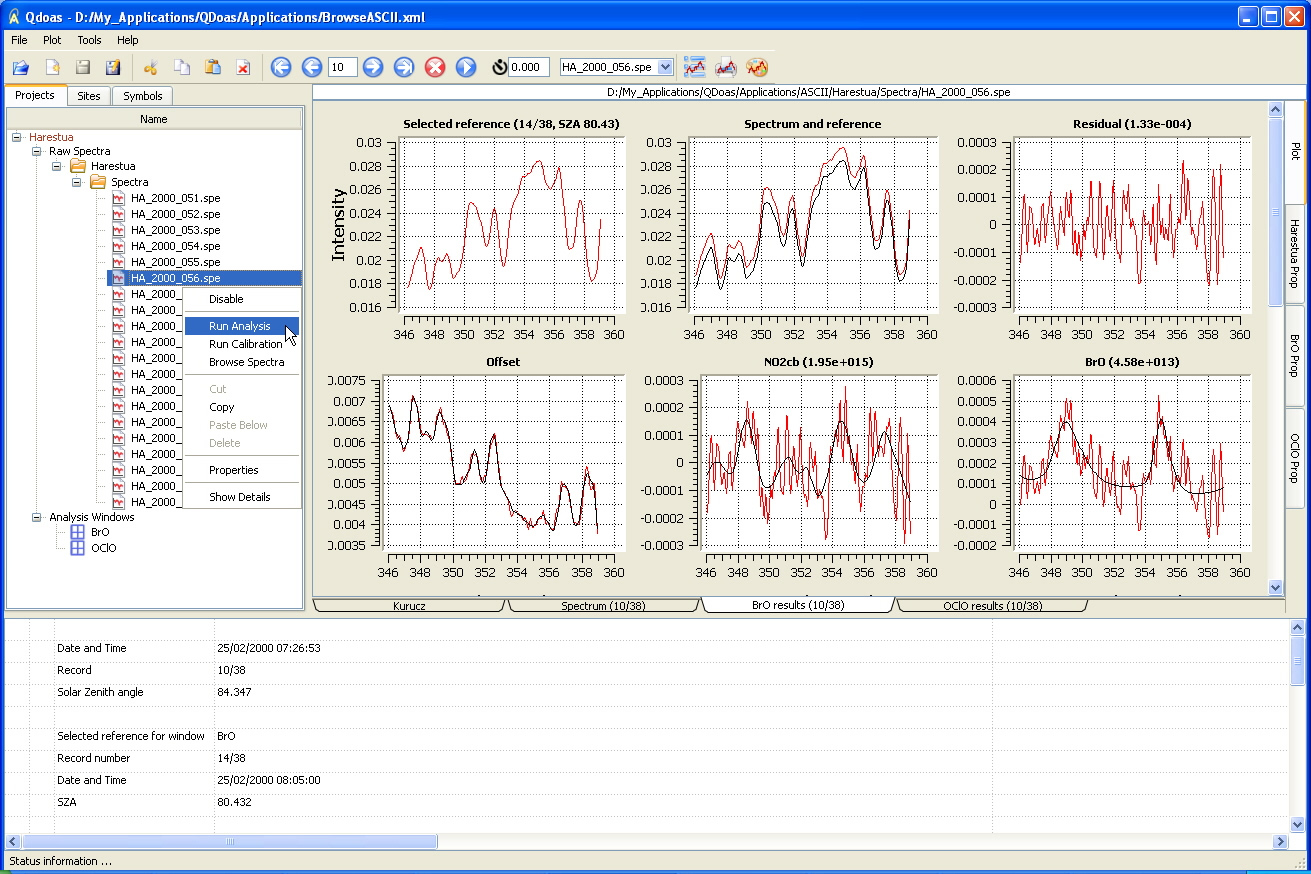
\includegraphics[width=1\textwidth,angle=0]{img/QDOAS_UI.jpg}
\end{center}

QDOAS user interface and configuration property sheets are distributed into three resizable panels with a fixed
arrangement~:

\begin{qdoasitem}
\item the elements of the application organized in tree structures
  presented in three tab pages (\textbf{Projects}, \textbf{Sites} and \textbf{Symbols}) in the
  upper-left one;
\item dialog boxes for the configuration of the elements of the
  application and the plot of spectra and results in the upper-right
  one; all the spectral windows are processed in one shot; right and
  bottom tab- switched access possible between all these pages;
\item the available information on the current spectrum and analysis
  results are displayed in the third one;
\end{qdoasitem}

\subsection{The Menu Bar}\hfill
\begin{minipage}[t]{\textwidth}
\vspace{-0.6\baselineskip}
\begin{tabular}[h]{p{2cm} p{9.5cm}}
\textbf{File} & Usual option to create a new application, open an existing
  one or save the current settings. QDOAS configuration files are in
  XML format.  \\ [6pt]
\textbf{Plot} & New option to organize the plots on the page (see below),
  to print the plot page or to save it in a png file; \\ [6pt]
\textbf{Tools} & The Convolution, Ring and undersampling tools are modules completely independent from the
  QDOAS application but they can still be called from the user
  interface;  \\ [6pt]
\textbf{Help} & Access to on-line help
\end{tabular}
\end{minipage}

\subsection{The Toolbar} \label{sec:interface_toolbar}
\hfill\vspace{-.8\baselineskip}

\includegraphics[width=\textwidth]{img/QDOAS_Toolbar.jpg}
The toolbar gives access to the same \textbf{File} and \textbf{Plot}
options of the menu bar. It contains also buttons to move easily in
the current file or to use another file in the case a multiple files
selection has been performed (very useful to browse spectra in the \textbf{MFC format (binary or std) generated by DOASIS} (cfr page \pageref{sec:MFC_DOASIS})).

\begin{minipage}{\textwidth} %minipage to force title and image to be on the same page
\subsection{Plot Properties}
\hfill\vspace{-.8\baselineskip}
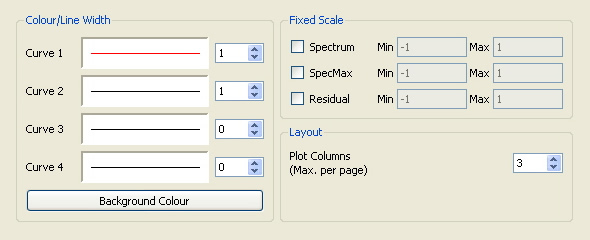
\includegraphics[width=\textwidth]{img/Plot_Properties.jpg}
This dialog box allows selecting a different color and a different
line thickness for curves 1 and 2 (respectively the spectrum and the
reference or the observed optical depth and the calculated optical
depth). The number of plot columns impacts the size of the plots.
\end{minipage}

\subsection{Handling plots}
It is not possible to display a specific plot in another window but zoom can be made by right-clicking the
\textbf{Interactive} option from \underline{\textbf{the title of a plot}}.

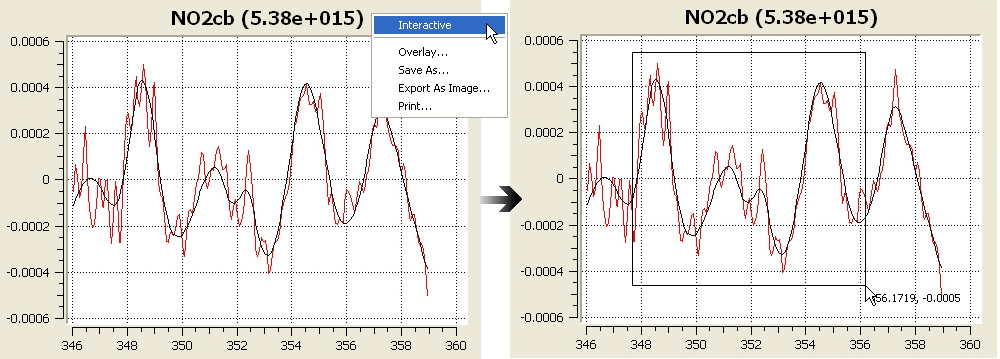
\includegraphics[width=\textwidth]{img/Plot_Zoom.jpg}

The \textbf{Save As} option saves the plotted curves in a ASCII file
(useful for example to create a reference spectrum). \textbf{Export As}
image exports the selected plot in a png file while \textbf{Print}
sends it to printer. \textbf{Overlay} will load a spectrum from a given file
and superpose it over the already plotted curves but this option is
not yet implemented.

\section{The projects tree}
The organisation of projects, analysis windows, spectra files and
directories in a tree structure completed with the definition of
right-click shortcut menus at each level of the tree makes the access,
manipulation and con\-fi\-gu\-ra\-tion of all these objects very easy.

\subsection{Raw Spectra}
Spectra to analyze have to be inserted under this projects tree
node. Individual files and complete directories structures are
accepted. The ``New Folder" option allows organizing spectra files and
directories within a user-defined catalog (folder that is not
physically present on the disk). The following actions can be
performed from any node:

\begin{tabular}[h]{p{3.5cm} p{8cm}}
\textbf{Browse Spectra} & browses spectra in the selected file(s); \\ [6pt]
\textbf{Run Analysis} & analyses spectra using the configuration
  of the project and analysis windows; this step includes the
  correction of the wavelength calibration of the reference spectrum
  if it has been requested in the configuration of the analysis
  windows; \\ [6pt]
\textbf{Run Calibration} & uses the options defined in the
  \textbf{Calibration page} of \textbf{Projects properties} (see page \pageref{sec:projects_calibration_page}) to apply it on
  spectra. \\ [6pt]
\textbf{Export Data/Spectra} & browses spectra and saves the selected fields in ASCII .  If only data on records are exported, the format is the same as QDOAS \textbf{output} files (see Annex, page \pageref{cha:output}); otherwise, spectra are saved in \textbf{Column extended format} (see Annex, page \pageref{cha:input-files-format}) \\ [6pt]
\end{tabular}

To move from one record to the other or from one file to the other (in
case of multiple files selection), use the adequate buttons in the
toolbar:

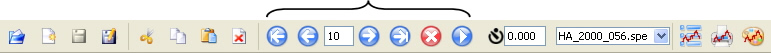
\includegraphics[width=\textwidth]{img/QDOAS_Toolbar2.jpg}

Other options~:

\begin{tabular}[h]{p{4cm} p{7.5cm}}
\textbf{Disable/Enable} & Disables the selected file or directory
  from the list of files to browse/analyze. Enable option re-enables
  previously disabled files. \\ [6pt]
\textbf{Refresh} & Refreshes the list of files in the selected
  directory;    \\ [6pt]
\textbf{Show/Hide Details} & Shows/hides file information (last
  modification date and time, size). The file size information is
  useful to indicate if the selected file is empty or not. \\ [6pt]
\end{tabular}


\subsection{Analysis windows}
A project can include several spectral analysis windows. A specific
analysis window can be disabled in order not to process it without
removing it from the list. The \textbf{View Cross Sections} option is
useful to check that the requested cross sections files exist.

\section{The observation sites}
In the \textbf{Observation Sites} page, a list of observation sites
can be specified by their location coordinates:

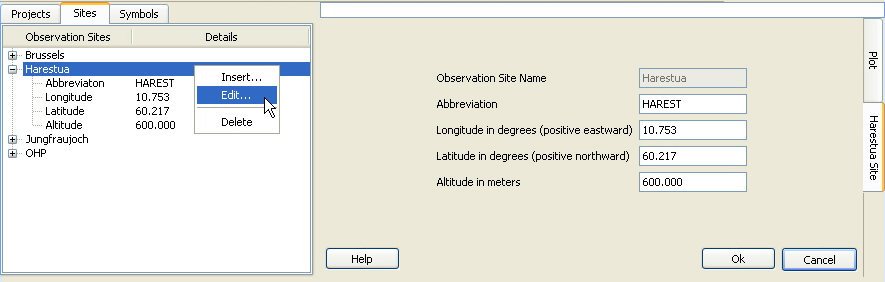
\includegraphics[width=\textwidth]{img/Observation_Sites.jpg}

QDOAS applies the following conventions~:

\begin{minipage}[t]{\textwidth}
\vspace{-1\baselineskip}
\begin{itemize} \itemsep -6pt
\item longitudes are positive eastwards; negative westwards;
\item latitudes are positive northwards; negative southwards.
\end{itemize}
\end{minipage}

For ground-based measurements, information on the observation site can
help to [re-]calculate the solar zenith angle as far as the
measurement date and time are correct (see the \textbf{Instrumental page}
 of \textbf{Projects properties}, page \pageref{sec:projects_instrumental_page}).
The longitude is also accounted to correctly select the reference spectrum of the day using the local time instead of the UT time in the case fractional days and times given in UT are distributed on two days (for example, for China data, two reference spectra could be selected for data of a same day before and after 00:00 UT if the observation site is not specified).

 For satellite
measurements, this page can be used to define a list of overpasses
(see the \textbf{Selection} page of Projects properties, page \pageref{sec:projects_selection_page}). In
both cases, the \textbf{Abbreviation} is used as prefix of the name of
the output files when the automatic creation of the output file name
is requested.

The \textbf{Altitude} information is just for the user.

\section{The symbols}
Before configuring the analysis, the user must define the list of all
relevant symbols that will be used. These symbols are needed to build
cross sections files filters, to link \gls{amf} and cross section files and
for internal manipulations (\textbf{Molecules} and \textbf{Shift and
  Stretch} pages of \textbf{Analysis Windows properties}).

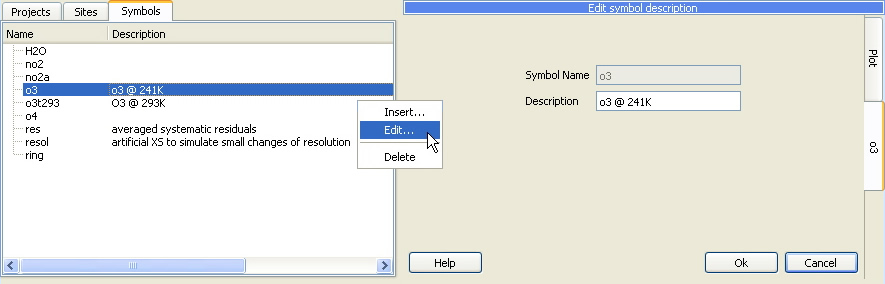
\includegraphics[width=\textwidth]{img/Symbols.jpg}

Cross sections symbols can be completed with a short description. The
deletion of a symbol is possible only if this symbol is not used in
the configuration of a project or an analysis window.

%%% Local Variables:
%%% mode: latex
%%% TeX-master: "QDOAS_manual"
%%% TeX-PDF-mode: t
%%% End:

\chapter{Description of Algorithms}\label{cha:descr-algor}
This chapter summarizes the main features of QDOAS and describes the
structure of the program and the algorithms.

\section{Differential Optical Absorption Spectroscopy}\label{sec:diff-optic-absorpt}
\gls{doas} is a widely used inversion method for the retrieval of
atmospheric trace gas abundances from multi-wavelength light
measurements.  It uses the structured absorption of many trace gases
in the UV, visible and near-infrared spectral ranges. The DOAS method
was originally developed for ground-based measurements
(\citet{platt1994,platt_2008}) and has been successfully adapted to
nadir measurements from UV-Vis space-borne spectrometers
(\citet{sciamachy}). It relies on the application of the Beer-Lambert
law to the whole atmosphere in a limited range of wavelengths.

The Beer-Lambert law states that the radiant intensity traversing a
homogeneous medium decreases exponentially with the product of the
extinction coefficient and the path length.  Applying this law to the
atmosphere, we obtain
\begin{equation}\label{eq:beer-lambert}
  I(\lambda)= I_0(\lambda)\exp \left( -\sum_{j=1}^{n} S^j(\lambda) c_j\right),
\end{equation}
where
\begin{itemize}
\item[$I_0$] is the spectrum at the top of the atmosphere, without extinction;
\item[$I$] is the measured spectrum after extinction in the atmosphere;
\item[$S^j$] is the absorption cross section of the species $j$, with
  wavelength dependent structures [cm2/molec.];
\item[$c_j$] is the column density of the species $j$ [molec./cm2].
\end{itemize}
The logarithm of the ratio of the spectrum $I_0$ (also called the
control spectrum) and the measured spectrum $I$ is denoted optical
density (or optical thickness) $\tau$
\begin{equation}\label{eq:optical_density}
\tau  \equiv \ln\left( \frac{I_0(\lambda)}{I(\lambda)}\right)= \sum_{j=1}^n S^j(\lambda) c_j .
\end{equation}
% explain here: reference spectrum/differential (s)cd's/doas approximations

The key idea of the DOAS method is to separate broad and narrow band
spectral structures of the absorption spectra in order to isolate the
narrow trace gas absorption features. In order to do this, some
approximations are made:
\begin{enumerate}
\item In the case where the photon path is not defined (scattered light
  measurements), the mean path followed by the photons through the
 atmosphere up to the instrument is considered;
\item The absorption cross sections are supposed to be independent of
  temperature and pressure, which allows us to introduce the concept
  of \glspl{scd};
\item Broadband variations, such as loss and gain from scattering and
  reflections by clouds and/or at the earth surface, are approximated
  by a common low order polynomial.
\end{enumerate}
Molecular absorption cross sections are fitted to the logarithm of the
ratio of the measured spectrum and the reference spectrum (i.e.\ an
extraterrestrial irradiance spectrum for satellite measurements, or a
spectrum measured around the local noon when the light path is minimum
for ground-based measurements). The resulting fit coefficients are the
integrated number of molecules per unit area along the atmospheric
light path for each trace gas, the differential \gls{scd}. The slant column depends
on the observation geometry, the position of the sun and also on
parameters such as the presence of clouds, aerosol load and surface
reflectance.

\section{DOAS retrieval}\label{sec:doas-retrieval}
\subsection{DOAS fitting}\label{sec:doas-fitting}
In the DOAS analysis, high frequency spectral structures of the
various absorbing species are used to resolve the corresponding
contributions to the measured optical density. This is achieved using
a least squares fitting procedure for the differential slant column
densities of the various species.  Large band contributions to the
atmospheric attenuation (Rayleigh and Mie scattering) are accounted
for by including a low order polynomial $P(\lambda) = \sum b_k
\lambda^k$ in the fit. Other effects, such as the Ring effect or
instrument undersampling can be treated as pseudo-absorbers.

According to eq.\ \eqref{eq:optical_density}, the DOAS retrieval is a
linear problem. This linearity is unfortunately broken down by the
need to account for additional effects, namely:
\begin{enumerate}
\item small wavelength shifts $\Delta(\lambda)$ between $I$ and $I_0$
  spectra must be corrected using appropriate shift and stretch
  parameters;
\item possible instrumental and/or atmospheric stray light or residual
  dark current signal require the introduction of an offset parameter.
\end{enumerate}
Including these necessary non-linear corrections and the polynomial
component $P(\lambda)$, we obtain the modified equation
\begin{equation}\label{eq:doas_non_linear}
\ln\left(
  \frac{I(\lambda-\Delta(\lambda))-\mathrm{offset}(\lambda)}{I_0(\lambda)}
  \right)+\sum_{j=1}^nS^j(\lambda)c_j +P(\lambda) = 0\,.
\end{equation}

\subsection{Marquardt-Levenberg Algorithm}\label{sec:marq-levenb-algor}
The \glspl{scd} $c_j$ can be retrieved by performing a least squares
fit of the measurement data to equation (\ref{eq:doas_non_linear}).
Due to the shift, stretch and offset parameters, this is a non-linear
least squares problem, which can typically be solved using a \gls{ml}
algorithm (see~\citet{Marquardt1963,Bevington1969}).  Starting from
given initial values, this algorithm searches the parameter space
using a combination of Gauss-Newton and gradient descent steps.  The
\gls{ml} algorithm is an efficient minimization algorithm for a wide
range of non-linear functions, but it may converge to a local minimum
if the initial values are too far from the global minimum.  In QDOAS,
this problem can occur during the wavelength calibration, when the
initial calibration is not accurate enough (see
\nameref{sec:calibration-problems} in section
\ref{sec:analysis-problems} of the appendix).

% explain offset modelling?
In QDOAS, the M-L algorithm is used to find the set of parameters that
minimizes the weighted\footnote{Weighting the residuals by the
  instrumental errors $\sigma^i$ is optional in QDOAS.  When no
  measurement uncertainties are used (or no error estimates are
  available), all uncertainties in equation~\eqref{eq:sum_of_squares}
  are set to $\sigma^i=1$, giving all measurement points equal weight
  in the fit.  See analysis properties in section
  \ref{sec:projects_analysis_page}} sum of squares
%\begin{equation}\label{eq:sum_of_squares}
%  S = \sum_{i=1}^M \left(\frac{Y^i - Y_{\mathrm{fit}}^i}{\sigma^i}\right)^2,
%\end{equation}
\begin{align}
  F(\vec{\alpha}) = & \frac{1}{2} \sum_{i=1}^M\left(
    \frac{f^i(\vec{\alpha})}{\sigma^i}
    \right)^2 \nonumber \\
    = &\frac{1}{2} \sum_{i=1}^M
  \left(
    \frac{\ln(I^i(\vec{a}))+\sum_{j=1}^{n}S^{ij} c_j + \sum_{k=0}^d
      b_k (\lambda_i)^k -\ln(I^i_0)}{\sigma^i}
  \right)^2,  \label{eq:sum_of_squares}
\end{align}
where
\begin{description}
\item[$\vec{\alpha}=(\vec{a},\vec{b},\vec{c})$] is the vector
  containing all fitted parameters;
\item[$\vec{a}$] is the set of parameters describing the shift,
  stretch and offset of the measured spectrum;
\item[$b_k,\, k=1,\ldots,d$] are the fitted polynomial coefficients;
\item[$c_j,\, j=1,\ldots,n$] are the fitted \glspl{scd};
\item[$\lambda_i,\, i=1,\ldots,M$] is the wavelength grid of the
  reference spectrum $I_0$, calibrated with respect to a high
  resolution solar spectrum (see section \ref{sec:wavel-calibr}).
\item[$I^i(\vec{a})$] is the measured spectrum, including shift,
  stretch and offset corrections, interpolated at wavelength
  $\lambda_i$;
\item[$S^{ij}$] is the absorption cross section of absorber species
  $j$, as measured in a laboratory, interpolated at wavelength
  $\lambda_i$;
\item[$I^i_0$] is the reference spectrum at wavelength $\lambda_i$ and
\item[$\sigma^i$] is the standard error on the measurement at
  wavelength $\lambda_i$.
\end{description}
In each iteration, the fitting algorithm will choose new values for
the parameters using the Marquardt-Levenberg algorithm, and recompute
the sum of squares $F$.  The algorithm assumes that it has converged
to a solution when the difference between two succeeding values of $F$
is smaller than a fixed small number $\epsilon$.  The convergence
criterion $\epsilon$ can be chosen by the user (see
\nameref{sec:conv-crit} in section \ref{sec:projects-properties}).

For a given value of the non-linear parameters $\vec{a}$, the
determination of the parameters $c_j$ and the polynomial coefficients
$b_k$ is a linear least squares problem.  Explicitly, we can rewrite
equation~\eqref{eq:sum_of_squares} as
\begin{equation}
  \label{eq:doas_linear}
  F = \frac{1}{2}\sum_{i=1}^M\left(
    \frac{\ln(I^i(\vec{a})/I^i_0) +  (A \cdot \vec{x})^i}{\sigma^i}
    \right)^2\,,
\end{equation}
where the matrix $A$ contains the polynomial basis $(\lambda_i)^k,
k=0,\ldots,d$ and the absorption cross sections $S^{ij}, j=1,\ldots,n$
and $\vec{x}$ represents the combined linear parameters $\vec{b}$ and
$\vec{c}$:
\begin{align}
  \label{eq:doas_linear_matrix}
  A^{il}  & = \left( (\lambda_i)^d \quad S^{ij} \right)\,,\\
  \vec{x} & = \left( \begin{array}{c}
      \vec{b}\\
      \vec{c}
    \end{array}\right)\,.
\end{align}
% describe linear equation here?
This fact is exploited in QDOAS to limit the parameter space of the
\gls{ml} algorithm to the non-linear parameters: once a new set of
values $\vec{a}'$ for the non-linear parameters is chosen, the linear
parameters $b_k$ and $c_j$ are updated using a linear least squares
algorithm, minimizing the sum of squares \eqref{eq:sum_of_squares} for
the given values of the non-linear parameters.

In QDOAS, the linear least squares problem is solved using the QR
decomposition of the matrix $A$ defined in equation
\eqref{eq:doas_linear_matrix}.

QDOAS can include further parameters in the fits
(\ref{eq:sum_of_squares}), which we omitted from the previous
description for the purpose of clarity.  Such parameters include the
width of the instrument's slit function and wavelength shifts in the
reference absorption cross sections $S^j(\lambda)$.  Mathematically,
they play the same role as the shift, stretch and offset parameters
$\vec{a}$.  Section \ref{sec:analysis_config_param} describes the
available fitting options in QDOAS and their
\index{configuration}configuration.

\subsection{Intensity fitting}\label{sec:intensity-fitting}
QDOAS also supports the so-called intensity fitting (or direct
fitting) method where measured intensities are directly fitted instead
of their logarithms. The equation used in the least squares fitting
procedure is then
\begin{equation}
  \label{eq:intensity_fitting}
  \frac{I(\lambda -\Delta(\lambda)) - \mathrm{offset}(\lambda)}{ I_0(\lambda)} - P \exp(-\sum_{j=1}^n S^jc_j) = 0\,,
\end{equation}
This method involves a decomposition of equation
(\ref{eq:intensity_fitting}) in its linear and non-linear parts:
column densities are fitted non-linearly, but the polynomial, which is
taken out of the exponential function using a Taylor expansion, and
offset are linear parameters.

Intensity fitting is sometimes preferred to optical density fitting,
for example when a poor signal leads to numerical problems when taking
the logarithms of the intensity ratio.

\subsection{Errors On Slant Column Densities}\label{sec:errors-slant-column}
% TODO: remark that errors sigma are errors on log(I) in case of
% optical density fitting, and errors on I in case of intensity
% fitting?
Uncertainties on the retrieved slant columns $c_j$ depend on:
 \begin{itemize}
 \item the sensitivity of the sum of squares $F$
   (\ref{eq:sum_of_squares}) with respect to variations of the fitted
   parameters around the minimum and
 \item the noise on the measurements.
 \end{itemize}

 Formally, the covariance matrix of the fitted parameters of a least
 squares estimate may be estimated by the inverse of the Hessian of
 the sum of squares $F$, evaluated at the fitted values of the
 parameters
\begin{equation}
  \label{eq:slnterr_general}
  \Sigma_{\vec{\alpha}} = H^{-1}\,,
\end{equation}
where $H$ is given by
\begin{equation}
  \label{eq:hessian}
  H_{kl} = \frac{\partial^2 F}{\partial \alpha_k \partial \alpha_l}\,.
\end{equation}

The actual approach used to calculate $H$ in QDOAS is different in
optical density fitting mode and in intensity fitting mode.  In
optical density fitting mode, the slant column density is fitted
linearly according to equation~\eqref{eq:doas_linear} and we use the
following expression for the covariance matrix $\Sigma_{\vec{x}}$ of
the weighted linear least squares parameter estimate:
\begin{equation}
  \label{eq:slnterr_linear}
  \Sigma_{\vec{x}} = \left(A^T W^2 A\right)^{-1}\,,
\end{equation}
where the matrix $A$ contains the linear components of the fit, as
described in equation~\eqref{eq:doas_linear_matrix} and the $(M \times
M)$ diagonal matrix $W$ contains the measurement errors
\begin{equation}
  \label{eq:weight_matrix}
  W_{ij} = \frac{1}{\sigma^i}\quad \mathrm{if}\, i=j\,.
\end{equation}
Equation \eqref{eq:slnterr_linear} implies that uncertainties on
estimated values of the non-linear parameters are not taken into
account in the reported errors on the slant columns.

When the individual measurement errors $\sigma^i$ are not available
(or the user has chosen not to weight the fit by the instrumental
errors), the weight matrix $W$ is just the identity matrix.  In this
case, the mean squared error on the measurements $\sigma^2$ may be
estimated by the reduced $\chi^2$, e.g.\ the sum of squares of the
residuals divided by the number of degrees of freedom in the fit
\begin{equation}
  \label{eq:chi_square}
  \chi^2 = \frac{\sum_{i=1}^M (f^i)^2 }{M-N}\,,
\end{equation}
where $M$ is the number of wavelengths included in the fit, and $N$ is
the total number of fitted parameters.
Equation~\eqref{eq:slnterr_linear} then becomes
\begin{equation}
  \label{eq:slnterr_linear_noweighting}
  \Sigma_{\vec{x}} = \chi^2\left(A^T A\right)^{-1}\,.
\end{equation}

In intensity fitting mode, the slant column densities are determined
using non-linear least squares fitting, and the Hessian is
approximated by the square of the Jacobian of the fitting functions
$f^i$
\begin{equation}
  \label{eq:hessian_approx}
  H_{kl} \simeq \sum_{j=1}^M \frac{\partial f^j}{\partial \alpha_k}\frac{\partial f^j}{\partial \alpha_l}\frac{1}{(\sigma^j)^2}\,.
\end{equation}
This implies that, in intensity fitting mode, uncertainties on the
linear parameters are not taken in to account in the reported slant
column errors.  As in the linear case, when the instrumental errors
are not used or not available, the $\sigma^j$ in equation
\eqref{eq:hessian_approx} are replaced by 1, and the measurement error
is approximated using the reduced $\chi^2$ of the fit instead.
Equation~\eqref{eq:slnterr_general} then becomes
\begin{equation}
  \label{eq:slnterr_nonlinear_noweighting}
  \Sigma_{\vec{\alpha}} = \chi^2 H^{-1}\,.
\end{equation}
% in practice, there are even some L-M modifications to this formula.

\subsubsection{Limitations}
The estimates for the uncertainties of the fitted parameters rely on
the statistical model used for the DOAS retrieval.  The model assumes
that the errors on the measurements at each frequency are independent
and normally distributed.  When measurement errors are correlated
or contain systematic components, or in case of fitting errors such
as a wrong fit for shift and stretch parameters, or relevant
absorbers that are not included in the fit, the uncertainties
calculated by QDOAS will underestimate the true error on the slant
column density.  Remaining residual structures after the fit, or a
value of $\chi^2 \gg 1$ when measurement errors $\sigma^i$ are taken
into account, are an indication of such a bad fit.  A discussion can
be found in~\citet{stutz_1996}.

We also note that the errors in QDOAS do not take into account the
uncertainties on the cross sections. A way to achieve this is given
in~\citet{Theys2007}.

\section{Wavelength calibration}\label{sec:wavel-calibr}
The quality of the retrieval fit strongly depends on a perfect
alignment between the spectrum to analyze, the reference spectrum and
the cross sections. The wavelength-pixels relation
(see~\citet{platt_2008}) of the % or just give expression here?
reference spectrum, previously determined in laboratory using a lamp
spectrum % what's the laboratory lamp spectrum doing here?
can be corrected using a procedure based on the alignment of the
Fraunhofer structures of the reference spectrum $I_0$ with those of an
accurately calibrated high-resolution solar reference atlas, degraded
at the resolution of the instrument, i.e. convolved with the
instrumental slit function. The reference atlas used for this purpose
is usually the~\citet{Chance2010} spectrum.

During the calibration process, the instrumental slit function can
also be characterized by repeatedly convolving the highly resolved
solar atlas with the slit function and adjusting the parameters until
the best match with the reference spectrum is found.  QDOAS allows
fitting the parameters of different line shapes, as well as their
wavelength dependence.  This is useful when the slit function provided
with the instrument is not described precisely enough in the
wavelength interval used for the retrieval.  In the same way, to
account for the moderate resolution of satellite or ground-based
instruments (about a few tenths of a nanometer), the absorption cross
sections of the trace gases have to be convolved with the instrumental
slit function (and interpolated on the final $I_0$ wavelength grid). A
good knowledge of the instrumental slit function and its potential
wavelength variation is important to avoid systematic errors in the
retrieved slant columns due to spectral shape mismatch between the
reference and atmospheric spectra~\citep{vanroozendael2002}.

\subsection{Fit of shift and stretch}\label{sec:fit-shift-stretch}
Shift and stretch (see \nameref{sec:shift} on page
\pageref{sec:shift}) can be taken into account in the wavelength
calibration scheme. To this end, the spectral interval is divided into
a number of sub-intervals.  By default, QDOAS will split the complete
calibration interval into equally sized disjoint sub-intervals, but
more advanced options are available, too (see
\nameref{sec:calibration-windows} on page
\pageref{sec:calibration-windows}).  The fitting algorithm used for
the DOAS retrieval is then applied in each sub-interval to fit the
measured intensities to those of the high-resolution solar spectrum,
according to the equation
\begin{equation}
  \label{eq:calibration_shift}
  I_0(\lambda)= I_S(\lambda - \Delta_i - a_i(\lambda-\lambda_{\mathrm{c},i}))\exp(-\sum_{j=1}^mS^jc_j)\,,
\end{equation}
where $I_S$ is the solar spectrum convolved at the resolution of the
instrument, $\Delta_i$ is a fitted constant shift in sub-interval $i$,
$\lambda_{\mathrm{c},i}$ the central wavelength of sub-interval $i$,
$a_i$ the interval's fitted stretch factor, and the $c_j$ are optional
absorber coefficients accounting for possible light absorption in the
reference spectrum $I_0$.  Typically, the calibration uses more then
one sub-interval, and we fit a polynomial through the pairs
$(\lambda_{\mathrm{c},i}, \Delta_i)$ in order to reconstruct an
accurate wavelength calibration $\Delta(\lambda)$ for the complete
analysis interval.  When the calibration is set to use only a single
interval, the shift and stretch values from this interval are used to
calculate the optimized wavelength grid for the analysis.

Several tests may be needed to determine the best configuration. One
has to find the right compromise between using enough sub-intervals to
represent the wavelength variation of the shift, and having enough
spectral information in each sub-window.  The interval calibration
should cover all analysis spectral windows.

The algorithm can take into account molecular absorption and offset
correction.  In order to help the algorithm to converge to the correct
solution, it is important to start with a preliminary wavelength grid
close enough to the real one and to limit the number of fitting
parameters (for example by fixing the value of some parameters,
typically the concentration of the fitted molecules after a first
estimation).  Another option to help the algorithm converge is to
determine the initial shift by testing for correlation:

\subsection{Calculation of the preshift}
When the wavelength shift between the high-resolution solar atlas and
the initial calibration of the reference spectrum is too large, the
fitting algorithm used in the calibration procedure may not converge
to the proper value.  If you find that this is the case, you can
choose to perform an extra ``preshift'' calculation.  With this
option, QDOAS performs the following extra steps before running the
wavelength calibration algorithm:

\begin{enumerate}
\item The high-resolution solar spectrum is degraded to instrument
  resolution using the chosen slit function settings.  If slit
  function parameters are also fit during the calibration, their
  initial values are used for this step.
\item The convolved solar spectrum and the reference spectrum are
  smoothed and normalized, with an averaging bandwidth of about 5nm.
\item Using the Nelder-Mead optimization algorithm, QDOAS determines
  the shift value resulting in the highest correlation between the
  reference and high-resolution solar spectrum.
\end{enumerate}

After this preshift step, QDOAS performs the regular wavelength
calibration on the original spectra, using the preshift value as the
initial value for the calibration shift in each sub-interval.

\subsection{Ref2/Ref1 Alignment}\label{sec:ref2ref1-alignment}
If two reference spectra are given (see section
\ref{sec:projects-properties} and figure
\ref{projects_properties_calibration}), the wavelength calibration
described in the previous section is applied to the first one.  The
shift between both reference spectra is then determined using a least
squares fit.  This shift is then applied to the reference absorption
cross sections in order to align them on the second reference
spectrum.  The measured spectra are then analyzed with respect to the
second reference spectrum.

% in detail:
% pixels are chosen based on pixel/wavelength relationship from corrected reference 1 grid,
% same pixels are selected from reference 2
% shift between ref1/ref2 is fitted
% this shift is applied to the cross sections
%
% motivation for all this?
% possibility to take solar spectrum by instrument & earthshine
% spectrum, and calibrate in two steps?
% why don't we correct the wavelength grid of reference 2?

\subsection{Characterization Of The Line
  Shape}\label{sec:char-line-shape}
If the slit function varies strongly in the fitting window and is
symmetric enough to be approached by an analytical function like a
Gaussian, it can be fitted together with the shift during the
calibration procedure.  A high resolution solar spectrum is needed.
The wavelength variation of the line shape can be accounted for in
order to convolve high-resolution cross sections before the
analysis. % should describe this more clearly... we mean varying width
          % across spectral interval?
The equation \eqref{eq:calibration_shift} used in the calibration is
then modified as follows:
\begin{equation}
  \label{eq:calibration_shift_lineshape}
  I_0(\lambda) = (L_{a_i}\ast I_S)(\lambda-\Delta_i)
  \exp\left(-\sum_{j=1}^m c_j S^j\right)\,,
\end{equation}
where $L_{a_i}(\lambda)$ is the line shape with \gls{fwhm}
parametrized by $a_i$.  QDOAS can fit the parameters for a number of
different analytical line shapes, which we describe in more detail in
the \nameref{sec:analyt-line-shap} section on page
\pageref{sec:analyt-line-shap}.

\section{Fit parameters}\label{sec:fit-parameters}
\subsection{Absorption cross sections}\label{sec:absorpt-cross-sect}
In principle, DOAS measurements are applicable to all gases with
suitable narrow absorption bands in the UV, visible or near IR
regions. However, the generally low concentrations of these compounds
in the atmosphere and the limited signal-to-noise ratio of the
spectrometers restrict the number of trace gases that can be detected.
Figure \ref{fig:doas_cross_sections} shows the absorption cross
sections of a number of trace gases that are regularly measured using
the DOAS technique.

\begin{figure}
  \centering
  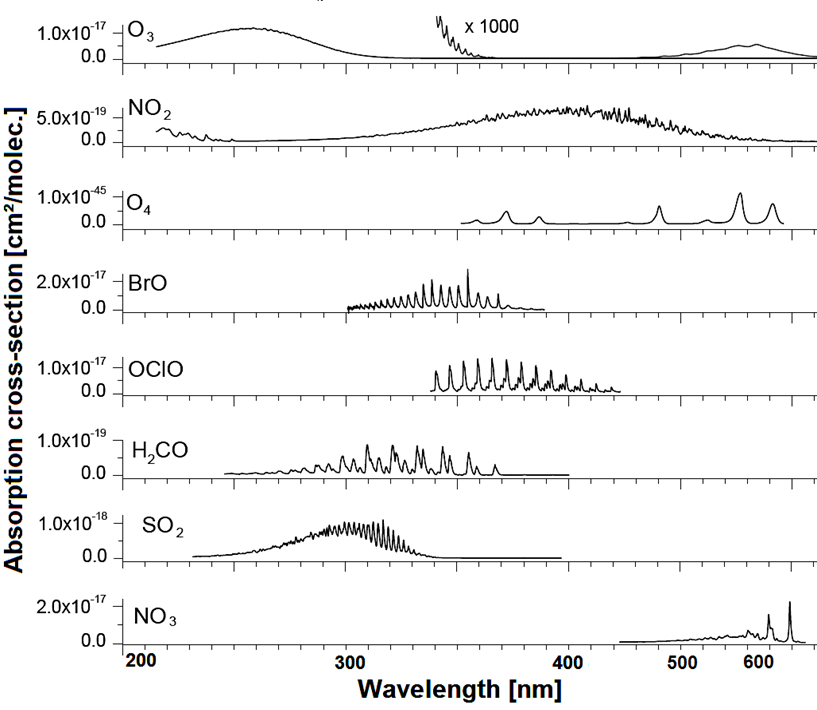
\includegraphics[width=0.9\textwidth]{Algo_Cross.jpg}
  \caption{Absorption cross sections of various absorbers retrieved with
the DOAS method (figure taken from~\citet{platt_2008}).}
\label{fig:doas_cross_sections}
\end{figure}

Many spectral regions contain a large number of interfering
absorbers. In principle, because of their unique spectral structure, a
separation of the absorption is possible.  However, correlations
between absorber cross sections sometimes lead to systematic biases in
the retrieved slant columns.  In general, the correlation between
cross sections decreases if the wavelength interval is extended, but
doing so is at odds with the assumption that a single effective light
path for the entire wavelength interval is defined, leading to
systematic misfit effects that may also introduce biases in the
retrieved slant columns.  To optimize DOAS retrieval settings, a
trade-off has to be found between these effects.  A basic limitation
of the classical DOAS technique is the assumption that the atmosphere
is optically thin in the wavelength region of interest.  At shorter
wavelengths, the usable spectral range of DOAS is limited by rapidly
increasing Rayleigh scattering and \ozone{} absorption.  In addition,
‘line-absorbers’ such as \water, \oxygen, CO, \CO2 and \CH4 usually
cannot be retrieved precisely by standard DOAS algorithms because
their strong absorption also depends on pressure and temperature.

The selection of the spectral analysis window determines which
absorbers have to be included in the fitting procedure. The pressure
dependence of absorption cross sections can be neglected in UV-Visible
region. However, the temperature dependence of cross sections can be
significant (for example that of \ozone{} and \NO2). This can be
corrected in a first approximation by introducing correction factors
during the \gls{amf} calculation~\citep{Boersma2004} or,
assuming a linear dependence on temperature, by fitting two absorption
cross sections at different temperatures as described
in~\citet{vanroozendael2002}.

\subsubsection{Shift}\label{sec:shift}
Before analysis, absorption cross sections are interpolated on the
final grid of the reference spectrum which may be determined by the
program itself (automatic reference selection mode). Moreover, shift
and stretch parameters can be fitted during the processing of a
spectrum in order to obtain the best match of the absorption
structures.

\subsubsection{Interpolation/Convolution}
Cross sections can be pre-convolved and interpolated\footnote{By
  default, QDOAS uses cubic spline interpolation.} on an appropriate
wavelength grid prior to the analysis. However, the direct use of
high-resolution cross sections which can be convolved in real-time
with a predefined slit function or with the slit function determined
by the wavelength calibration procedure, is more convenient.

\subsubsection{Differential cross sections}
The aim of calculating differential absorption cross sections is to
separate narrow spectral features from unstructured absorption not
useful in the DOAS method.  Figure
\ref{fig:differential_cross_section} gives an illustration.

\begin{figure}
  \centering
  \begin{tabular}{cc}
    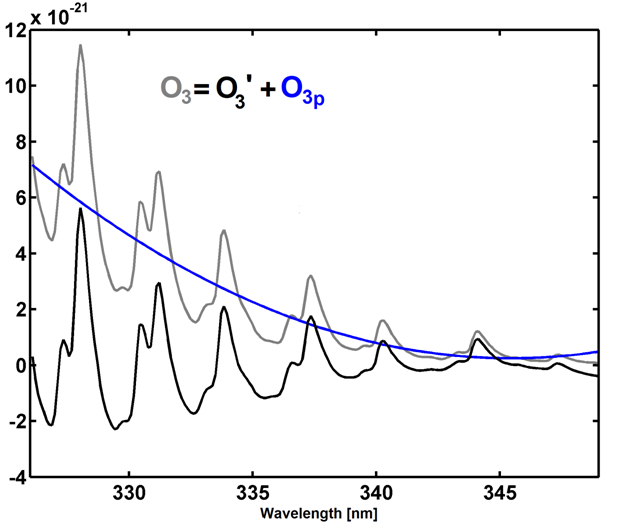
\includegraphics[width=0.45\textwidth]{Algo_Cross_1.jpg}
    & 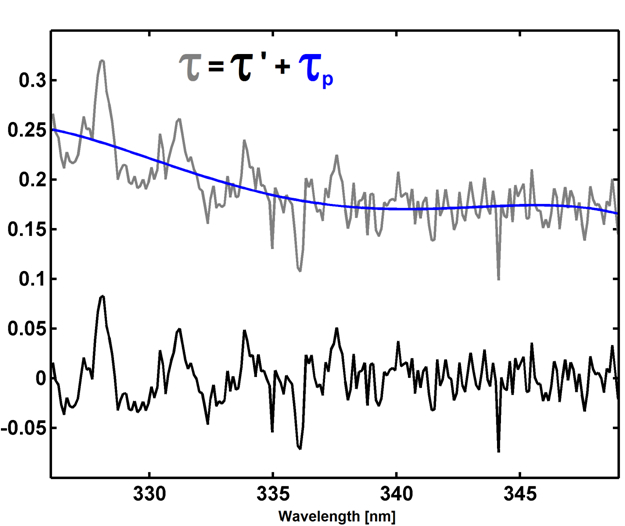
\includegraphics[width=0.45\textwidth]{Algo_Cross_2.jpg}
  \end{tabular}
  \caption{Cross section $\mathrm{O}_3$ and optical thickness $\tau$ are separated into a narrow ($\mathrm{O}_3'$ and $\tau'$)
and a broad band part ($\mathrm{O}_{3p}$ and $\tau_p$) by
an adequate filtering procedure.}
\label{fig:differential_cross_section}
\end{figure}

Differential cross sections can be calculated by orthonormalization
with respect to an orthogonal set formed with the low order component
vectors (usually a base of order 2 or 3) of the polynomial.  The
vectors are orthogonalized using the Gram-Schmidt
algorithm.  This method gives also the possibility to separate the
spectral structures of temperature dependent cross sections by
mutually orthogonalizing them.  Differential cross sections can
alternatively be obtained by high-pass filtering: a filter is applied
iteratively on the cross section and the resulting cross section is
subtracted from the original one. High-pass filtering is presently
only supported in optical density fitting mode (DOAS mode).  Note that
it is not necessary to calculate differential cross sections when the
baseline is around 0 such as for \water, \tetraox{} or \H2CO.

\subsubsection{Low-pass filtering}
Low-pass filters can be applied to both spectra and absorption cross
sections. A large choice of filters is proposed (see `Filtering
Page', section \ref{sec:projects_filtering_page}).

\subsubsection{Wavelength-dependent AMF}
Absorption cross sections can be replaced by geometrically corrected
cross sections that take into account the wavelength dependency of the
\gls{amf}. The correction is based on the equation
\begin{equation}
  \label{eq:wavelength_dep_amf}
  \ln(I_0)-\ln(I) = S(\lambda) \mathrm{AMF}(\lambda,\mathrm{SZA})\,,
\end{equation}
where $\mathrm{AMF}(\lambda,\mathrm{SZA})$ is the AMF calculated for a
given wavelength $\lambda$ and a given \gls{sza}.
% fitted density is then already the vertical column density?

\subsection{Polynomial}\label{sec:polynomial}
In the DOAS technique, absorption cross sections of the considered
mole\-cules are highly structured, while scattering by molecules and
particles (Rayleigh and Mie scattering), as well as reflection at the
surface, have broadband dependencies that can be approximated by a low
order polynomial. In QDOAS, polynomials up to degree 5 can be
fitted. The low order components of the polynomial can be used to
calculate differential cross sections when this is preferred to
high-pass filtering.

\subsection{Shift and Stretch}\label{sec:shift-stretch}
Shift and stretch parameters allow to correct possible misalignment
between the various wavelength-dependent quantities involved in the
data evaluation (i.e.\ measured and reference spectra as well as
absorption cross sections).  Shift and stretch parameters may be
fitted or simply applied to any wavelength-dependent quantity,
according to the equation
\begin{equation}
  \label{eq:shift_stretch}
  \Delta\lambda = a + b(\lambda-\lambda_0) + c(\lambda-\lambda_0)^2\, ,
\end{equation}
where $\lambda$ is the wavelength according to the original
calibration and $\lambda_0$ is the center wavelength of the current
spectral range.  The parameters $a$,$b$ and $c$ describe the offset
and the first and second order stretch applied to $\lambda$.

\subsection{Offset Correction}\label{sec:offset-correction}
An ideal spectrometer in an ideal atmosphere would measure the part of
the sunlight that has been elastically scattered by air molecules and
particles.  In a real experiment, however, a number of possible
additional sources may contribute to the measured intensity, adding an
“offset” to the ideal Rayleigh/Mie contribution.  In addition to the
Ring effect, which is, to a first approximation, a natural source of
offset, one must also account for instrumental sources of offset, such
as stray light in the spectrometer and dark current of the detector.
The offset component in equation~\eqref{eq:doas_non_linear} accounts
for these effects.  QDOAS models the offset using a polynomial
\begin{equation}
  \label{eq:offset}
  \mathrm{offset}(\lambda) = (a + b(\lambda-\lambda_0) + c(\lambda-\lambda_0)^2) \bar{I}\, ,
\end{equation}
where $\lambda_0$ is the center wavelength of the spectral analysis
window, $\bar{I}$ is the average intensity and $a$, $b$ and $c$ are
fitted parameters.

Due to the normalization by $\bar{I}$, the offset values can be easily
interpreted relatively to the absolute intensity of the spectrum
(percent offset).  In DOAS, the offset is usually fitted as a
non-linear parameter.  Sometimes, this could lead to numerical errors
in the evaluation of the logarithm, typically in the near UV region
where the level of the signal is very low.  In this case, we can fit
the offset as a linear parameter.  Expanding the left-hand side of
equation~\eqref{eq:doas_non_linear} to first order, we obtain
\begin{equation}
  \label{eq:offset_linear}
  \ln(I(\lambda -\Delta(\lambda))) = \ln(I_0(\lambda))-\tau(\lambda) + \frac{\mathrm{offset}(\lambda)}{I(\lambda+\Delta\lambda)}\,.
\end{equation}
 % why not also normalize with respect to average intensity in this case?

\subsection{Ring Effect}\label{sec:ring-effect}
Because of \gls{rrs}, a small fraction of the
incident photons undergo a wavelength change of a few nanometres,
i.e.\ a part of the scattering is inelastic. This causes an intensity
loss at their incident wavelength and a gain at the neighbouring
wavelengths to which they are redistributed.  RRS causes the so-called
“filling-in” of Fraunhofer lines, which have a slightly different
shape in the earthshine radiance than in the direct solar light.  This
effect was first discovered by~\citet{grainger_1962} and is referred
to as the Ring effect.  The atmospheric absorption lines are also
broadened by RRS events occurring after absorption (molecular Ring
effect).  Although RRS accounts for only a few percent of the measured
intensity, it significantly affects DOAS measurements of scattered
radiation since typical trace gas absorptions are of the order of a
percent or less.  If not properly corrected, the Ring effect produces
strongly structured residuals in the differential optical density, due
to the fact that Fraunhofer lines do not cancel perfectly between $I$
and $I_0$. Especially in the UV spectral range, the remaining spectral
structures can by far exceed the structures of weak atmospheric
absorbers.

Usually the Ring effect is taken into account by including an
additional ‘absorber’ in the DOAS fit. Ring cross sections
$S_{\mathrm{Ring}}(\lambda)$ can be
measured~\citep{Solomon_Schmeltekopf_Sanders_1987} or
calculated~\citep{Chance1997}. The Ring effect can be approximated
using the following development for an optically thin
atmosphere~\citep{Wagner1999,vanroozendael2002}:

One can consider that in any scattered light observation, the light
detected by the satellite instrument ($I_\mathrm{meas}$) is the sum of
elastic and inelastic scattering processes:
\begin{equation}
  \label{eq:rrs_i_meas}
  I_\mathrm{meas} = I_{\mathrm{elastic}} + I_{\mathrm{RRS}} = I_0 e^{-\tau} + I_{\mathrm{RRS}}\,.
\end{equation}
To analyze a measured spectrum, the logarithm of $I_{\mathrm{meas}}$
is taken. Since $I_{\mathrm{RRS}}$ is very small compared to
$I_{\mathrm{elastic}}$, the logarithm can be approximated by the first
two terms of the Taylor expansion:
\begin{equation}
  \label{eq:rrs_expand_i_meas}
  \ln(I_\mathrm{meas}) = \ln(I_{\mathrm{elastic}}) + \frac{I_{\mathrm{RRS}}}{I_{\mathrm{elastic}}}
  = \ln I_0 - \tau + \frac{I_{\mathrm{RRS}}}{I_{\mathrm{elastic}}} \,.
\end{equation}
The last term $I_{\mathrm{RRS}}/I_{\mathrm{elastic}}$ is the Ring term
which can be approximated by the product of a Ring coefficient
$\alpha_{\mathrm{Ring}}$ and a Ring cross section
$S_{\mathrm{Ring}}$. $\alpha_{\mathrm{Ring}}$ can be fitted together
with other absorbers in the DOAS procedure.

A good approximation of the Ring cross section can be obtained from
calculation of a source term $I_0^{\mathrm{Raman}}$ for Raman
scattering derived by simple convolution of the solar spectrum with
Raman cross sections, i.e with calculated \N2 and \oxygen{} RRS cross
sections. The term $I_{\mathrm{RRS}}/I_{\mathrm{elastic}}$ in
equation~\eqref{eq:rrs_expand_i_meas} is then substituted by
$\alpha_{\mathrm{Ring}} S_{\mathrm{Ring}}$ (where $S_{\mathrm{Ring}}
=I_0^{\mathrm{Raman}}/I_0$), assuming that the molecular Ring effect
can be neglected~\citep{Chance1997}. The QDOAS Ring tool calculates a
Ring cross section according to this
approach~\citep{Wagner1999}. The normalization of the Raman spectrum is optional.

\subsection{Undersampling Correction}\label{sec:unders-corr}
The undersampling is a well-known problem of
GOME~\citep{Chance1998}. It arises from the poor sampling ratio of the
GOME instrument, which results in a loss of spectral information when
interpolating earthshine spectra during the DOAS fitting
process. Undersampling is only a major problem when the sampling ratio
is close to 1.  In the case of GOME, this ratio is estimated at
0.16/0.112=1.43 at 340 nm.

The undersampling artifacts can be corrected using an ad-hoc cross
section obtained by simulating the effect based on a high-resolution
solar reference~\citep{Chance1998}.  This cross section is fitted as a
linear parameter, in both intensity fitting and in optical density
fitting modes.  The procedure to calculate the correction differs
slightly between the two fitting modes:

In intensity fitting mode, oversampled
and undersampled spectra are calculated as follows:
\begin{equation}
  \label{eq:undersampling}
  U(\lambda+\Delta) = \mathrm{over}(\lambda+\Delta) - \mathrm{under}^{(\Delta)}(\lambda)\,,
\end{equation}
where $\mathrm{over}(\lambda + \Delta)$ is a high-resolution solar
spectrum convolved on its original grid and interpolated on the final
grid $\lambda + \Delta$ and $\mathrm{under}^{(\Delta)}(\lambda)$ is a
high-resolution solar spectrum convolved on grid $\lambda$ and
subsequently interpolated on the final grid $\lambda + \Delta$.
% does it make a difference if we convolve on one grid or another?

Residuals are improved by adding a “second phase” of undersampling
\begin{equation}
  \label{eq:undersampling2}
  U_2(\lambda) = \mathrm{over}(\lambda) - \mathrm{under}^{(\Delta)}(\lambda)\,.
\end{equation}
In optical density fitting, we fit the logarithm of the ratio of the
measured intensities.  We therefore use the corresponding equations
\begin{align}
  \label{eq:undersampling_doas}
  U(\lambda+\Delta) & = \ln\left(\frac{\mathrm{over}(\lambda+\Delta)}{\mathrm{under}^{(\Delta)}(\lambda)}\right), \\
  U_2(\lambda) & = \ln\left(\frac{\mathrm{over}(\lambda)}{\mathrm{under}^{(\Delta)}(\lambda)}\right).
\end{align}
Undersampling cross sections can be pre-calculated using the QDOAS
undersampling tool or they can be calculated in real time, just after
the wavelength calibration procedure using the corrected wavelength
grid and the characterized slit function.

\subsection{AMF}\label{sec:amf}
To obtain the \gls{vcd} from the fitted \gls{scd}, we have to divide
the SCD by the \gls{amf}
\begin{equation}
  \label{eq:air_mass_factor}
  \mathrm{VCD} = \frac{\mathrm{SCD}}{\mathrm{AMF}}\,.
\end{equation}
AMF's are not calculated by QDOAS but may be imported from ASCII files
(for details, refer to appendix \ref{cha:input-files-format}). QDOAS
supports solar zenith angle-dependent AMF, wavelength-dependent AMF
and climatological AMF.

\subsection{Graphical Display Of Spectral Fit Results}\label{sec:graph-displ-spectr}
According to the selected fitting method, different formulas are used
to display the measured data and the calculated fit results.  Tables
\ref{tab:display_results_od} and \ref{tab:display_results_intensity}
explain which quantities are displayed on the fit results page for
optical density fitting mode and intensity fitting mode.  The
following quantities are used:
 \begin{align}
   R_{\mathrm{od}} & = \ln\left(\frac{I_0 \cdot e^{-\sum S^j c_j - P}}{I-\mathrm{offset}}\right)\,,\label{eq:residual}\\
   R_{\mathrm{norm}} & = \frac{P\cdot I_0\cdot e^{-\sum S^j c_j}}{I-\mathrm{offset}} -1 \,,\\
   R_{\mathrm{i}} & = \ln\left(\frac{P\cdot I_0\cdot e^{-\sum S^j c_j}}{I-\mathrm{offset}}\right)\,,\\
   P_{\mathrm{meas}} &= \frac{I-\mathrm{offset}}{I_0\cdot e^{-\sum S^j c_j}}\,,\\
   O & = \ln(1-\mathrm{offset}/I)\,,\label{eq:display_offset}
 \end{align}
 where $I$ is the measured spectrum, $I_0$ is the reference spectrum,
 $P$ the fitted polynomial, $S^j$ the absorption cross section for
 absorber species $j$ and $c_j$ the corresponding fitted
 concentration.

 \begin{table}
   \centering
   \begin{tabular}{lll} \toprule
     & Calculated & Measured\\
     \midrule
     Residual & & $R_\mathrm{od}$  \\
     Cross sections & $S^j\cdot c_j$ & $ S^j\cdot c_j + R_\mathrm{od}$ \\
     Polynomial & $P$ & $P + R_\mathrm{od}$\\
     Offset & $O$ & $O + R_\mathrm{od}$ \\
     \bottomrule
   \end{tabular}
   \caption{Formulas used by QDOAS to display the results of a fit in optical density fitting mode.  $S^j$ is the reference cross section for species $j$ and $c_j$ the corresponding SCD.  $P(\lambda)$ is the polynomial obtained from the fit.  See equations \eqref{eq:residual}-\eqref{eq:display_offset} for the definitions of the quantities $R_\mathrm{od}$ and~$O$.}
   \label{tab:display_results_od}
 \end{table}


 \begin{table}
   \centering
   \begin{tabular}{lll} \toprule
     & Calculated & Measured\\
     \midrule
     Normalized Residual & & $R_\mathrm{norm}$  \\
     OD Residual & & $R_\mathrm{i}$\\
     Cross sections & $S^j\cdot c_j$ & $ S^j\cdot c_j + R_\mathrm{i}$ \\
     Polynomial & $P$ & $P_\mathrm{meas}$\\
     Offset & $O$ & $O + R_\mathrm{i}$ \\
    \bottomrule
   \end{tabular}
   \caption{Formulas used by QDOAS to display the results of a fit in intensity fitting mode.  $S^j$ is the reference cross section for species $j$ and $c_j$ the corresponding SCD.  $P(\lambda)$ is the polynomial obtained from the fit.  See equations \eqref{eq:residual}-\eqref{eq:display_offset} for the definitions of the quantities $R_\mathrm{norm}, R_\mathrm{i}$ and~$O$.}
   \label{tab:display_results_intensity}
 \end{table}


\section{Block-diagram structure of the program}
\label{sec:block-diagr-struct}
The following figures give an overview of the structure of the
program. Figure \ref{fig:overal_structure} describes the general
organization of the processor.  Figures
\ref{fig:wavelength_calibration} and \ref{fig:slant_column_fitting}
show the structure of the wavelength calibration and slant column
fitting modules, while the coupled non-linear least squares fitting
algorithm is sketched in Figure \ref{fig:least_squares}.

\begin{figure}
  \centerline{\input{img/overall_structure.pdf_t}}
  \caption{Overall structure of the spectral analysis program.}
  \label{fig:overal_structure}
\end{figure}

\begin{figure}
  \centerline{\input{img/wavelength_calibration.pdf_t}}
  \caption{Structure of the wavelength calibration module.}
  \label{fig:wavelength_calibration}
\end{figure}

\begin{figure}
  \centerline{\input{img/slant_column_fitting.pdf_t}}
  \caption{Structure of the slant column fitting module.  Cross
    section processing only takes place during the pre-processing
    phase, unless cross sections must be dynamically modified during
    the fit (e.g.\ when fitting a cross section shift).  }
  \label{fig:slant_column_fitting}
\end{figure}

\begin{figure}
  \centerline{\input{img/least_squares.pdf_t}}
  \caption{Structure of the non-linear least squares fitting algorithm
    used in the slant column fitting module and in the wavelength
    calibration module.}
  \label{fig:least_squares}
\end{figure}
\FloatBarrier

\section{Convolution}\label{sec:convolution}
\subsection{Definition}\label{sec:conv_definition}
The convolution of a spectrum $I$ by an instrumental slit function $F$
is given by the integral
\begin{equation}
  \label{eq:convolution}
  (F \ast I)(\lambda) = \int I(\lambda') F(\lambda-\lambda') \mathrm{d}\lambda'\,.
\end{equation}
In QDOAS, this integral is calculated using the trapezoidal rule. The
integration interval is defined by the width of the slit function.

The three tools (Convolution, Ring and Usamp) provided in the QDOAS
package, support convolution with one of the following functions:
\begin{itemize} \itemsep -6pt
\item the Gaussian line shape,
\item the $2n$-Lorentzian line shape,
\item the Voigt profile,
\item the error function,
\item an asymmetrical Gaussian line shape,
\item the super-Gaussian line shape (\citep{Beirle2017}),
\item a boxcar (using Fourier Transform) % describe these also in the section on slit functions/line shapes?
\item Norton-Beer strong (using Fourier Transform)
\item arbitrary line shapes provided in ASCII files.
\end{itemize}

\subsection{Analytical line shapes}\label{sec:analyt-line-shap}
QDOAS can calculate the Gaussian, Lorentzian, Voigt, asymmetrical Gaussian, super-Gaussian and
error function line shapes for different values of their parameters.
When one of these analytical line shapes is used, QDOAS can fit its
parameters during the wavelength calibration procedure (see section
\ref{sec:char-line-shape}, page \pageref{sec:char-line-shape}).

In order to make the convolution algorithm faster, analytical slit
functions are pre-calculated on a suitable wavelength grid (determined
in order to have 18 pixels at
\gls{fwhm}) % what does this mean?  does it mean that a wavelength interval of FWHM contains 18 pixels?
and then interpolated on the grid of the spectrum.  For Gaussian and
error function line shapes, a \gls{fft} algorithm is used whenever possible
to speed up the calculation (e.g.\ within the wavelength calibration
procedure).

\begin{figure}
\centering
\subfigure[]{
  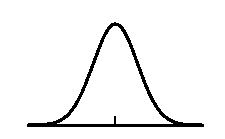
\includegraphics[]{gauss}
  \label{fig:gaussian}}
\subfigure[]{
  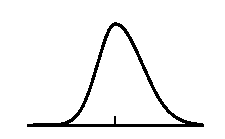
\includegraphics[]{asym02}
  \label{fig:asym02}
}
\subfigure[]{
  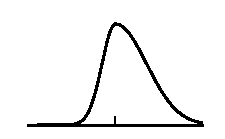
\includegraphics[]{asym04}
  \label{fig:asym04}
}
\subfigure[]{
  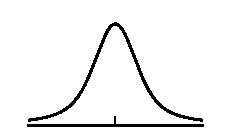
\includegraphics[]{voigt}
  \label{fig:voigt}
}
\subfigure[]{
  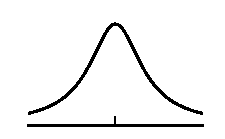
\includegraphics[]{lorentz1}
  \label{fig:lorentzian}
}
\subfigure[]{
  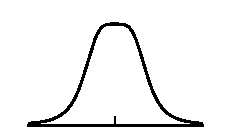
\includegraphics[]{lorentz2}
  \label{fig:lorentzian_flat}
}
\caption{QDOAS can use different line shapes to describe the
  instrumental slit function.  The plots above illustrate the
  Gaussian~(a), asymmetrical~(b, c), Voigt~(d) and Lorentzian~(e,~f)
  profile shapes.  The asymmetry factor in (b) is 0.2, that of line
  shape (c) is 0.4.  The Lorentzian (e) is the standard Lorentzian
  ($n=1$) and the Lorentzian in (f) has $n=2$.}\label{fig:lineshapes}
\end{figure}

\textbf{As a convention, QDOAS always requests the full width at half
  maximum (FWHM) of the line shape in the user interface.  This
  parameter is represented by $\sigma$ in the formulas below.}

\subsubsection{Gaussian}
The standard expression used to approximate instrumental slit
functions is the Gaussian function (see figure
\ref{fig:gaussian}). The Gaussian is the exact line shape in the
diffraction limit, i.e. in the case of an infinitely thin entrance
slit. The normalized Gaussian is given by
\begin{equation}
  \label{eq:gaussian}
  G_\sigma(x) =  \frac{1}{a\sqrt{\pi}}\exp\left(-\frac{x^2}{a^2}\right)\,,
\end{equation}
where $a$ depends on the Gaussian full width at half-maximum $\sigma$ as follows:
\begin{equation}
  \label{eq:gaussian_fwhm}
  \sigma = 2\sqrt{\ln 2}a\,.
\end{equation}

\subsubsection{Error function}
For a large entrance slit, the slit function can be approximated by
the convolution of a boxcar and a Gaussian function.  The resulting
slit function is given by
\begin{equation}
  \label{eq:error_function_slit}
  E_a(x) = \frac{1}{4\Delta}\left(
    \mathrm{erf}\left(\frac{x+\Delta}{a}\right) - \mathrm{erf}\left(\frac{x-\Delta}{a}\right) \right)\, ,
\end{equation}
where $a$ depends on the Gaussian full width at half-maximum $\sigma$ (see \ref{eq:gaussian_fwhm}),
$\Delta$ is half the boxcar width $b$ and $\mathrm{erf}(x)$ is the
error function, defined by
\begin{equation}
  \label{eq:error_function}
  \mathrm{erf}(x) = \frac{2}{\sqrt{\pi}}\int_0^x \exp(-t^2)\mathrm{d}t\,.
\end{equation}

Full width at half maximum of the Gaussian $\sigma$ (see
\ref{eq:gaussian_fwhm}) and boxcar width $b$ (2*$\Delta$) are the two
parameters requested by QDOAS for the error function.

\subsubsection{2$n$-Lorentzian}
This line shape is a generalization of the well-known Lorentzian
function ($n=1$, see figure \ref{fig:lorentzian}).  It is useful to
approximate slit functions with a shape significantly different from
the Gaussian one. Low order 2$n$-Lorentz can mimic line shapes with
large wings (typically the standard Lorentzian profile), or line
shapes having a flat top (for higher values of $n$, see figure
\ref{fig:lorentzian_flat}). The generic expression for this function
is
\begin{equation}
  \label{eq:2nlorentz}
  L_{2n}(x) = \frac{\tau^{2n}}{x^{2n}+\tau^{2n}}\,,
\end{equation}
with $\tau=\sigma/2$ ($\sigma$ is the full width at half maximum).

Parameters requested by QDOAS are the full width at half maximum
$\sigma$ and the parameter $n$, called ``Order''.

\subsubsection{Voigt profile}
The Voigt profile function (see figure \ref{fig:voigt}) is the
convolution of a Gaussian and a Lorentzian function. This function is
used in a wide range of contexts, and the optimization of its
computation has received much attention. The Voigt profile is usually
expressed as
\begin{equation}
  \label{eq:voigt_profile}
  K_(x,y) = \frac{y}{\pi} \int_{-\infty}^{\infty} \frac{\exp(-t^2)}{(x-t)^2+y^2}\mathrm{d}t\,,
\end{equation}
where $x$ is the distance from the line center in units of Gaussian
half-widths and $y$ is the ratio of the Lorentzian width to the
Gaussion width. Numerous ways have been proposed to compute the Voigt
function. A rather efficient algorithm is described
by~\citet{Kuntz_1997}. % is this the algorithm used in QDOAS?

\subsubsection{Asymmetrical Gaussian}
To handle asymmetrical line shapes, QDOAS can fit an asymmetry factor
in addition to the \gls{fwhm}.  The line shape used is a modified version of
the Gaussian line shape (\ref{eq:gaussian})
\begin{equation}
  \label{eq:asymmetrical_line}
  G'(x) = \frac{1}{a\sqrt{\pi}}\exp\left(
    -\frac{x^2}{a^2(1+\mathrm{sign}(x)b)^2}\right)\,,
\end{equation}
where, in addition to the FWHM $\sigma$, the asymmetry factor $b$ is
now fitted as well.  For a value of $b=0$, it reduces to the ordinary
Gaussian line shape.  Figure \ref{fig:asym02} illustrates the line
shape with an asymmetry factor of $b=0.2$ and \ref{fig:asym04} gives
an illustration for $b=0.4$.

\subsubsection{Super Gaussian}
This line shape is a generalization of the Gaussian with the introduction of two independent parameters, w and k, determining
the width and shape of the slit function.  This line shape has been the subject of studies by Steffen Beirle from the Max-Planck Institute in Germany and summarized in a recent paper (\citep{Beirle2017}).
The current implementation in QDOAS is operational but not optimized in terms of performance.

\subsection{User-defined line shape}\label{sec:userdef-line-shap}

An alternative to fit asymmetrical slit functions is to provide a line shape in an ASCII file and to apply on the grid of the line shape a stretch factor that can be different for each side of the line shape.
The ``Stretch on wavelength'' file in the \textbf{Convolution tool} is a ASCII file with three columns : the wavelength calibration and the two values of the stretch to apply on the grid of the line shape for each wavelength of the detector.

Lookup tables of slit functions are also accepted.  This means that a
line shape is provided for different wavelengths.  For a specific
wavelength, a line shape is first calculated by linear
2D-interpolation in the lookup table and the fitted stretch factors
are then applied to the line shape wavelength grid before convolution.

\subsection{Wavelength dependency}
QDOAS supports convolution with wavelength-dependent slit functions:
\begin{itemize}
\item Slit function files provided by the user may contain multiple
  columns describing the shape of the slit function at various
  wavelengths.  The first line of the file should list the wavelengths
  for which the slit function is provided.  QDOAS will then generate a
  lookup table from the provided slit functions, and calculate the
  slit function at intermediate wavelength values using linear
  interpolation.
  % explain this in more detail (and perhaps move this to the tools or
  % properties chapters?)
\item For analytical line shapes, the user can provide a two-column
  ASCII file containing the wavelengths and corresponding values of
  the parameters for each requested parameter (for example, the
  Gaussian width and the boxcar width for the error function).  Files
  with the correct parameter calibration can be saved from the SFP
  plots obtained after the wavelength calibration procedure.
\end{itemize}
For more details on how to compute such a convolution using QDOAS, see
section \ref{sec:conv-tool}, page \pageref{sec:slit-function-page}.

\subsection{Correction for the Solar $I_0$-effect}\label{sec:correction-solar-i_0}
The $I_0$-effect is due to the difference between cross sections
measured in the laboratory with a smooth light source and the
atmospheric absorption measured by an instrument of lower resolution
with a structured solar light source~\citep{aliwell_2002}.  As
described in equation~\eqref{eq:optical_density}, the DOAS technique
attempts to isolate the atmospheric absorptions by calculating the
ratio of a reference spectrum $I_0$ and a measured spectrum $I$.
However, because the two spectra in this ratio have been filtered by
the instrument function before the calculation of the ratio, complete
removal of the Fraunhofer structure from the solar reference spectrum
is not possible:

If the $I_0$-effect is not accounted for, the cross sections $S$ used
in the DOAS retrieval are laboratory cross sections $S_0$ convolved
with the instrumental slit function $F$:
\begin{equation}
  \label{eq:cross_section_convolved}
  S(\lambda) = (F\ast S_0)(\lambda) = \int S_0(\lambda') F(\lambda-\lambda')\mathrm{d}\lambda' \,.
\end{equation}
The intensities measured by the spectrometer can be defined as
\begin{align}
  \label{eq:incoming_intensity}
  I_0^{\mathrm{meas}}(\lambda) &= (F\ast I_0)(\lambda)\,,\\
  I^{\mathrm{meas}}(\lambda) &= (F\ast I)(\lambda) = \left( F \ast I_0 \exp(-S_0 \cdot c)\right)(\lambda)\,.
\end{align}
Taking into account the instrumental function $F$,
equation~\eqref{eq:optical_density} becomes:
\begin{align}
  \tau = \ln \frac{I_0^{\mathrm{meas}}(\lambda)}{I^{\mathrm{meas}}(\lambda)}
  &  = \ln \frac{ (F \ast I_0)(\lambda)}{ (F \ast I_0 \exp(-S_0 \cdot c))(\lambda)}\\
  & \simeq c \cdot (F * S_0)(\lambda)\,. \label{eq:convolution_approximation}
\end{align}
Thus, the fitting of convolved laboratory cross sections to the
optical depth measured by a low resolving instrument relies on an
approximation.  The error induced by this approximation depends on the
absorption strength and the relation between the width of the slit
function and the width of the spectral structures in the light source
$I_0$ and the cross section $S_0$.  For most of the atmospheric
absorbers the $I_0$-effect is negligible but in some cases, the
approximation (\ref{eq:convolution_approximation}) is not accurate
enough. This is particularly the case for strong atmospheric absorbers
such as \ozone{}.

This effect may be dealt with to a good approximation by correcting
the laboratory cross sections with the solar Fraunhofer spectrum: for
a particular absorber, a highly resolved solar spectrum $I_0(\lambda)$
and a simulated absorption spectrum $I^*_c(\lambda)$ with a known slant
column $c$ are both convolved with the instrument slit function
\begin{align}
  I_0^*(\lambda)&= (F \ast I_0) (\lambda)\, ,\\
  I^*_c (\lambda) &= (F \ast I_0 \exp( -S_0 \cdot c)) (\lambda)\,.
\end{align}
The $I_0$-corrected cross section $S*$ is then defined by
\begin{equation}
  \label{eq:I0_corrected_cross_section}
  S^*_c(\lambda) = -\frac{1}{c}\ln \left(
    \frac{ I^*_c(\lambda) }{I^*_0(\lambda)}
  \right)\,.
\end{equation}
The $I_0$-corrected cross section derived in this manner perfectly
matches the absorptions in the measured atmospheric spectrum, provided
that the SCD $c$ used in the calculation is equal to the true
atmospheric SCD. However, this is not a critical point and the $I_0$
corrected cross sections can be used for a large range of atmospheric
slant column densities~\citep{Wagner1999}.

\subsection{Deconvolution}\label{sec:deconvolution}
The QDOAS convolution tool implements a de-convolution option. In this
case, the convolution is performed using an effective slit function
obtained after Fourier transform manipulation of specified convolution
and de-convolution functions. The effective slit function is
calculated as follows:
\begin{equation}
  \label{eq:deconvolution}
  S_{\mathrm{eff}} = \mathfrak{I}^{-1} \left[
    \frac{ \mathfrak{I}(S_1) }{\mathfrak{I}(S_2)}
    \right]\,,
\end{equation}
$\mathfrak{I}$ represents the Fourier transform, and $S_1$ and $S_2$ are
respectively the convolution and de-convolution slit functions. Great
care is taken in the algorithm to avoid noise-corruption effects when
taking the ratio of the Fourier transforms.

%%% Local Variables:
%%% mode: latex
%%% TeX-master: "QDOAS_manual"
%%% TeX-PDF-mode: t
%%% End:

\chapter{Quick start} \label{cha:quickstart}

This chapter guides you step by step towards the complete configuration of a project using a predefined
configuration provided with the package (setup for \NO2 retrieval from ground-based \glslink{maxdoas}{MAXDOAS} measurements).
The retrieval settings are those recommended during the \glslink{cindi}{CINDI} intercomparison campaign (see \citet{Roscoe2010}).

\section{Creating a project to browse spectra}

\subsection{Creating a New Project}

When QDOAS starts on an empty application, the user interface looks like~:

\hfill\vspace{-.8\baselineskip}
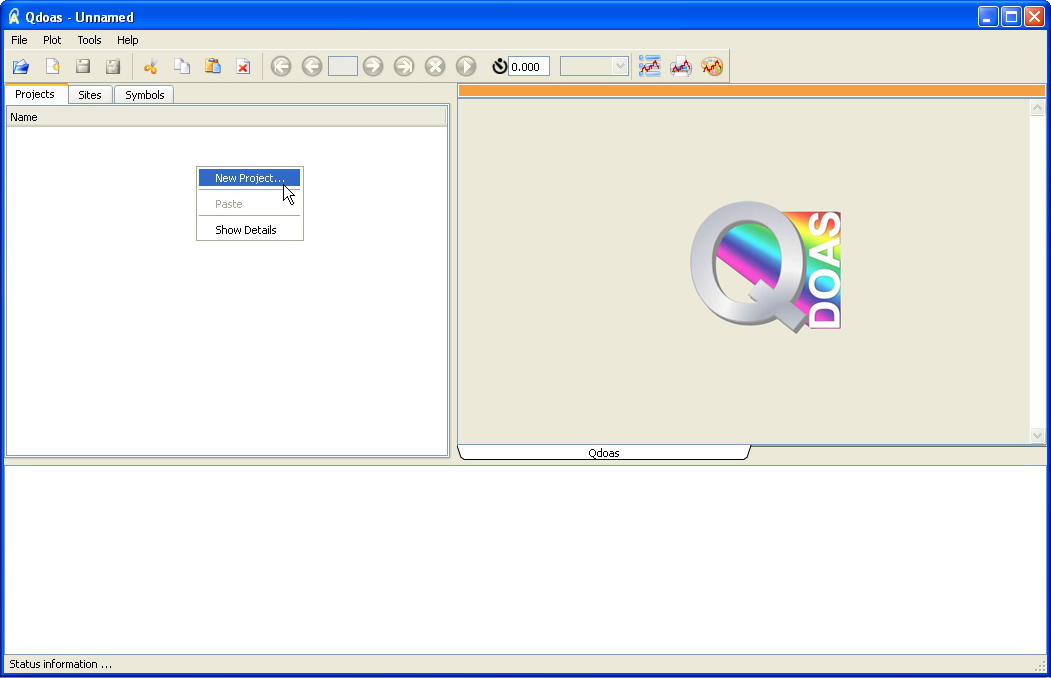
\includegraphics[width=\textwidth]{img/Quickstart_New.jpg}

From the upper-left panel, right-click the \textbf{New Project} option, and give it a name, for example MAXDOAS-VIS
as the purpose of the application here is to retrieve \NO2 from MAXDOAS measurements in the visible region.

\begin{minipage}{\textwidth}
\subsection{Project properties}
\hfill\vspace{-.8\baselineskip}
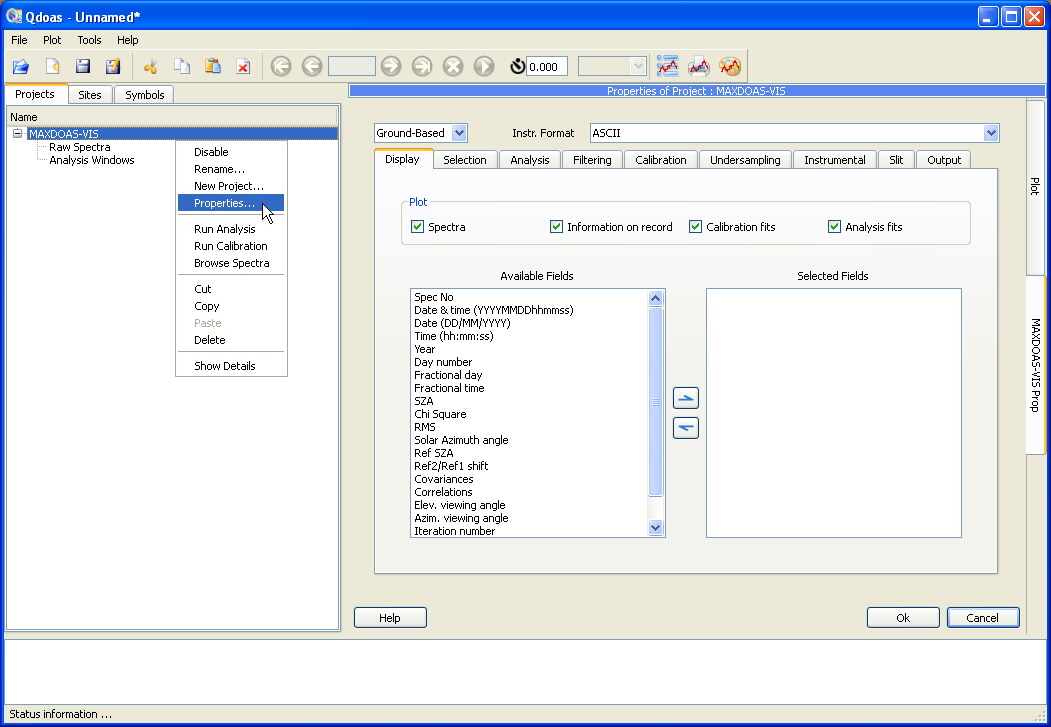
\includegraphics[width=\textwidth]{img/Quickstart_ProjectProperties.jpg}
\end{minipage}\\

From the MAXDOAS-VIS tree node, right-click \textbf{Properties} to open the \textbf{Properties} dialog box on the upper-right panel.
Switch to the \textbf{``Instrumental"} page to complete information on the format of the files to read.  The default file format
(\textbf{Ground-based, ASCII}) is correct for the example~:

\hfill\vspace{-.8\baselineskip}
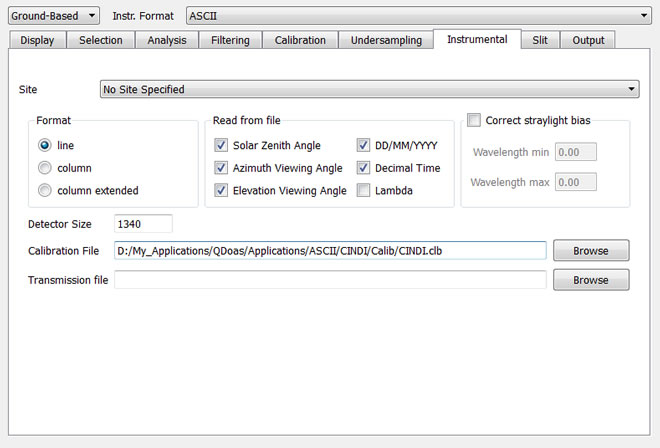
\includegraphics[width=\textwidth]{img/Quickstart_ProjectInstrumental.jpg}

The detector size has to be specified.  The files in the example contain one  record per line and the following information are given in the expected order~:

\begin{minipage}[t]{\textwidth}
\vspace{-1\baselineskip}
\begin{itemize} \itemsep -6pt
\item Solar Zenith Angle
\item Azimuth Viewing Angle
\item Elevation Viewing Angle
\item Date in the DD/MM/YYYY (day/month/year) format
\item Fractional time
\end{itemize}
\end{minipage}
\vskip 6pt

The wavelength calibration is provided in a separate file.

Switch back to the \textbf{``Display"} page to select information you want to see when browsing spectra and click ok to save \textbf{Projects properties}~:

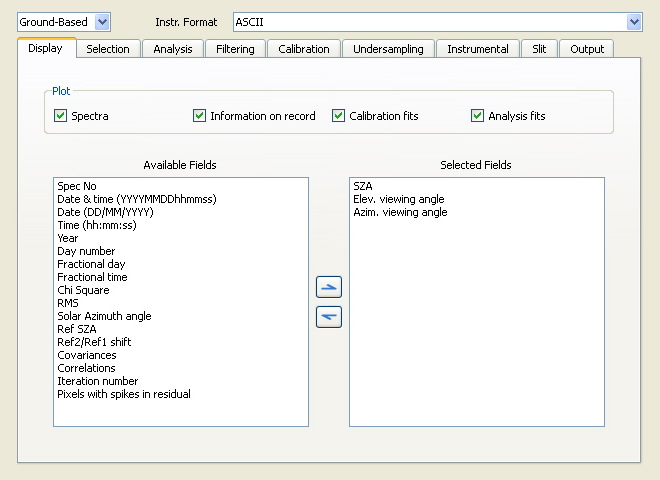
\includegraphics[width=\textwidth]{img/Quickstart_ProjectDisplay.jpg}

\subsection{Inserting Files}

To insert files under the new project, right-click \textbf{Insert File} or \textbf{Insert Directory} from the \textbf{Raw Spectra} node.
We prefer to select the directory~:

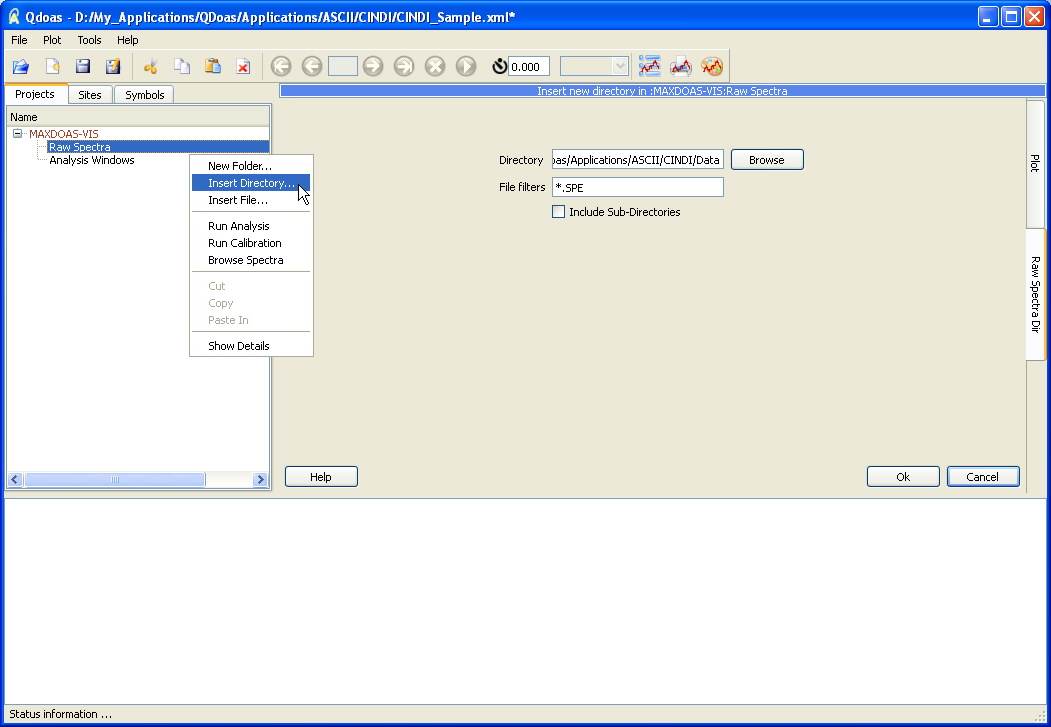
\includegraphics[width=\textwidth]{img/Quickstart_InsertFiles.jpg}

\subsection{Browsing Files}

Right-click the \textbf{Browse Spectra} option from the \textbf{Data directory} name to browse spectra ~:

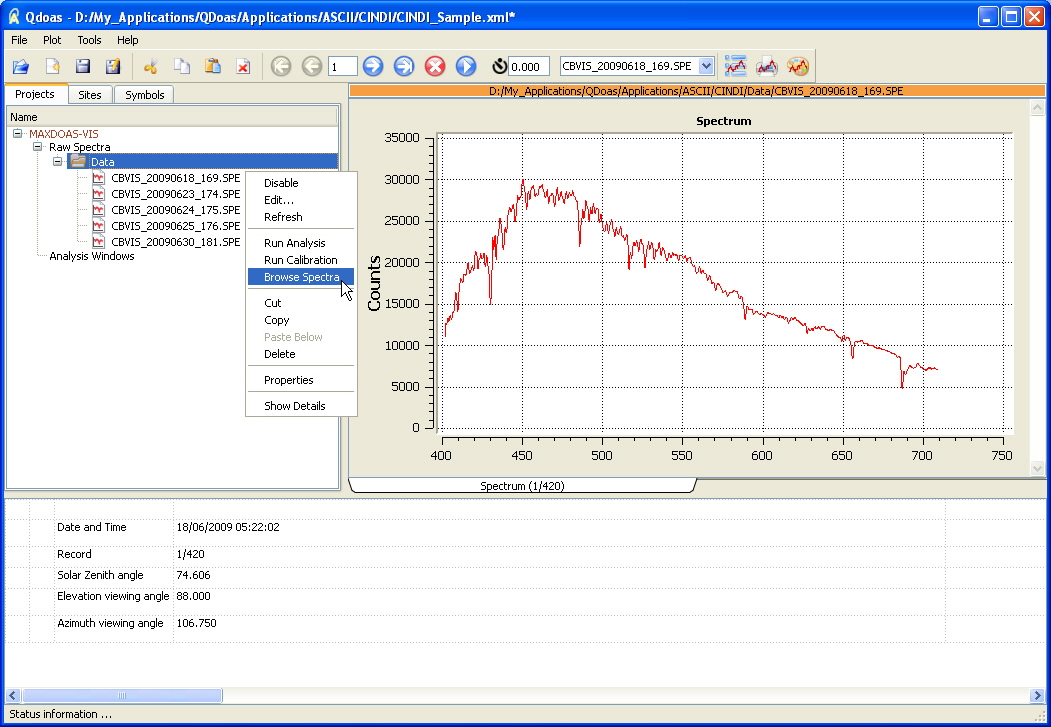
\includegraphics[width=\textwidth]{img/Quickstart_BrowseSpectra.jpg}

Buttons of the toolbar allow moving from one record to the other but also to switch to another file of the directory (possible if the
\textbf{Browse spectra} option has been clicked from the root directory and not from a file).


\subsection{Handling Graphs}

Zoom is possible by right-clicking the \textbf{Interactive} option from the \underline{\textbf{plot title}}~:

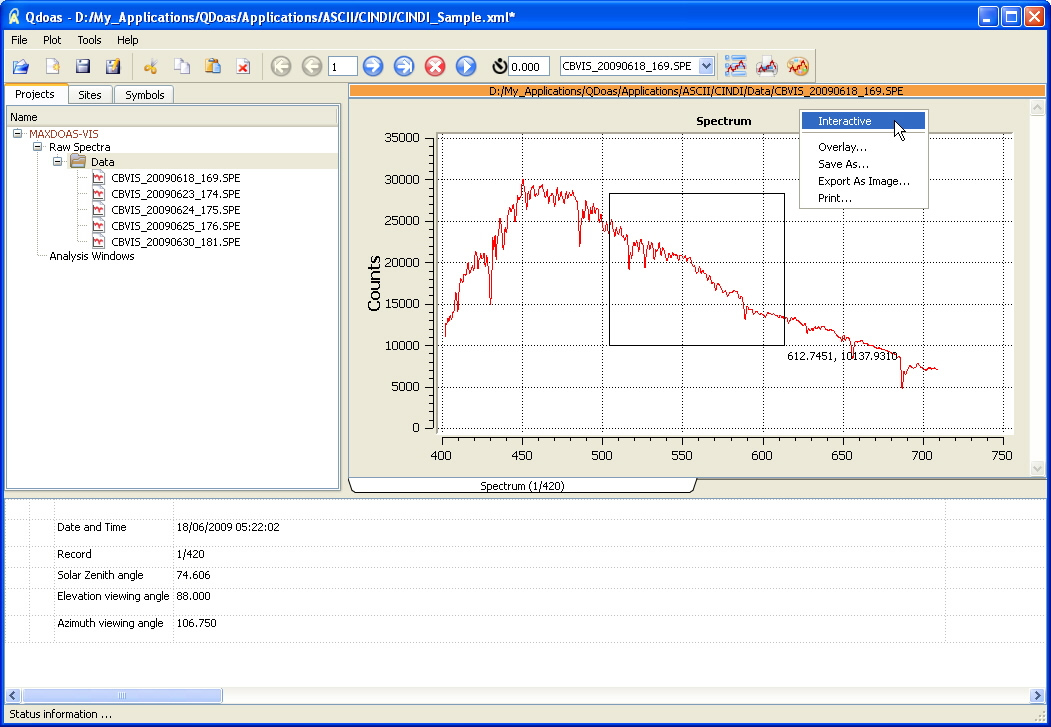
\includegraphics[width=\textwidth]{img/Quickstart_PlotZoom.jpg}

Other options such as export the plot in ASCII (\textbf{Save As}) or PNG (\textbf{Save As Image}) are also available.  Reference spectra used in the retrieval can be saved in ASCII by this way.

\subsection{Saving Your Work}

Be sure to save your work regularly using \textbf{File $\rightarrow$ Save} or  \textbf{File $\rightarrow$ SaveAs}.
The format of configuration files is XML.  Always use the \textbf{Stop} button (cross in a red circle) in the toolbar before coming back
to the project configuration.

\section{Example~: Configuration of a project for \NO2 retrieval}

\subsection{Configuring A Project For Spectra Analysis}

The configuration of a project requires the following steps~:

\begin{qdoasitem}
\item define all symbols related to the cross sections files that will be used in the analysis;
\item call back the \textbf{Projects properties} dialog box to parameterise the wavelength calibration procedure and to setup analysis options independent of the spectral window (fitting method, unit for shifts);
\item create an \textbf{`Analysis Window'} item in the \textbf{Projects} tree for each spectral window to process, and parameterise it.
\end{qdoasitem}

These steps are described through the example file \textbf{CINDI\_Sample.xml} provided with the package.

\subsection{Description of CINDI\_Sample.xml}

The file \textbf{CINDI\_Sample.xml} contains the configuration of a project for \NO2 retrieval.
Before using the file, you may change the paths according to your installation.  The fastest way to do it is to
edit the file and replace all \textbf{D:/My\_Applications/QDoas/Applications/ASCII/CINDI} according to your installation.
Then, use \textbf{Files $\rightarrow$ Open} command from the QDOAS menu bar or the equivalent button in the toolbar to load the application.

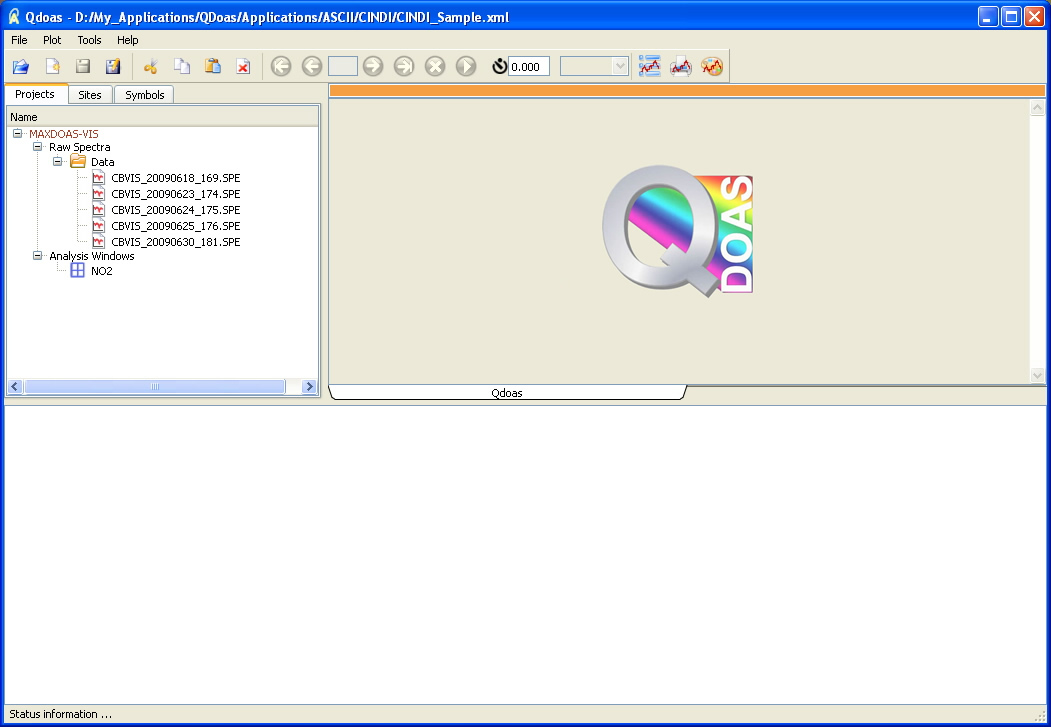
\includegraphics[width=\textwidth]{img/Quickstart_Project.jpg}

\subsection{Settings For NO$_{2}$ Retrieval} \label{sec:no2_settings}

\textbf{Calibration interval}~: depends on the wavelength range covered by the detector.  It should include all spectral windows.
In our application, we have selected 405-580 nm.  A preliminary calibration has been previously measured in laboratory and already
improved with the wavelength calibration procedure of QDOAS (see section \ref{sec:wavel-calibr})

\textbf{Spectral window}~: 425-490 nm;

\textbf{Main Cross sections}~:

%\hfill\vspace{.8\baselineskip}
\begin{longtable}{ l p{6cm} l }
     & \textbf{Source} & \textbf{Files} \\
   \textbf{O$_3$} & \citet{Bogumil2003}, 223 K	& o3\_223K\_Bogumil.xs \\
	  \textbf{NO$_2$}	& \citet{vandaele1996}, 298 K et 220 K	& no2\_298K\_vanDaele.xs \\
   & & no2a\_220K\_vanDaele.xs \\
	  \textbf{O$_4$} & Hermans et al.	& o4\_Hermans\_web.xs\\
	  \textbf{H$_2$O} & From HITRAN data base	& h2o\_hitran.xs \\
	  \textbf{Ring} &	Ratio of the rotational raman spectrum by the solar one,  both convolved at the resolution of the instrument with the \textbf{Convolve Ring} option.	& Ring\_NDSC2003.xs
\end{longtable}

The cross sections are those recommended during the \glslink{cindi}{CINDI} intercomparison campaign (see \citet{Roscoe2010}).

\subsection{Defining Symbols}

The first thing to do is to define the cross sections symbols according to the files names (see table above)~: O3, NO2, NO2a, O4, H2O, Ring
(the case is not important).  A description can be added.  QDOAS needs these symbols for internal use.

\begin{center}
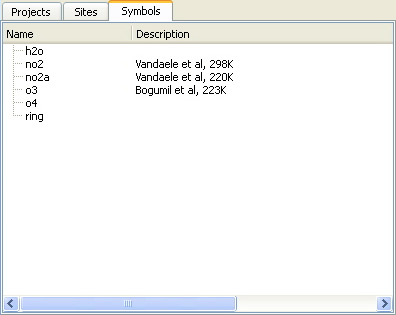
\includegraphics[scale=0.5]{img/Quickstart_Symbol.jpg}
\end{center}

\begin{minipage}{\textwidth}
\subsection{Projects Properties}\hfill
\vspace{-0.8\baselineskip}
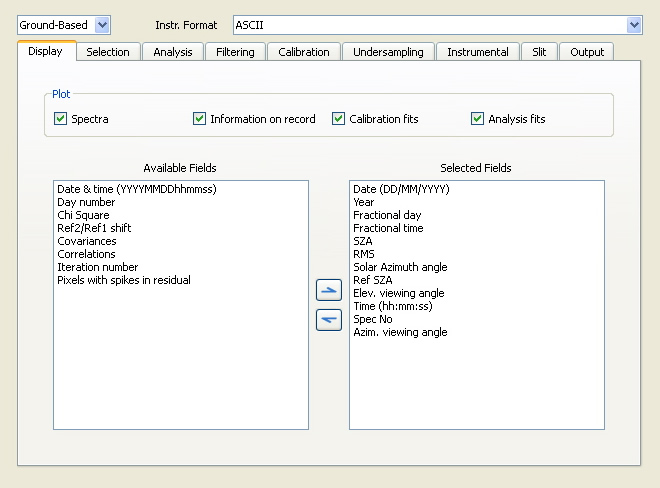
\includegraphics[width=\textwidth]{img/Quickstart_DisplayPage.jpg}
\end{minipage}

Go back to the \textbf{Projects tree} and right-click the \textbf{Properties} command from the MAXDOAS-VIS
node to open the \textbf{Projects properties} dialog box.  The \textbf{Display} tab page appears first.
Some additional fields related to the analysis can be selected such as the  \glslink{rms}{\textbf{RMS}} or the reference spectrum \gls{sza} (\textbf{Ref SZA})~:

\subsubsection{Calibration Parameterisation}\label{sec:calibr-param}
In the example, the \textbf{Calibration} page is configured as follows~:

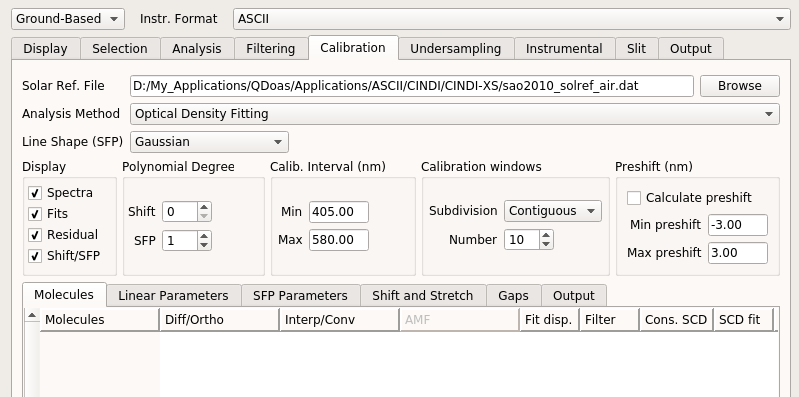
\includegraphics[width=\textwidth]{img/Project_Calibration.png}

\begin{description}
\item[Solar ref. file] Use this button to locate the solar spectrum
  (in this case, a high-resolution one because the slit function is
  fitted, otherwise a solar spectrum previously convolved at the
  resolution of the instrument).
\item[Analysis Method] The fitting method used for wavelength
  calibration can be different from the one selected for spectra
  evaluation in the \textbf{Analysis tab page}.
\item[Line Shape (SFP)] This button is checked in order to fit the
  resolution of the slit function; in this case, a Gaussian line shape
  is selected.
\item[Display] Check boxes in the frame to display the indicated
  graphs.
\item[Polynomial degree] The degree of the polynomial used in the
  final determination of the wavelength registration (shift) and the
  wavelength-dependent slit function (SFP).
\item[Calib.\ Interval (nm)] The complete calibration interval.
\item[Calibration windows] The number of calibration subwindows, as
  well as settings to control their position within the calibration
  interval.
\end{description}

Options are also distributed in several pages.  The four following ones are the most important for the wavelength calibration.

\subsubsection{Molecules}
\hfill\vspace{-.8\baselineskip}
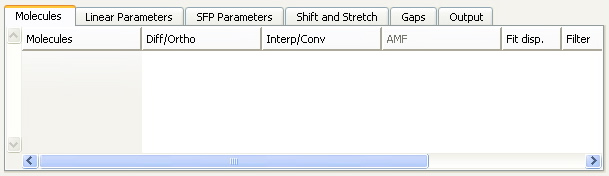
\includegraphics[width=\textwidth]{img/Quickstart_CalibrationMolecule.jpg}

In this page, we can specify absorption cross sections to include in
the fitting procedure (absorbing correcting terms).  For best results
(and given the usually limited information content within individual
sub-windows), it is recommended to limit the number of parameters.  In
our example, we do not include cross sections in the fit.  In the UV
region, it is sometimes necessary to add Ring and ozone.  In this
case, proceed as follows.  First try and fit the cross section term(s)
freely, looking at the retrieved values in each interval.  The usual
situation is that spectral signatures are such that the information
content largely differs from one interval to another.  Look at results
in the `best windows', and fix the absorber amount to a mean value
derived from these particular intervals.  Although this way of working
implicitly assumes that the molecule absorption is constant over the
whole calibration interval (which is not necessarily true), this is
usually the best compromise.

\begin{minipage}{\textwidth}
\subsubsection{Linear Parameters}
\hfill\vspace{-.8\baselineskip}
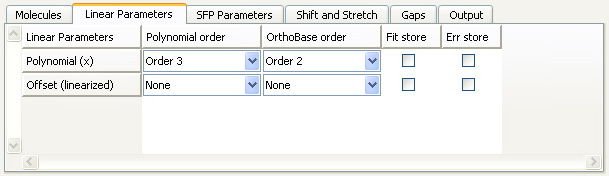
\includegraphics[width=\textwidth]{img/Quickstart_CalibrationLinear.jpg}
\end{minipage}\\

The smooth component of the differential absorbance is fitted by a polynomial.  The degree of the polynomial may be adjusted according
to the size of sub-windows and the quality of the fit.  The orthogonal base is used to calculate differential cross sections (not present
in this example).

\begin{minipage}{\textwidth}
\subsubsection{SFP Parameters}
\hfill\vspace{-.8\baselineskip}
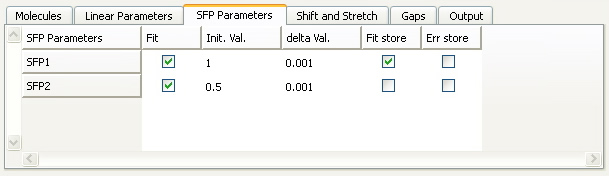
\includegraphics[width=\textwidth]{img/Quickstart_CalibrationSFP.jpg}
\end{minipage}
\glspl{sfp} are defined in this page.

In the example, the selected line shape is a gaussian.  The parameter
to fit is the \gls{fwhm} which is represented by SFP1.  The other
parameter SFP 2 is ignored for this type of line shape even though it
is checked.

Again in this case, a better accuracy is obtained when limiting the number of free parameters according to the information
content of spectra.  For line shapes involving two parameters such as the error function, which is the convolution between
a Gaussian (SFP 1) and a boxcar (SFP 2), it is recommended to fix the value of one (or several) parameters in order to optimize
the algorithm.  Several iterations may be needed.

\begin{minipage}{\textwidth}
\subsubsection{Shift and Stretch}
\hfill\vspace{-.8\baselineskip}
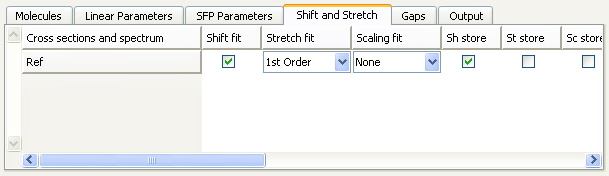
\includegraphics[width=\textwidth]{img/Quickstart_CalibrationShift.jpg}
\end{minipage}

Shift (and stretch) can be applied either on the control spectrum
(symbol \textbf{Spectrum} in this case) or on the solar spectrum
(symbol \textbf{Ref} in this case).  In order to avoid interpolating
the control spectrum, we recommend to shift the high-resolution solar
spectrum instead of the control one (see equation \ref{eq:gaussian},
section \ref{sec:wavel-calibr}).  \emph{Note that, in this case, the
  cross section(-s) defined in the \textbf{Molecules} page must be
  shifted together with the solar spectrum.}

Right-click the \textbf{Insert} or \textbf{Modify} option to add a new item in the list or to modify a selection.

\subsection{Analysis Window Properties}
To create a `new Analysis Windows' item in the \textbf{Projects} tree, select the predefined
\textbf{`Analysis Windows'} node (or an existing analysis window to add the new one after) and right-click
the \textbf{``New Analysis Windows..."} command.  Give it a name and right-click the properties option from the new
analysis windows item to have the following dialog box.

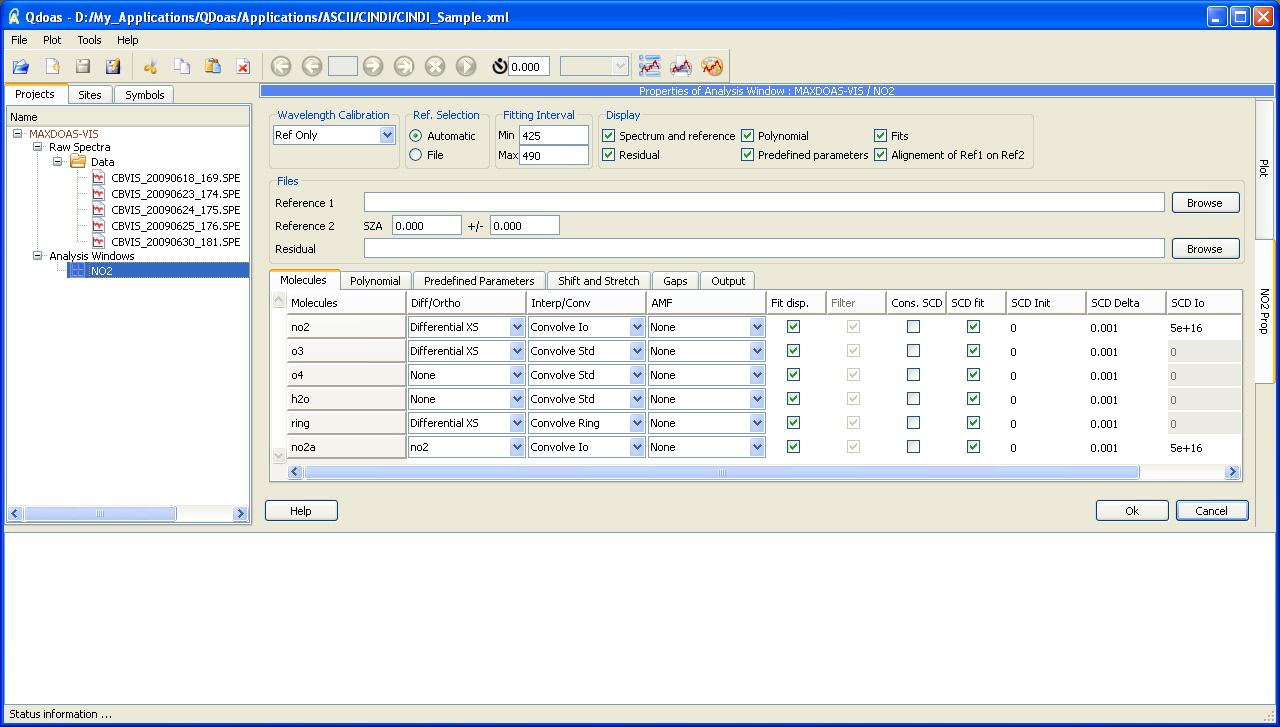
\includegraphics[width=\textwidth]{img/Quickstart_Analysis.jpg}

\subsubsection{Analysis Windows Properties}

The recommended \textbf{fitting interval} for \NO2 in the visible region is 425-490 nm.

We have checked the option \textbf{Automatic} in the \textbf{Reference selection} frame.  This means that a reference spectrum is automatically selected every day from the current data file.  If both values are not zero, the spectrum will be different for each twilight.  In the example, the spectrum measured at the minimum solar zenith angle of the day is selected.

The wavelength calibration is applied on the reference spectrum (here, \textbf{Reference 2}).  If a file had also been specified in \textbf{Reference 1}, it would have had  the priority for the wavelength calibration and the shift between both \textbf{Reference 1} and \textbf{Reference 2} would have been determined in order align cross sections on \textbf{Reference 2} before the analysis of spectra.

The structure of the \textbf{Analysis Windows Properties} pages is very similar to the one used for the calibration (and already defined above).

\subsubsection{Molecules}
\hfill\vspace{-.8\baselineskip}
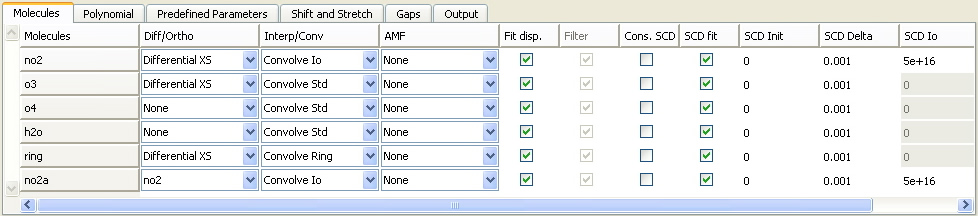
\includegraphics[width=\textwidth]{img/Quickstart_AnalysisMolecules.jpg}

This page contains the absorption cross sections needed for \NO2 retrieval (see the list, page \pageref{sec:no2_settings}).  Differential cross sections
are generated by orthogonalisation to an orthogonal base defined in the \textbf{Polynomial} page.  In order to avoid correlation between cross sections
(e.g. NO2 and NO2a) of similar shapes (e.g. when treating temperature effects by including two or several cross sections of the same species),
these cross sections can be orthogonalised with respect to each other.  High-resolution cross sections are convolved using the information
on the calibration and the slit function retrieved from the wavelength calibration procedure.  \NO2 cross sections are convolved using $I_0$ correction
(see page \pageref{sec:no2_settings}); a typical concentration of $5e16$ is used.

\subsubsection{Polynomial}
\hfill\vspace{-.8\baselineskip}
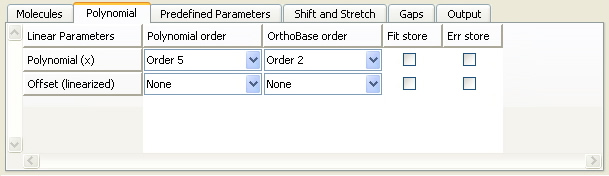
\includegraphics[width=\textwidth]{img/Quickstart_AnalysisLinear.jpg}

In this page, the polynomial used for fitting the smooth part of the absorbance is defined.  An orthogonal base is built with the main components of the polynomial in order to calculate differential cross sections.

\subsubsection{Predefined Parameters}
\hfill\vspace{-.8\baselineskip}
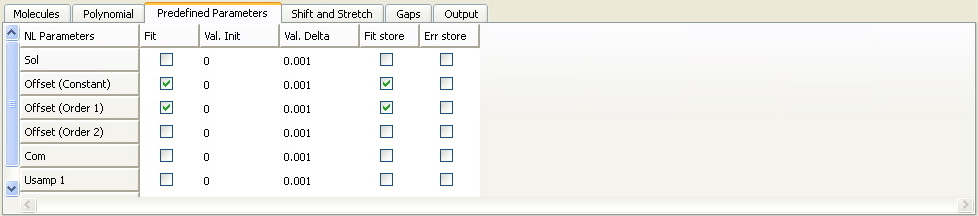
\includegraphics[width=\textwidth]{img/Quickstart_AnalysisPredefined.jpg}

Predefined parameters page contains reserved symbols not defined by the user (for example, offset).

\subsubsection{Shift and Stretch}
\hfill\vspace{-.8\baselineskip}
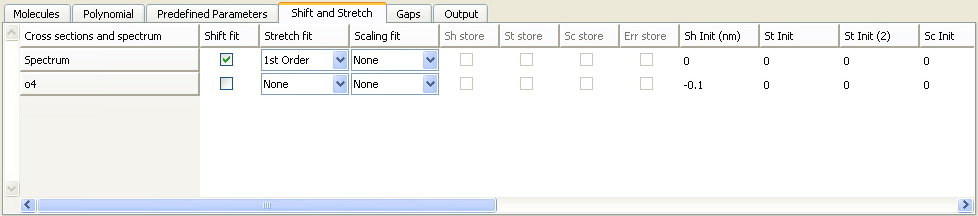
\includegraphics[width=\textwidth]{img/Quickstart_AnalysisShift.jpg}

Shift and stretch (1st order) applied to the spectrum are fitted here.  In this page, a shift value is also applied (not fitted) to the \tetraox~cross section.  Note that several cross sections can be grouped together.  Right-click the \textbf{Insert} or \textbf{Modify} option to add a new item or to modify the selection.

\subsection{Running Analysis}

To analyse a spectra file, select it in the \textbf{Projects} tree and right-click the \textbf{Run Analysis} command.

\begin{tabular}{p{1.5cm} p{10cm}}
\textbf{Note}	& if you right-click \textbf{Run Analysis} command from a parent node (\textbf{Data} folder or \textbf{Raw Spectra}), the command will be applied on all spectra files defined in the selected project.
\end{tabular}

The analysis of a record is processed in one shot (even if several analysis windows are defined) and the results of the fit are plotted in different pages.  The panel at the bottom of the user interface provides information related to the type of plot currently displayed.

\begin{minipage}{\textwidth}
\subsubsection{Kurucz page}
\hfill\vspace{-.8\baselineskip}
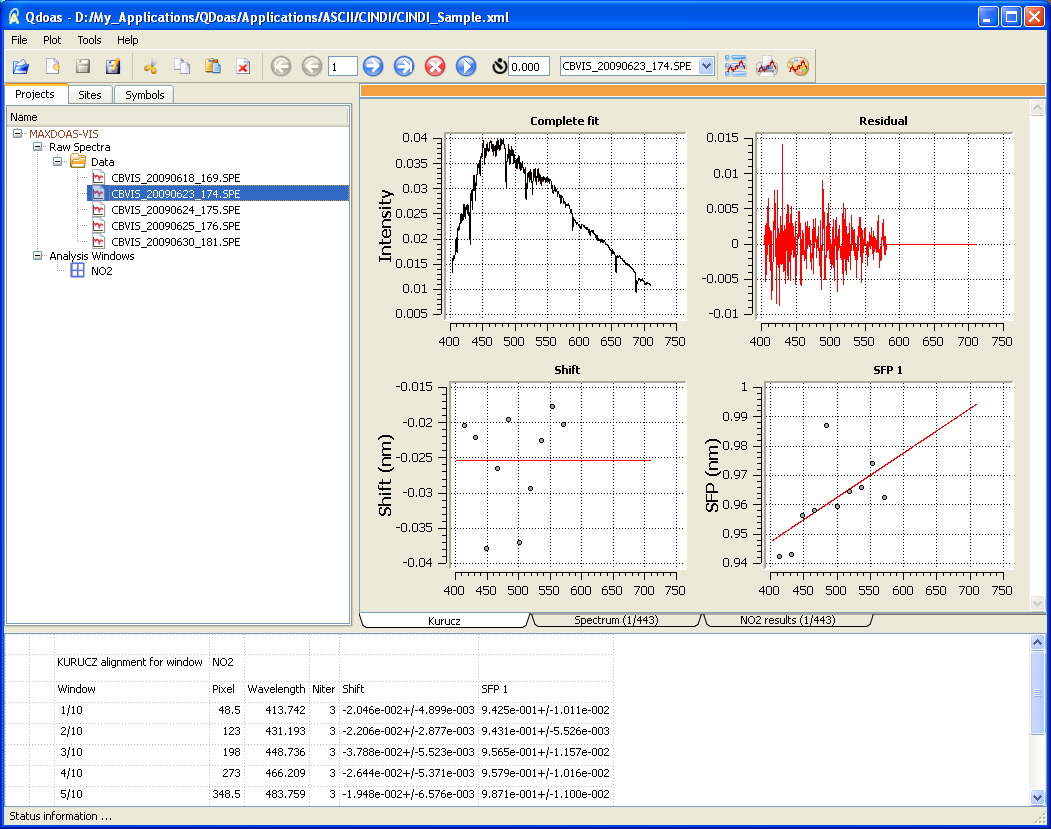
\includegraphics[width=\textwidth]{img/Quickstart_RunAnalysis.jpg}
\end{minipage}\\

This page appears in front of the others when the first spectrum is processed.  It contains the plots resulting from the wavelength calibration procedure~:

\begin{qdoasitem}
\item \textbf{Complete fit}~: the selected reference spectrum (in red) is compared to the high-resolution solar spectrum convolved with the calculated resolution of the instrument (in black); if you zoom in the plot, you can check if structures match.  The wavelength calibration is the new calculated one.  It can be saved by right-clicking on the \textbf{Save As} option in order to be associated to another reference spectrum.
\item \textbf{Residual}~: the normalised residual;
\item \textbf{Shift}~: the calibration error;
\item \textbf{SFP 1}~: the variation of the \gls{fwhm} of the Gaussian with the wavelength.
\end{qdoasitem}

The red line represents the polynomial that fits individual points calculated in each sub-windows (black dots).  The whole detector wavelength range is covered.  All this information can be saved in a file using the \textbf{Save As} option.  A file with four columns is created (new wavelength calibration, polynomial fitting the individual points, wavelength at the centre of each sub-window and the calculated value for this sub-window.  Columns 3 and 4 are completed with "0" values in order to have the number of points of the detector.

\subsubsection{Spectrum page}

The currently analyzed spectrum is displayed in this page.  The panel at the bottom of the user interface provides information on the record according to the selection made in the \textbf{Selection page} of \textbf{Projects Properties}.

\subsubsection{NO2 page}
\hfill\vspace{-.8\baselineskip}
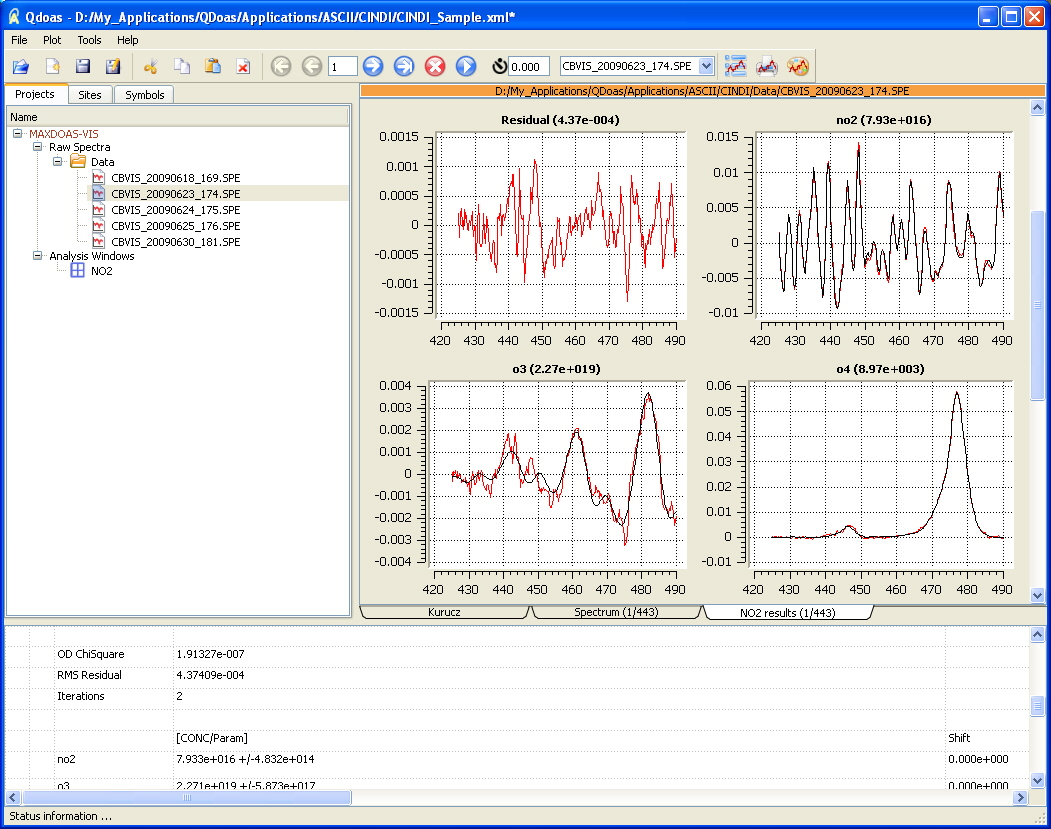
\includegraphics[width=\textwidth]{img/Quickstart_RunAnalysis_Fit.jpg}

The information on the calibration and the resolution of the instrument retrieved from the wavelength calibration procedure are used to convolve cross sections on the correct grid.   The cross sections respectively measured (the optical thickness after removal of the contribution of all molecules excepted one) and calculated (the remaining cross section multiplied by the calculated slant column density) are displayed.

\subsubsection{Output}
% add screenshot?
To save the results, stop the current analysis using the red button in the toolbar, open \textbf{Projects Properties}, and go to the \textbf{Output} page.  In order to save results, check ``Analysis'' and choose the location and format of the output file(-s).  Check ``Calibration'' to save reference spectrum calibration results as well.  Still on the \textbf{Output} page, you may select various other fields to be saved to the output file.  Next, go to the \textbf{Analysis Window Properties} to select molecule densities and other analysis results that should be saved to output.  To select which calibration data should be saved, go to the \textbf{Calibration} page of the \textbf{Projects Properties} window.

%%% Local Variables:
%%% mode: latex
%%% TeX-master: "QDOAS_manual"
%%% TeX-PDF-mode: t
%%% End:

\chapter{Projects and Analysis Windows Properties} \label{cha:properties}
This chapter covers:

\begin{enumerate} \itemsep -6pt
\item the configuration of projects;
\item the parameterisation of the analysis;
\item the parameterisation of the wavelength calibration.
\end{enumerate}

\section{Projects properties}\label{sec:projects-properties}
The \textbf{Projects properties} dialog box resumes the general options to configure the application.  These options are divided into the following categories:

\begin{longtable}[h]{l p{8cm}}
\textbf{Display}	& selection of information to display with spectra; \\ [6pt]
\textbf{Selection}	& selection of spectra to browse or to analyse; \\ [6pt]
\textbf{Analysis}	& options specific to the analysis (analysis method, interpolation, convergence criterion, \dots); \\ [6pt]
\textbf{Filtering}	& selection of a filtering method to apply on spectra and absorption cross sections; \\ [6pt]
\textbf{Calibration}	& configuration of the wavelength calibration procedure; \\ [6pt]
\textbf{Undersampling}	& selection of a method to calculate undersampling cross sections and to include them in the fit; \\ [6pt]
\textbf{Instrumental}	& options specific to the selected input file format; \\ [6pt]
\textbf{Slit} 	& definition of a slit function or a method to convolve cross sections before the analysis using the information generated by the wavelength calibration procedure; \\ [6pt]
\textbf{Output}	& selection of the information on the spectra that should be saved in the output file after the analysis. \\ [6pt]
\end{longtable}

The creation of a new project always starts with the definition of the measurement type (satellite, ground-based or airborne) and the selection of the spectra file format.

Before browsing spectra, options in the \textbf{Instrumental page} and in the \textbf{Display page} should be checked. Options in the other pages of the
\textbf{Project properties} concern the analysis of spectra and the configuration of the output. They have to be completed with the creation of cross sections
symbols and the settings in the \textbf{Analysis Windows properties} dialog boxes (definition of the spectral interval, specification of the reference spectrum,
selection of parameters to include or not in the \gls{doas} fit, \dots).

\begin{figure}[!h]
\subsection{Display Page} \label{sec:projects_display_page} \hfill
\vspace{-.8\baselineskip}
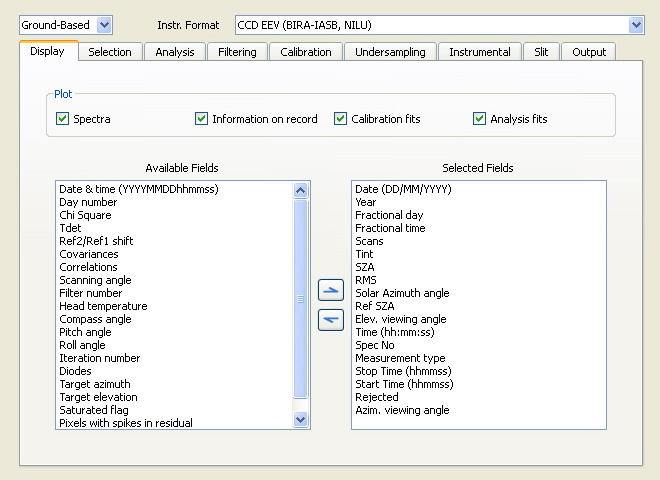
\includegraphics[width=\textwidth]{img/Project_Display.jpg}
\caption{Projects properties: Display page}\label{projects_properties_display}
\end{figure}
\FloatBarrier

The analysis of spectra can be performed in a non-stop way. Disabling the plot of spectra and fits during the analysis makes the processing significatively
faster although the use of the command line tool \textbf{doas\_cl} is recommended in this case. If the
\textbf{Spectra} button is unchecked, the state of the \textbf{Data} button has no effect.  If the \textbf{Calibration fits} button is unchecked, this will disable the display
of the calibration plots whatever the state of the buttons in the \textbf{Display frame} of the \textbf{Calibration page}.

\subsubsection{Selection Of Fields To Display}
The content of this frame is similar to the one in the \textbf{Output}
page. Information related to the measurements (e.g. date and time,
viewing angles, geolocation coordinates, \dots) can be selected in
this page and will be completed with analysis results according to
buttons checked in the \textbf{Display} frame of the \textbf{Analysis
  windows properties} dialog box. The user-defined instrument or file
format determines the list of fields available for display or
output. A non-exhaustive list of fields available for ground-based and
satellite measurements is given in appendix \textbf{~\ref{cha:output}}.

\begin{figure}[!h]
\subsection{Selection Page}\label{sec:projects_selection_page}\hfill
\vspace{-0.8\baselineskip}
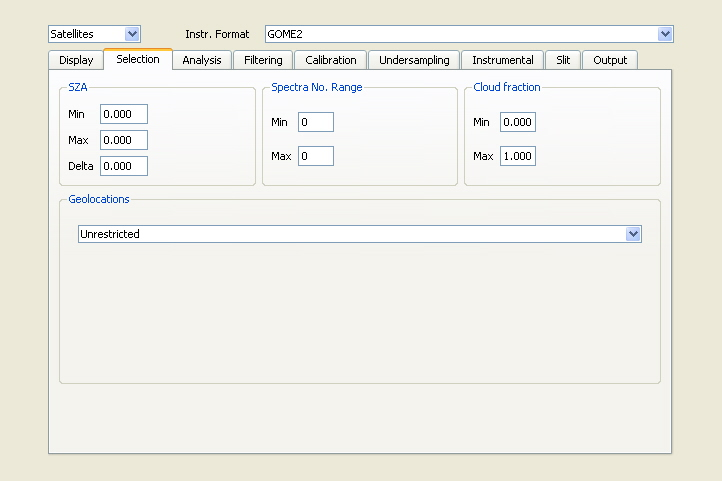
\includegraphics[width=\textwidth]{img/Project_Selection.jpg}
\caption{Projects properties: Selection page}\label{projects_properties_selection}
\end{figure}
\FloatBarrier

\subsubsection{Spectra selection}
This page is dedicated to the selection of spectra to browse or to analyse.  The selection of spectra can be made on:

\begin{longtable}[h]{l p{8cm}}
\textbf{SZA} & specify a range of solar zenith angles and a step in degrees; \\ [6pt]
\textbf{Spectra No} & specify a range of record numbers; \\ [6pt]
\textbf{Cloud fractions} & for satellite measurements, specify a range of cloud fraction (0..1). Until now, only the GOME-2 file format includes information on the cloud fraction. \\ [6pt]
\textbf{Geolocations} & for satellite measurements, selection of pixels based on the geolocation of measurements \\ [6pt]
\end{longtable}

\subsubsection{Geolocation}
Some applications just need satellite overpasses over a list of ground-based stations or above specific regions (satellite validation activities for example).  The geolocation frame gives three possibilities to select pixels over specific locations:

\begin{longtable}{l p{8cm}}
\textbf{Circle} & select pixels within a circle whose the radius is given in kilometers and whose the center could be the position of a station defined by its latitude and longitude; \\ [6pt]
\textbf{Rectangle} & select pixels above a specific region bounded by the limits in longitude and latitude given in degrees (-180..180\degree or 0..360\degree for the longitude according to the satellite file format); \\[6pt]\pagebreak % somehow, latex forgets to put a page break here
\textbf{Sites} & select pixels within multiple circles with radius given in kilometers and center position determined by the longitude and the latitude of the observation sites defined in the \textbf{Sites tab page} (see the \textbf{Output page}, page \pageref{sec:projects_output_page}, for the automatic creation of the output file name).
\end{longtable}

\subsubsection{Elevation angles}
Criteria selection on the elevation angles can be specified for MAXDOAS measurements, for example to select a reference spectrum that is not a zenith or to reject spectra measured at an elevation angle out of the specified interval.

\begin{figure}[!h]
\vspace{+0.8\baselineskip}
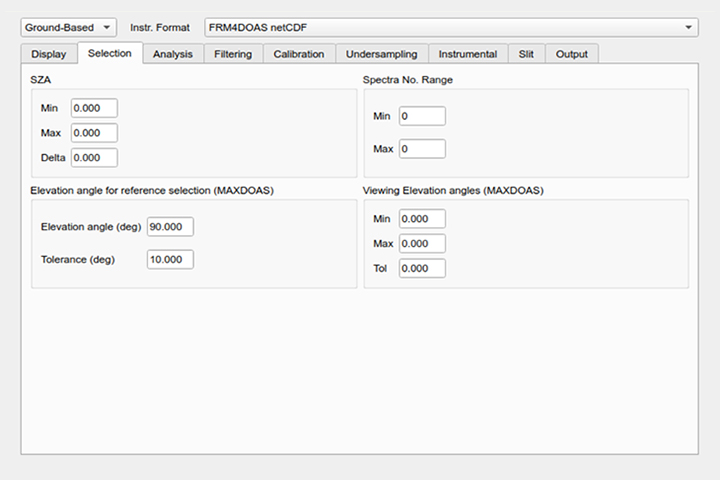
\includegraphics[width=\textwidth]{img/Project_SelectionMaxDOAS.jpg}
\caption{Projects properties: Selection page for MAXDOAS}\label{projects_properties_selection_maxdoas}
\end{figure}
\FloatBarrier

To browse or to analyse all spectra of a file without any constraint, keep default options.

\begin{figure}[!h]
\subsection{Analysis Page} \label{sec:projects_analysis_page} \hfill
\vspace{-0.8\baselineskip}
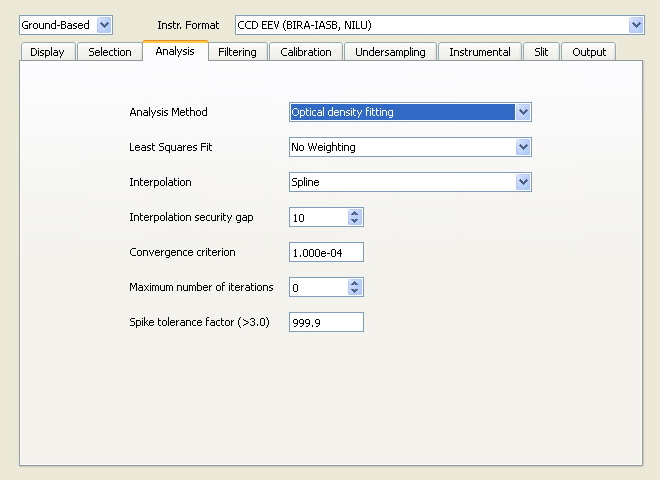
\includegraphics[width=\textwidth]{img/Project_Analysis.jpg}
\caption{Projects properties: Analysis page}\label{projects_properties_analysis}
\end{figure}
\FloatBarrier

Default options of this page are valid for all applications. Expert users can change them to perform some tests. Further details on the retrieval algorithms can be found
in the \textbf{\nameref{cha:descr-algor}} chapter.

\subsubsection{The Analysis Method}
Available retrieval method are:

\begin{itemize} \itemsep -6pt
\item Optical density fitting;
\item Intensity fitting
\end{itemize}

These methods differ by the way the Beer-Lambert equation is expressed and resolved.  Usually the \textbf{Optical density fitting} is preferred to analyze spectra.

\subsubsection{Least-Squares Fit}
The fit can be weighted if instrumental uncertainties on measurements are known.

\subsubsection{Interpolation}
\textbf{Linear} and \textbf{cubic Spline} interpolations are implemented.  \textbf{Spline} interpolation is recommended

\subsubsection{Interpolation Security Gap}
Convolution/filtering/interpolation operations could introduce edge effects if cross sections are strictly defined on the different analysis spectral intervals. In order to avoid that, it is recommended to add some extra pixels on both sides of the final grid. The security gap determines this number of pixels. If the selected filter requires a larger number of additional pixels, the gap is recalculated by QDOAS.

\subsubsection{Convergence Criterion}\label{sec:conv-crit}
As explained in the description of the \nameref{sec:marq-levenb-algor}
in section \ref{sec:doas-retrieval}, the \gls{nlls} algorithm uses the
convergence criterion to determine when it has arrived at a solution.

Usually a value of 1e-3 or 1e-4 is selected for the convergence
criterion.  For higher values of $\epsilon$, the algorithm will use
less iterations, but the accuracy of the results could be affected.

\subsubsection{Maximum Number of Iterations}
The number of iterations needed to analyze a spectrum is determined by the convergence speed of the Marquardt-Levenberg algorithm for this spectrum. For some tests, it is sometimes useful to limit it. A value of ``0'' doesn't limit the number of iterations.

\subsubsection{Spike Tolerance Factor} \label{sec:projects_analysis_spikes}
Spikes removal is a good alternative to the introduction of gaps (see the \textbf{Gaps} section of \textbf{Analysis windows properties}, page \pageref{sec:analysis_gaps_page} to automatically remove bad data points from the fit, such as
satellite measurements affected by the South Atlantic Anomaly or pixels of the detector damaged by electronic radiation.  To do this, QDOAS calculates the \gls{rms} residual after
the fit.  If a pixel $i$ is found where the absolute value of the
residual, $R_i$, exceeds the \gls{rms} by more than the spike
tolerance factor $x$,

\begin{equation}
  \label{eq:spike_removal}
  R_i > x \cdot \mathrm{RMS}\,,
\end{equation}

QDOAS will remove this pixel from the analysis and calculate a new
fit.  This procedure is applied iteratively until no residuals exceed
the \gls{rms} by more than the given tolerance factor.  The analysis results
contain a list of all pixels that were removed.

This feature should be used with caution, as choosing a too low
tolerance factor might exclude valid data points from the fit.
Assuming the residuals are normally distributed with mean 0, the
\gls{rms} can be used as an estimate of the standard deviation
$\sigma$.  As a rule of thumb, the tolerance factor $x$ should be high
enough, so the probability that a normally distributed random variable
lies outside a range of $x\cdot\sigma$ around the mean, multiplied by
the number of pixels in the analysis window, is small.

\begin{figure}[!h]
\subsection{Filtering Page} \label{sec:projects_filtering_page} \hfill
\vspace{-.8\baselineskip}
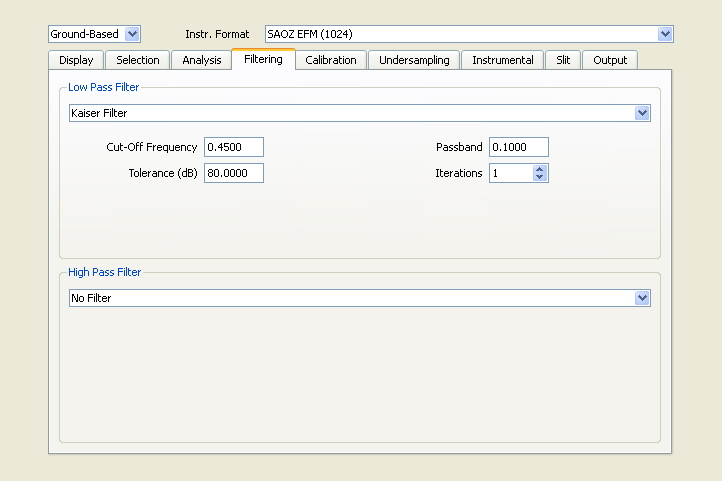
\includegraphics[width=\textwidth]{img/Project_Filtering.jpg}
\caption{Projects properties: Filtering page}\label{projects_properties_filtering}
\end{figure}
\FloatBarrier

Filtering attenuates components in the spectra with frequencies higher (low-pass filtering) or lower (high-pass filtering) than a given cut-off frequency. This simple method can improve the analysis of noisy spectra but may lead in the other hand to a loss of spectral information and should be used very carefully. Filtering corresponds to a convolution in the pixels domain.  The most common filter functions are implemented.  Further details can be found in the literature.

\begin{description}
\item[Kaiser] correction using the algorithm described in \citet{Kaiser_Reed_1977};
\item[Boxcar] convolution with a rectangle function; this filter consists in averaging the spectrum over several spectral points;
\item[Gaussian] convolution with a Gaussian function;
\item[Triangular] convolution with a triangle function;
\item[Savitzky-Golay] this filter uses a least-square linear regression fit of a polynomial of degree $k$ over at least $k+1$ data points around each point in the spectrum;
\item[Binomial] convolution with a filter function formed with the binomial coefficients calculated using the recursive Pascal's triangle algorithm;
\item[Odd-even pixels] smoothing obtained by averaging spectra interpolated on odd and even pixels.
\end{description}

According to the selected filter, different fields have to be completed.
Select filter type \textbf{No Filter} if you want to disable spectra and cross sections filtering.

Filtering is applied after interpolation of the original spectra or cross sections on the final grid.

\subsubsection{Low-Pass Filtering}
Low-pass filtering is applied to the spectra and to the cross sections. Nevertheless, the filtering of cross sections could be disabled individually in the \textbf{Analysis windows properties} dialog box.

\subsubsection{High-Pass Filtering}
Cross sections are filtered by subtracting (optical density fitting) or dividing (intensity fitting) a fitted polynomial or a smooth spectrum calculated by filtering the original cross sections a high number of times. This can be an alternative to the Gram-Schmidt algorithm to calculate differential cross sections.

For the moment, high-pass filtering is supported only in optical density fitting mode. It can be applied during the phase of calibration and/or during the analysis of spectra.

\subsection{Calibration Page}\label{sec:projects_calibration_page}
The configurtion of the wavelength calibration procedure is explained in detail in section \ref{sec:conf-wavel-calibr}.

\begin{figure}[!h]
\subsection{Undersampling Page} \label{sec:projects_undersampling_page} \hfill
\vspace{-.8\baselineskip}
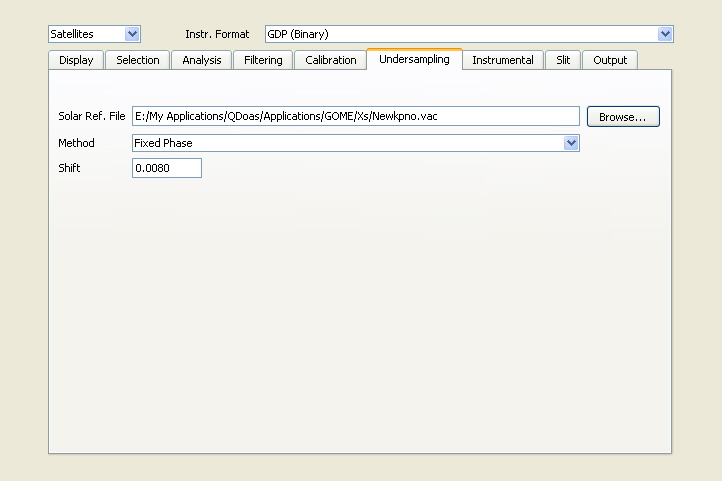
\includegraphics[width=\textwidth]{img/Project_Undersampling.jpg}
\caption{Projects properties: Undersampling page}\label{projects_properties_undersampling}
\end{figure}
\FloatBarrier

The undersampling is a well-known problem of GOME onboard the
satellite ERS-2. It arises from the poor sampling ratio of the GOME
instrument (2 to 3 pixels/\gls{fwhm} of the resolution of the
spectrometer) which results in a lost of spectral information when
interpolating earthshine spectra during the DOAS fitting process. The
problem can be corrected using ad-hoc cross sections obtained by
simulating the effect from a high-resolution solar
reference. Undersampling cross sections can be pre-calculated using
the \textbf{\nameref{sec:tool_undersampling}} or they can be
calculated in real time, just after the wavelength calibration
procedure using the corrected grid and the determined slit function.

To apply undersampling correction, the fit button of \textbf{Usamp 1} and/or \mbox{\textbf{Usamp 2}} items in the \textbf{Predefined parameters} page of \textbf{Analysis windows properties} (cfr page \pageref{sec:undersampling_params}) has to be checked in addition of the selection of options of this page.
By default, no undersampling correction is applied.

\subsubsection{Method}
Different methods for the calculation of the undersampling correction are available.
\begin{longtable}[h]{l p{8cm}}
\textbf{From file} & Undersampling cross sections are provided in files like usual cross sections. These files might be created using the \textbf{\nameref{sec:tool_undersampling}}. The files have to be provided in the \textbf{Analysis windows properties} (\textbf{Molecules} or \textbf{Predefined paremeters} page according to the selected analysis method). \\ [6pt]
\textbf{Fixed phase} & QDOAS uses the information derived from the calibration procedure to create the undersampling cross sections, with a fixed value of the shift. The selection of this method is recommended. \\ [6pt]
\textbf{Automatic phase} & The undersampling cross sections are calculated at each iteration of the analysis procedure, using the fitted value for the shift between the reference and the measured spectra. This method is rather time consuming and only applicable for testing purposes.	 \\ [6pt]
\end{longtable}

\subsubsection{Solar ref. file}
In \textbf{Fixed phase} and \textbf{Automatic phase}, undersampling cross sections are calculated from a high resolution solar spectrum convolved on an oversampled and an undersampled grid with the instrument slit function (according to \textbf{calibration options}, the slit function characterized by the calibration procedure or a slit function provided by the user in the \textbf{slit page} of \textbf{Projects properties}).

\subsubsection{Shift}
The \textbf{Shift} field operates only in \textbf{Fixed phase} method.

\begin{figure}[!ht]
\subsection{Instrumental Page} \label{sec:projects_instrumental_page} \hfill
\vspace{-.8\baselineskip}
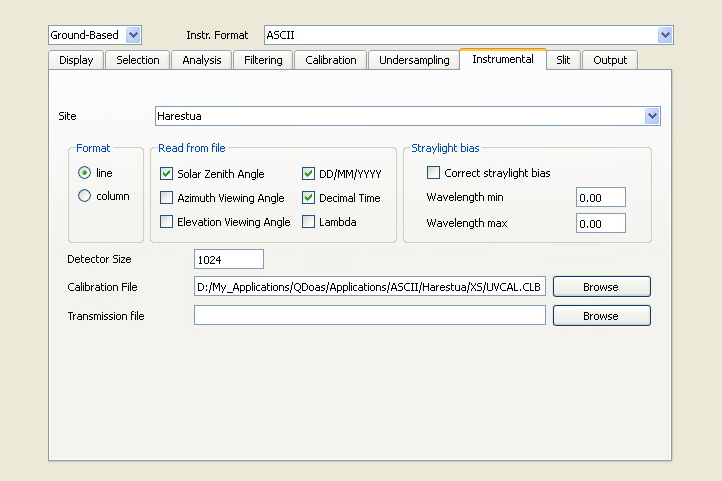
\includegraphics[width=\textwidth]{img/Project_InstrumentalAscii.jpg}
\caption{Projects properties: Instrumental page}\label{projects_properties_instrumental}
\end{figure}
\FloatBarrier

The fields that appear in this page strictly depend on the format of spectra files to process.

\subsubsection{Ground-based measurements}The size of the detector is the first information to provide in this page.  Except if a preliminary wavelength calibration is provided with the spectra, a wavelength calibration file is necessary to browse spectra.
For ground-based measurements, the observation site allows (re)calculating solar angles.  The calculated solar azimuth angles will follow the provided SAA convention.

\textbf{Important note} : Even if the native MFC binary and standard formats generated by DOASIS and MS-DOAS acquisition S/W can still be selected, no further development and support is provided.

\subsubsection{Calibration File And Instrumental Corrections}

\textbf{For the analysis of spectra, the wavelength calibration of the reference spectrum always has the priority over the spectra ones.  It is important to select this file very carefully mainly when browsing spectra to save a new reference spectrum.}

Some instrumental corrections can be applied on spectra. For example, a transmission function previously determined in laboratory with calibrated sources can be specified in the \textbf{Transmission file} field. A two columns ASCII file is expected (wavelength calibration and transmission function) and spectra will be divided by this curve before the wavelength calibration procedure.

Dark current correction is also possible according to the file format. The selected file format determines how dark currents are provided and how spectra are corrected.  See below for \textbf{Dark Current And Offset Correction for the MFC format (original binary and std formats generated by DOASIS or the one specific at BIRA-IASB}.

For satellite measurements, the wavelength calibration of earthshine spectra and irradiances is provided in the files and no transmission file is needed. Both fields should then be kept empty. The only information to provide should be the spectral region to process: the band type (for GOME and GOME2) or the channel and the clusters (for SCIAMACHY).

\subsubsection{Dark Current And Offset Correction For The MFC Format}
According to the file format, measured dark current are available and
subtracted from spectra just before the analysis.  Since version
2.111, QDOAS supports both MFC binary and STD ASCII formats generated
by the well-known DOASIS program created by the atmospheric research
group at IUP Heidelberg, Germany and widely used in the DOAS community.

\begin{center}
\href{https://doasis.iup.uni-heidelberg.de/bugtracker/projects/doasis/}{https://doasis.iup.uni-heidelberg.de/bugtracker/projects/doasis/}
\end{center}

In addition, BIRA-IASB has developed its own binary MFC format in which all spectra including dark currents and offsets of a same day are saved in a unique file.  A MFC STD to MFC BIRA-IASB binary format converter exists (see the \textbf{MFC Binary section}, page \pageref{sec:MFC_bin}).

For the BIRA-IASB binary format, dark currents and offsets present in a file are averaged before spectra correction.  For the MFC binary and std formats generated by DOASIS, dark current and offset are provided in two separate files in the original format.  Dark currents should be spectra measured with a large integration time (typically 30 sec) and offsets should be the average of a large number of spectra measured with a very small integration time (typically 1000 x 3 ms).

Application of the offset correction:
\begin{equation}
\mathrm{spe}^\prime=\mathrm{spe}-\mathrm{offset}\cdot(\mathrm{scans}_\mathrm{spe}/\mathrm{scans}_\mathrm{offset})\, ,
\end{equation}
\begin{equation}
\mathrm{drk}^\prime=\mathrm{drk}-\mathrm{offset}\cdot(\mathrm{scans}_\mathrm{drk}/\mathrm{scans}_\mathrm{offset})\, ,
\end{equation}
where $\mathrm{scans}_\mathrm{spe}$, $\mathrm{scans}_\mathrm{drk}$ and $\mathrm{scans}_\mathrm{offset}$ are respectively the number of scans for the spectrum, the dark current and the offset.

Correction of spectra with the dark current (previously corrected by offset):
\begin{equation}
\mathrm{spe}^\prime=\mathrm{spe} - \mathrm{drk}\cdot (\mathrm{et}_\mathrm{spe}\cdot\mathrm{scans}_\mathrm{spe}) /(\mathrm{et}_\mathrm{drk}\cdot\mathrm{scans}_\mathrm{drk})\, ,
\end{equation}
where $\mathrm{et}_\mathrm{spe}$ and $\mathrm{et}_\mathrm{drk}$ are respectively the exposure time of the spectrum and the dark current and $\mathrm{scans}_\mathrm{drk}$ is the number of scans of the dark current.

\subsubsection{The Observation Site}
The information on the observation \textbf{Site} is used to (re)calculate solar zenith angle from geolocation coordinates given for this site in the \textbf{Sites} sheet. This can be useful for example if the solar zenith angles saved in the files are not reliable enough. The abbreviation of the observation site is also used to automatically generate output file names (see the \textbf{Output Page}, page \pageref{sec:projects_output_page}).  The longitude is particularly useful to select reference spectra of the day using the local time instead of Universal Time in case fractional days and times given in UT are distributed in two days (for example, measurements in China).

\subsubsection{Straylight bias}
Requested for some spectra files format, this option allows subtracting from a spectrum the signal averaged on the specified range of wavelengths.
This is useful for example, to retrieve \SO2 in the UV region where the signal is very poor and where the straylight is problematic.  Even if the straylight can be attenuated by subtracting from the spectra, the average of the signal measured in the UV region (below 300 nm if possible), it is recommended to characterize it in laboratory.

\subsubsection{OMI Options}
QDOAS provides some specific options to handle OMI files.  To make
optimal use of these options, refer to the detailed description of the
OMI L1B data in the \citet{OMI_iods}.
\begin{figure}[!ht]
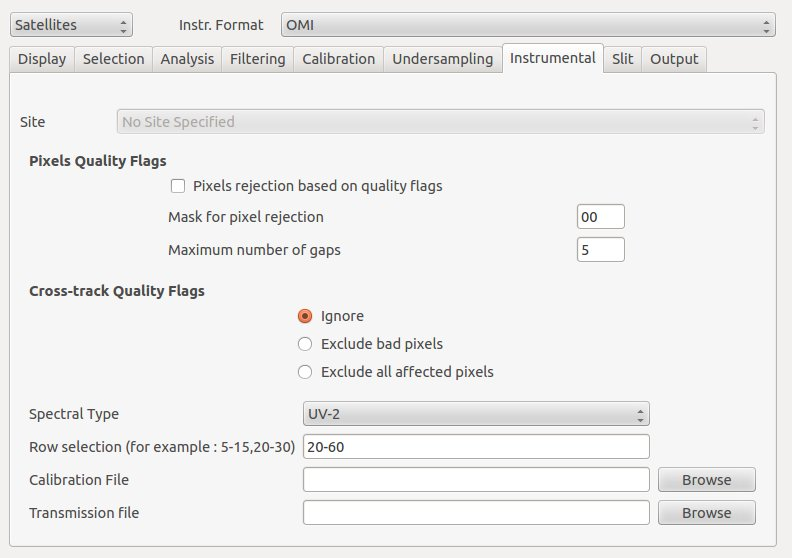
\includegraphics[width=\textwidth]{img/Project_Instrumental_OMI.jpg}
\caption{Projects properties: Instrumental page for OMI.}\label{img:project_instrumental_omi}
\end{figure}

\begin{description}
\item[Pixel Quality Flags] These flags indicate if a wavelength pixel
  was affected by measurement problems such as dark current, stray
  light or saturation.  Using this setting, QDOAS can exclude single
  pixels from the fitting procedure if certain flags are set.

  To use the flags, check ``Pixel rejection based on quality flags''.

  The field ``Mask for pixel rejection'' should contain a hexadecimal
  number indicating which flags should lead to rejection.  For
  example, to exclude pixels with flags 0, 1 and 3 set, one would
  choose a mask
  \begin{equation*}
    2^0 + 2^1 + 2^3 = 11 = \mathrm{B}_{16}\,.
  \end{equation*}
  to reject all flags, one would choose the mask
  \begin{equation*}
    2^0 + 2^1 + \ldots + 2^{15} = 65535 = \mathrm{FFFF}_{16}
    \,.
  \end{equation*}
  For a full description of the 16 PixelQualityFlags in the OMI L1B data,
  refer to the \citet{OMI_iods}.

  The value ``Maximum number of gaps'' indicates the maximum number of
  pixels that should be excluded from the spectrum.
\item[Cross-track Quality Flags] Cross-track Quality Flags describe
  the so-called ``row anomaly'' affecting the OMI data.  These flags
  apply to a complete spectrum and indicate how badly the spectrum is
  affected.  QDOAS provides three options for the handling of these
  flags (see \citep{OMI_iods}):
  \begin{description}
    \item[Ignore] Use all spectra, disregarding the quality flags.
    \item[Exclude bad pixels] Only exclude rows flagged as 'Affected,
      Not corrected, do not use' in the L1B data.
    \item[Exclude all affected pixels] Only use rows flagged as 'Not
      affected'.
  \end{description}
\item[Spectral Type] OMI measurements contain data from three spectral
  bands: UV-1, UV-2 and VIS.
\item[Row selection] This option allows the user to select a subset of
  the 60 detector rows for the analysis, by providing a list of ranges
  from 1 to 60.
\end{description}

\begin{figure}[!h]
\subsection{Slit Page} \label{sec:projects_slit_page} \hfill
\vspace{-.8\baselineskip}
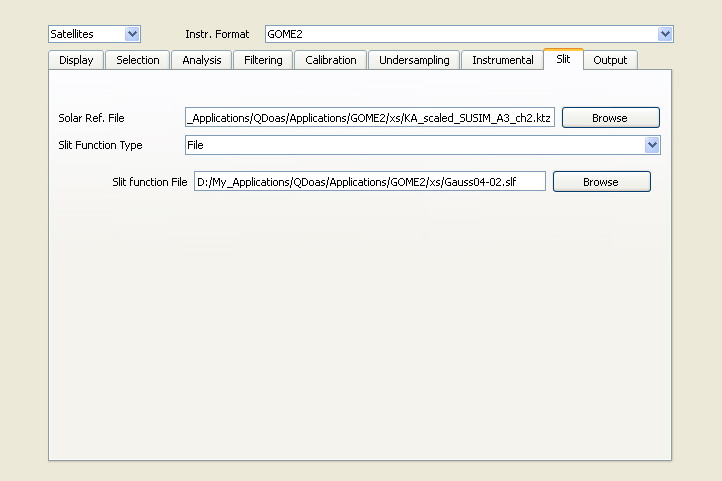
\includegraphics[width=\textwidth]{img/Project_Slit.jpg}
\caption{Projects properties: Slit page}\label{projects_properties_slit}
\end{figure}
\FloatBarrier

Input cross sections have to be degraded to the resolution of the instrument before the analysis. This can be done using the \textbf{convolution tool}. However the programme also authorizes the direct use of high-resolution cross sections which will be convolved in real time using information provided in this page \underline{\textbf{if and only if}} the slit function is not characterized by the \textbf{wavelength calibration procedure}.

\subsubsection{Slit Function Type}
Several analytic line shapes are proposed including line shapes supported by the \textbf{wavelength calibration procedure} (gaussian, lorentzian, error function, voigt and asymmetric line shapes). Different fields have to be completed according to the selected slit function. ASCII file is requested for slit functions measured in laboratory (option \textbf{File}) or when the ``Wavelength dependent'' button is checked (analytical line shapes).

\begin{itemize}
\item \underline{Slit functions measured in laboratory}: the first column should be the wavelength grid of the line shape; the maximum of the line shape is expected around 0 nm;  look-up tables can be specified for line shapes defined at different wavelengths (in this case, the first line gives the individual wavelengths).
\item \underline{Wavelength dependent analytical slit functions}: the input file should contain the \gls{fwhm} variation with the wavelenth calibration; at a given wavelength, cross sections will be convolved with the appropriate resolution.
\item \underline{Wavelength dependent stretch factors on a user-defined slit function}:
To account for an asymmetry of the slit function that varies with the wavelength, a three columns ASCII file can be specified in addition to the slit function file.  This ``Stretch on wavelength'' file should contain the wavelength calibration and the two values of the stretch to apply on the grid of the line shape, one for each side of the slit function.
Such a file can be obtained by merging in one file the parameters SFP1 and SFP2 resulting of the wavelength calibration (use the \textbf{Save As} option from the title of the plots to save the curves in an ASCII file).
\end{itemize}

\subsubsection{Solar Reference File}
A high-resolution solar spectrum is expected to replace the solar spectrum of the \textbf{Calibration page} if the slit function is not characterized during the calibration procedure and solar spectrum and cross sections have to be convolved with the line shape specified in this page.
Otherwise, if the slit function type of this page is \textbf{None}, preconvolved solar spectrum (in this page) and cross sections (in \textbf{Analysis windows properties}) are expected.

\begin{figure}[!h]
\subsection{Output Page} \label{sec:projects_output_page} \hfill
\vspace{-.8\baselineskip}
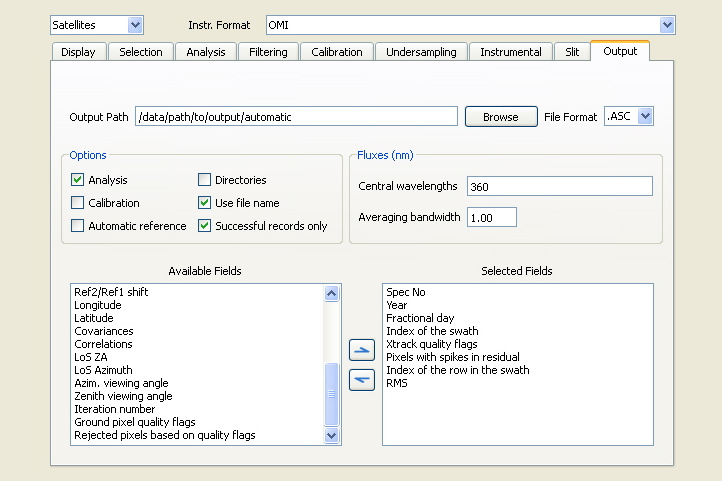
\includegraphics[width=\textwidth]{img/Project_Output.jpg}
\caption{Projects properties: Output page}\label{projects_properties_output}
\end{figure}
\FloatBarrier

This page is dedicated to the selection of information on analyzed records to write in the output file after calibration and/or analysis of spectra. When the \textbf{Analysis button} is checked, all the fields in this page are enabled and it is also possible to select the fit results that should be saved in the \textbf{Analysis windows properties} pages.

When the user selects chooses ``.ASC'' as the file format, the program produces ASCII files with tab-separated columns for all selected output fields.  These files may be loaded in spreadsheets such as Excel.  The first line of the analysis output starts with a hash (\#) character and is used to print the column titles.  When the \textbf{Calibration button} is checked, wavelength calibration results are saved before the analysis results. Lines with calibration output start with a semicolon (;).  \textbf{If an ASCII output file already exists at the specified location, QDOAS appends the new results to the existing file.}  In this case, column titles and calibration information are not repeated.  Therefore, it is best to avoid writing to existing files, unless exactly the same analysis and output configuration is used to produce the new data.  \textbf{To replace the content of an existing output file, the file must first be deleted manually}.

With the file format ``.nc'', QDOAS will produce netCDF output data.
This is the recommended setting for users who wish to use a binary
output format.  In contrast to ASCII mode, results from different
processing runs cannot be appended to the same file in netCDF mode,
unless the user chooses a different group name for both runs (the
default group name is the project name).  When using QDOAS with a
single output file, the program will check if a netCDF file with that
filename already exists, and report an error if the file already contains a group with the chosen group name.  However, when writing files in ``automatic'' mode
(see \nameref{sec:autom-creat-outp}), QDOAS doesn't check in advance
which output file(-s) it will have to write, and it is left to the
user to make sure that there are no existing files in the output path
which will prevent QDOAS from saving the results of a processing run.

QDOAS always saves all the output from a single input file in one shot, either when it has processed the last spectrum of an input file, or when the analysis is stopped using the \textbf{stop button} 
\includegraphics[width=3mm]{img/Button_Stop.png}.

By default, QDOAS only saves records successfully analyzed.  If the button \textbf{Successful records only} is kept unchecked, all records including reference spectra and records for which the analysis fails (e.g. log error on the spectrum) are saved.

When processing was unsuccessful, QDOAS uses the fill value
9.969\ldots e+36 for floating point output data, an empty string for
text output fields, and values -32767, 65535 or -2147483647 for
integer output fields, depending on the range of the output field.
For the netCDF output format, fill values are written to the
\_FillValue attribute of the corresponding variables.

\subsubsection{Automatic Creation Of The Output File Name}\label{sec:autom-creat-outp}
The path and the name of the output file can be specified in the \textbf{Output Path} field.  If ``automatic'' is used as a file name, QDOAS will generate the name of the output file automatically, using the user-defined output path as a base.

For ground-based measurements, the \textbf{Directories} and \textbf{Automatic reference} buttons have no effect. The original file name is always used (but the file extension is changed in \textbf{``.asc''}) except if the \textbf{Use file name} button is unchecked and an observation site has been specified in the \textbf{Instrumental page}. In this case, the output file name is built as follows:
\begin{center}
$<$output path$>$/XXYYYYMM.ASC
\end{center}
Where:

\begin{longtable}[h]{l p{8cm}}
\textbf{output path} & is the user-defined path; \\ [6pt]
\textbf{XX} & is the abbreviation of the observation site selected in the \textbf{Instrumental} tab page; if no observation site is specified, the original file name is used; \\ [6pt]
\textbf{YYYY} & is the year of measurement; \\ [6pt]
\textbf{MM} & is the month (zeros padded) of measurement; \\ [6pt]
\textbf{ASC} & is the default file extension for ASCII files;	\\ [6pt]
\end{longtable}

For satellite measurements, the \textbf{Use file name} button has no effect. If overpasses calculation is requested (option \textbf{Sites} in the \textbf{Geolocation} frame of the \textbf{Selection} page), then the output file name is determined as above ($<$output path$>$/XXYYYYMM.ASC where XX is the abbreviation of the station). Otherwise, for SCIAMACHY files, the output file name automatically created has the syntax SCIA\_YYYYMMDD\_NNNN.ASC where YYYYMMDD is the date of measurement (year, month, day) and NNNN the orbit number. For other satellite formats, the original file name is used (but with the file extension \textbf{``.ASC''}). Files are distributed in a year/month/day folder structure if the \textbf{Directories} button is checked.

\subsubsection{Fluxes}
The \textbf{flux} is the value of the signal averaged over pixels within a bandwith around the specified wavelength.  Divided by the exposure time, this can be used to check a relative intensity.  To calculate and save fluxes in the output file, specify the central wavelengths separated by the semicolon (;) character. For example, to get fluxes at 330 nm, 350 nm and 380 nm, enter:
\begin{center}
330; 350; 380;
\end{center}
The averaging bandwidth in nm is also requested (for example a bandwidth of 1 nm means that pixels within the central wavelength +/- 0.5 nm will be averaged).
Coulour indexes are the ratio between two fluxes and can be easily recalculate from output fluxes.

\subsubsection{Selection Of Fields To Output}
The content of this frame is similar to the one in the \textbf{Display page}.  In QDOAS, the output is fully configurable. Information related to the measurements (e.g. date and time, viewing angles, geolocation coordinates,~\dots) can be selected in this page. The selection of analysis results (e.g. slant column densities, fitted non-linear parameters,~\dots) is made individually in the \textbf{Analysis windows properties} pages. The selected instrument or file format determines the list of fields available for output. For example, information on cloud fraction and cloud top pressure is available only for satellite instruments. A non-exhaustive list of fields available for ground-based and satellite measurements is given in appendix \textbf{\ref{cha:output}}.

\begin{figure}[!h]
\section{Analysis windows properties}
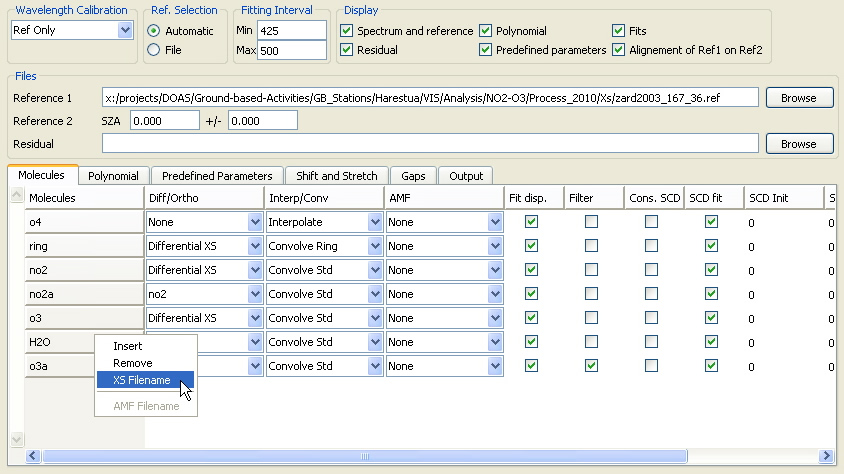
\includegraphics[width=\textwidth]{img/Analysis_Properties.jpg}
\caption{Analysis windows properties}\label{analysis_properties}
\end{figure}
\FloatBarrier

This dialog box completes the \underline{\textbf{Projects properties}} for the configuration of the analysis of spectra. Several analysis windows can be defined under a same project.  Next section will guide you in the definition of parameters to fit.

\subsubsection{Fitting interval}
The fitting interval is the first option to specify when a new analysis window is created. It depends on the region covered by the spectrometer and the trace gases to retrieve. According to the molecules to focus on, some baseline recommendations can be found in the literature.

\subsubsection{Reference Spectra}
In the DOAS technique, spectra are always analyzed with respect to a reference spectrum. This could be the irradiance spectrum of the current satellite file, any other reference spectrum provided in an ASCII file or a daily reference spectrum selected on a solar zenith angle criterion. The \textbf{Ref. Selection} box proposes to choose between the modes \textbf{File} (irradiance of the file for satellites measurements or an external reference spectrum) and \textbf{Automatic} (reference spectrum selected on specific criteria).

In addition, QDOAS gives the possibility to define two reference spectra (\textbf{Reference 1} and \textbf{Reference 2}). \textbf{Reference 1} is always a file; according to the \textbf{Ref. Selection mode}, \textbf{Reference 2} can be the name of an ASCII file or a spectrum automatically selected by the program. These options determines on which reference spectrum the wavelength calibration procedure is applied:
\begin{itemize}
\item If only one reference spectrum is specified (\textbf{Reference 1} or \textbf{Reference 2}), it is used as control spectrum i.e. the \I0 spectrum in the Beer-Lambert law. The wavelength calibration procedure is applied on this spectrum and the cross sections are re-interpolated on the new calculated grid before the analysis of spectra.
\item If two reference spectra are given, the wavelength calibration is applied only on the first one (\textbf{Reference 1}); the shift between both reference spectra is then determined (using a \gls{nlls} fitting approach) in order to align cross sections on the second reference spectrum (\textbf{Reference 2}) and spectra are analysed w.r.t. \textbf{Reference 2}.
\end{itemize}

\subsubsection{Automatic Reference Selection}
The information on the \gls{sza} is present in most ground-based file formats.  According to the SZA range, a reference spectrum with the SZA the closest to the given value is selected for each twilight or the spectrum with the minimum SZA of the day is selected (both values initialized to 0 or the SZA range below all SZA values of the file).

For \textbf{MAXDOAS measurements}, it is also possible to select the zenith spectrum of the scan.  Currently, \textbf{Scans/SZA} radio buttons appear to make this selection possible with the BIRA-IASB CCD EEV format, MFC binary and std formats generated by DOASIS, MFC BIRA binary format and ASCII format.  If this option is necessary for other file formats, please, contact \href{mailto:caroline.fayt@aeronomie.be}{authors}.

\begin{figure}[!h]
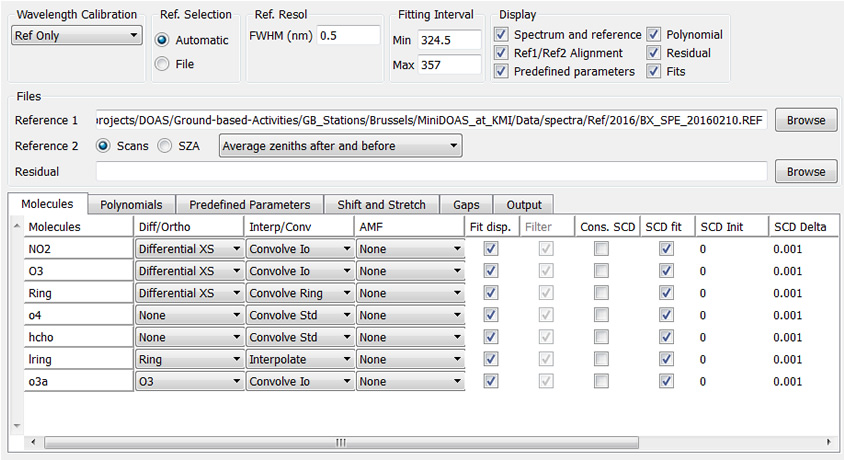
\includegraphics[width=\textwidth]{img/Analysis_Properties_Scans.jpg}
\caption{Automatic reference selection in scan mode for MAXDOAS measurements}\label{analysis_properties_scans}
\end{figure}
\FloatBarrier

Currently, in mode ``reference of the scan'', four options are available :

\begin{itemize} \itemsep -3pt
\item select the last zenith before the current scan;
\item select the first zenith after the current scan;
\item average the zenith spectra before and after the scan;
\item interpolate at the current measurement time, the zenith spectra before and after the scan.
\end{itemize}

Note that if one of the two zenith spectra (the zenith just before or after the current scan) is missing, the other one is automatically used as reference.

For \textbf{satellite measurements}, if no \textbf{Reference 1} is specified (field kept empty), the irradiance of the current file is always implicitly used. This means that if a \textbf{Reference 2} is provided, the wavelength calibration is applied on the irradiance spectrum (\textbf{Reference 1}) of the file and the control spectrum (\textbf{Reference 2}) will be aligned on the irradiance before the analysis of earthshine spectra.  For satellite measurements, the \textbf{Reference 2} spectrum could be an average of spectra selected in a specific region given by its minimum and maximum latitudes and longitudes. Other information such as the cloud fraction (GOME2) could also be used to refine the reference selection.
% TODO detailed info on automatic reference selection procedure for OMI/GOME2/other satellite instruments?

\subsubsection{Wavelength Calibration}
The quality of the fit results largely relies on a very accurate determination of the wavelength calibration of the reference spectrum.  The wavelength calibration procedure developed in QDOAS allows correcting the preliminary grid of the reference spectrum using a high-resolution solar atlas spectrum degraded to the resolution of the instrument (see the \textbf{Calibration page}, page \pageref{sec:projects_calibration_page} of \textbf{Projects properties}).  The information on the shift and eventually the slit function retrieved from this procedure are used to convolve/interpolate the cross sections before the analysis.  The wavelength calibration is always applied in priority on the \textbf{Reference 1} (the irradiance spectrum for satellite measurements). If two reference spectra are provided, \textbf{Reference 2} is aligned on \textbf{Reference 1} using the same non linear least-square algorithm as the one used for the analysis of spectra w.r.t. the control spectrum.

If the wavelength calibration of the reference spectrum is assumed to be accurate enough, the option \textbf{None} can be used instead of \textbf{Ref Only}. The option \textbf{Spectra only} is useful for some particular applications (for example, long paths measurements for which the reference spectrum is a lamp measurement).

The option \textbf{Ref+spectra} allows applying a calibration correction on both reference spectrum and spectra to analyze. This option has been designed to handle spectra recorded with unstable (unthermostated) instruments where the spectral resolution can vary a lot from one spectrum to another. In this case, the resolutions of both spectra are matched to the resolution of the less resolved spectrum, and the absorption cross sections can be convolved in real-time to the same effective resolution. This option is time consuming and should be used carefully.

\subsubsection{Display}
After the processing of a spectrum, QDOAS can plot for each spectral analysis window:
\begin{itemize} \itemsep -3pt
\item the spectrum and the reference in the fitting interval;
\item the residual of the fit (the difference between the observed and the calculated);
\item the continuum part of the spectrum fitted by a polynomial;
\item the fit obtained for each species
\item the predefined parameters (offset, undersampling);
\item in the case two reference spectra have been selected, these two spectra after the alignment correction.
\end{itemize}
The appropriate buttons are checked according to the graphs to plot.  An individual selection of the cross sections and the predefined parameters can still be performed in the dedicated tab pages.

\subsubsection{Residuals}
If a file is specified in the \textbf{``Residual''} filename field,
Qdoas will use this file to output the fitting residuals.  This
feature can be used in order to study the residuals, or, when
systematic residual structures structures are identified, in order to
create a synthetic cross section that could be introduced in the fit.
Because Qdoas appends the residuals of each analysis run to the end of
the file, the size of the file can increase rapidly and it is
recommended to disable this option by emptying the
\textbf{``Residual''} file name field when it is no longer needed.

The residual file contains one line for each processed record.  The
first three numbers are the record number, the solar zenith angle and
the decimal time respectively.  Then, the residuals for each wavelength
of the original spectrum are given.  For wavelengths which are not
part of the chosen analysis window, or which were removed by the spike
removal algorithm, a ``nan'' value is written.  The first line of the
file contains the calibrated wavelength for each column, preceded by
the three numbers \texttt{0 0 0}.  An example:

\begin{Verbatim}[fontfamily=courier,fontsize=\relsize{-2}]
0 0 0 4.25848e+002 4.25689e+002...  4.99708e+002 5.00065e+002
16 81.024 7.2989 nan ... nan -3.992e-004 ...  -6.663e-005 2.460e-004 nan ... nan
17 80.668 7.3006 nan ... nan 3.584e-004 ...  1.611e-004 9.982e-004 nan ... nan
18 80.396 7.3019 nan ... nan 2.594e-004 ...  7.704e-005 9.206e-004 nan ... nan
\end{Verbatim}

\subsubsection{Fitting Parameters}
The user must define the fitting parameters in the appropriate pages of the property sheet at the bottom of the dialog box. The different pages are:

\begin{description}
\item[Molecules] definition and configuration of the list of cross sections to fit;
\item[Polynomials] specification of the degree of the polynomial used to fit the continuous component of the absorbance, and the polynomial used for linear offset fitting;
\item[Predefined Parameters] this page proposes several predefined parameters such as offset, undersampling, \dots  ;
\item[Shift and Stretch] shift and stretch can be applied to any spectral item;
\item[Gaps] gaps can be introduced in the fitting window (e.g. to eliminate bad pixels)
\item[Output] selection of the calculated column densities and associated errors that should saved in the output file.
\end{description}

According to the associated type of parameters, the selected page proposes several columns of options to fill in, to check or to select from a multiple choice. The conviviality of the analysis parameterisation is enhanced by the use of right-click shortcut menus to handle the lists of items in the different tab pages.  Because of the complexity of the whole set of options, the structure is detailed page after page in the following section.

\section{Configuration of the fitting parameters} \label{sec:analysis_config_param}
\subsection{The Molecules Page}
This page contains options for defining and configuring the list of cross sections to fit (see figures below):

\begin{figure}[!h]
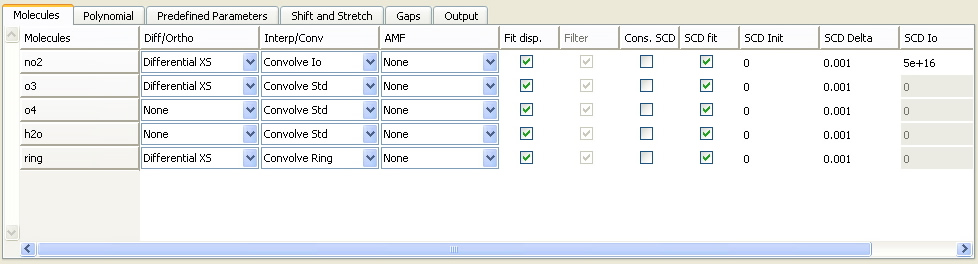
\includegraphics[width=\textwidth]{img/Analysis_Molecules.jpg}
\caption{Analysis Windows Properties: Molecules Page}\label{analysis_molecules}
\end{figure}
\FloatBarrier

Molecules are characterized by their cross section. They are represented by symbols previously defined in the \textbf{Symbols} page of the user interface. QDOAS needs these symbols for internal use: to create lists of available molecules for specific options (for example: in the \textbf{Differential cross sections} column or in the \textbf{Shift and stretch} page) and to build cross section files filters.
\begin{itemize}
\item \textbf{For internal needs of the program, cross section files names must imperatively start with the symbol name as prefix followed by the underscore character !}
\item There is no constraint on the cross section file extension; the default one used by QDOAS for creating cross sections files filters starts with ``xs''.
\end{itemize}
Right-click and select \textbf{Insert}, \textbf{Remove} or \textbf{XS Filename} options in the contextual menu respectively to insert a new molecule in the list, to delete an existing one or to modify the file associated to a cross section. The \textbf{Remove} option is disabled for a symbol if another cross section is orthogonalised to the selected one or if the selected symbol is used in the \textbf{Shift and Stretch} pages.

\subsubsection{Differential cross sections} \label{differential_xs}
Differential cross sections can be generated by orthogonalisation or high-pass filtering according to the definition of an orthogonal base formed with the component vectors (generally, a base of order 2) of the polynomial defined in the \textbf{Polynomial} page. Refer to the \textbf{\nameref{cha:descr-algor}} chapter for further details.  Three options are available:

\begin{description}
\item[None] the original cross section is used;
\item[Differential XS] a differential cross section is generated, either
  \begin{enumerate}
  \item by orthogonalisation if an orthogonal base is defined in the \textbf{Polynomial} page (Gram-Schmitt algorithm);
  \item using high-pass filtering options defined in the \textbf{Filter} tab page of \textbf{Projects properties} otherwise.
  \end{enumerate}
\item[Cross section] When choosing another cross section from the
  proposed list, the selected cross section is orthogonalised to the
  orthogonal base (if defined) and to the cross section chosen from
  the list (orthogonalisation in cascade is allowed).
\end{description}

The latter case prevents from possible correlation between two cross sections (for example, two \ozone~cross sections measured at different temperatures typically to separate contributions from the stratosphere and the troposphere or cross sections with strongly correlated absorption structures, eg. \BrO~and \H2CO). The list of available cross sections includes all cross section symbols defined in this page except the one selected. It is updated as cross sections symbols are added to or removed from this page.

\subsubsection{Interpolation/Convolution}
Cross sections should be defined on the grid of the control spectrum before the analysis. This column describes the action to perform on the selected cross section:

\begin{longtable}[h]{l p{8cm}}
\textbf{None} & the selected cross section is assumed to be correctly aligned on the reference spectrum grid; so, no action will be performed on the cross section (for example, a user-defined undersampling cross section in optical density fitting); \\ [6pt]
\textbf{Interpolate} & the selected cross section will be interpolated on the grid of the reference spectrum; a cross section already pre-convolved at the resolution of the instrument is expected in input. \\ [6pt]
\textbf{Convolve Std} & this option gives the possibility to convolve a high-resoluted cross section in real-time using either the information on the calibration and the slit function provided by the \textbf{wavelength calibration procedure} or the user-defined slit function specified in the \textbf{Slit Function page} of \textbf{Projects properties}. If the wavelength calibration procedure is applied on both the control spectrum and spectra to analyse, the cross section is convolved with the poorest resolution; \\ [6pt]
\textbf{Convolve \I0} & the cross section is convolved with \I0 correction using the concentration defined in the column \textbf{$SCD$ \I0} (this is the slant column density of the cross section used to calculate the theoretical optical depth in convolution with \I0 correction (see \citet{aliwell_2002}); \\ [6pt]
\textbf{Convolve Ring} &	in the same way, the program can generate a Ring cross section; the expected input file must be a Ring cross section pre-calculated by the \textbf{QDOAS Ring tool} on a high-resoluted grid;  \\ [6pt]
\end{longtable}

Convolving cross sections in real time is a comfortable option that avoid the pre-convolution of all cross sections with respect to the selected reference spectrum and the calibration options.

\subsubsection{AMF}
Usually, it is better to calculate vertical columns outside of QDOAS using an appropriate radiative transfer model (e.g. \glslink{lidort}{LIDORT}, \glslink{disort}{DISORT}). Nevertheless, QDOAS gives the possibility to calculate vertical columns or to correct a cross section using pre-calculated \gls{amf} through options proposed in the \textbf{AMF} column:
\vskip 6pt
\begin{longtable}[h]{p{2.5cm} p{9.cm}}
\textbf{SZA} & vertical columns are calculated using AMF depending only on the solar zenith angle; \\ [6pt]
\textbf{Climatology} & vertical columns are calculated using climatological air mass factors; the AMF depends on the solar zenith angle and the calendar day; \\ [6pt]
\textbf{Wavelength} & before the analysis, the selected cross section is corrected using wavelength dependent AMF (modified DOAS). \\ [6pt]
\end{longtable}

Additional option \textbf{AMF Filename} is proposed in the contextual menu to complete with the name of the file containing the AMF (see the requested file format according to the selected AMF option in appendix \textbf{\ref{cha:input-files-format}}).

\subsubsection{Control Of Parameters To Fit}
QDOAS minimises residuals of the DOAS equation using a Marquardt-Levenberg \gls{nlls} fitting algorithm. The method implements a gradient-expansion algorithm, which is based on the iterative combination of a steepest-descent method (suitable for approaching the minimum from far away) and a linearisation of the fitting function.

\begin{itemize}
\item In ``optical density fitting'', slant column densities of the molecules are fitted linearly and the \textbf{SCD Init}, \textbf{SCD Delta}, \textbf{SCD min} and \textbf{SCD max} buttons are ignored. Nevertheless, if the \textbf{SCD Fit} button is unchecked, the weight of the selected cross section in the optical density is fixed at the concentration value given in the \textbf{SCD Init} column.
\item In ``intensity fitting'', the slant column densities of the molecules are non linear parameters. The initial concentration value and the initial delta value used by the non-linear algorithm to calculate numerically partial derivatives of the fitting function are respectively given by \textbf{SCD Init} and \textbf{SCD Delta}. The \textbf{SCD Delta} default value shouldn't be modified except if the system seems not to converge.  \textbf{SCD min} and \textbf{SCD max} can be used to constrain the concentration of the molecules within a given interval even if it is not recommended to do that.
\end{itemize}

The selection of the analysis method is made in the \textbf{Analysis page} of \textbf{Projects properties}. Further details on the retrieval algorithms can be found in the \textbf{\nameref{cha:descr-algor}} chapter.

\underline{\textbf{For advanced users}}: it is possible to constrain the slant column density of a molecule to the value calculated in the previous analysis window.

\hspace{1cm}\parbox{11.5cm}
{
If the \textbf{Cons SCD} button is checked, the \textbf{SCD Fit} button is unchecked and the \textbf{SCD Init} value is 0., the slant column density of the selected molecule is not fitted but initialized to the value calculated in the previous analysis window if any.
}

\subsubsection{Fit display}
This column is active only if the \textbf{Fits} button is checked in the \textbf{Display} frame of the current dialog box. It allows selecting which cross sections fits will be displayed. Note that the display of the fits of all spectral analysis windows could be disabled from \textbf{Display Page} of \textbf{Projects properties}.

\subsubsection{Filter}
This column is active only if a low-pass filter has been selected in \textbf{Filtering Page} tab page of \textbf{Projects properties}. It allows defining individually which cross sections are to be filtered.

\subsection{The Polynomials Page}
The degree of the polynomial fitting the smooth component of the spectra is
specified in this page.

\begin{figure}[!h]
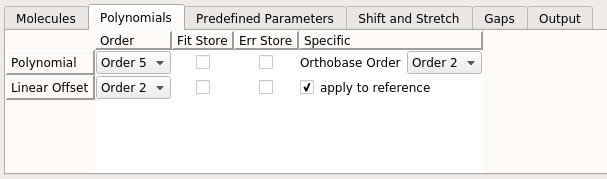
\includegraphics[width=\textwidth]{img/Analysis_Polynomials}
\caption{Analysis Windows Properties: Polynomial Page}\label{analysis_polynomial}
\end{figure}
\FloatBarrier

The values of the fitted coefficients account for the normalization
applied on both the spectrum and the reference. \textbf{Differential
  cross sections} can be generated by orthogonalisation of cross
sections w.r.t.\ an orthogonal base constructed out of the polynomial
components.  Generally, a base of order 2 is used. The
\textbf{OrthoBase} order column specifies the degree of this
orthogonal base.

To correct for instrumental and/or atmospheric straylight or residual
dark current signal, QDOAS can fit an offset parameter.  Normally,
offset is fit as a non-linear parameter, which can be configured in
the \textbf{Predefined Parameters} tab.  In some specific cases
(typically, in the near UV, around 300 nm), where the signal of the
spectrum is very low, it is better to fit offset as a linear
parameter, in order to avoid logarithm errors in when resolving the
DOAS equation (see section \ref{sec:offset-correction} for more
details).  When linear offset is enabled, a polynomial
$\mathrm{offset}(\lambda)$, normalized by the current spectrum is
included in to the DOAS fit:
\begin{equation}
\label{eq:linear_offset}
\mathrm{log}(I(\lambda))=\mathrm{log}(I_0(\lambda))-\sum{\sigma_ic_i}+\frac{\mathrm{offset}(\lambda)}{I(\lambda)}\,.
\end{equation}
The ``Order'' setting controls the order of the polynomial $\mathrm{offset}(\lambda)$.

Because the current spectrum appears in the denominator in equation
\eqref{eq:linear_offset}, QDOAS needs to solve a new linear system of
equations for every spectrum $I(\lambda)$, which can significantly
increase the processing time for a large analysis.  To work around
this, we can also apply the offset correction to the reference
spectrum, in which case the polynomial is normalized by the current
reference spectrum instead, and the fitting equation becomes
\begin{equation}
\label{eq:linear_offset_ref}
\mathrm{log}(I(\lambda))=\mathrm{log}(I_0(\lambda))-\sum{\sigma_ic_i}+\frac{\mathrm{offset}(\lambda)}{I_\mathrm{ref}(\lambda)}\,.
\end{equation}
This option can be enabled using the checkbox ``apply to reference''.

Note that a linear and a non-linear offset should not be fitted at the
same time in one spectral analysis window.

\subsection{The Predefined Parameters Pages}
This page proposes different parameters that can be fitted linearly or non linearly according to the fitting method:

\begin{itemize} \itemsep -6pt
\item scaling factor for the control spectrum (\textbf{Sol});
\item offset;
\item common residuals (\textbf{Com}).
\item undersampling (\textbf{Usamp1} and \textbf{Usamp2});
\item synthetic cross section to fit very small differences in the resolution between the spectrum and the reference (\textbf{Resol})
\end{itemize}

\begin{figure}[!h]
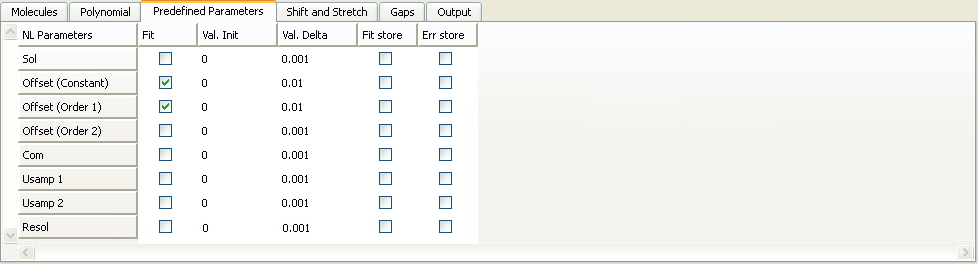
\includegraphics[width=\textwidth]{img/Analysis_Predefined.jpg}
\caption{Analysis Windows Properties: Predefined Parameters Page}\label{analysis_predefined}
\end{figure}
\FloatBarrier

A cross section file is always expected for \textbf{Com} parameter. A cross section file is expected for \textbf{Usamp1} and \textbf{Usamp2} parameters if the method \textbf{``File''} has been selected in the \textbf{Undersampling} page of \textbf{Projects properties}. To specify the name of the cross section file, right-click the \textbf{``Select~File''} option from the parameter line.

\textbf{Val init} and \textbf{Val delta} are respectively the initial value and convergence factor, two parameters used by the \gls{nlls} algorithm. In general, the default values should not be modified, except in case of convergence problems. \textbf{Fit store} and \textbf{Err store} columns are enabled only if the \textbf{Analysis button} is checked in the \textbf{Output} tab page of \textbf{Projects properties}.

\subsubsection{Offset}
An ideal spectrometer in an ideal atmosphere would measure the part of the sunlight that has been elastically scattered by air molecules and particles in the zenith direction. In a real experiment however a number of possible additional sources of signal may add up to the ideal Rayleigh/Mie contribution leading to ``offset'' the measured intensity by a certain amount. In addition to the Ring effect, which is to a first approximation a natural source of offset, instrumental sources of offset also need to be considered like stray light in the spectrometer and dark current of the detector. This is the purpose of the offset parameter which is better described in the \textbf{\nameref{cha:descr-algor}} chapter. The offset is normalized w.r.t. the intensity of the spectrum.

In some specific cases (typically, in the near UV, around 300 nm), the signal of the spectrum is very low and in order to avoid systematic logarithm errors when resolving the DOAS equation, the fit of a linearized offset is preferred (see the \textbf{Polynomial} page). Note that a linear offset and a non linear offset should not be fitted in the same spectral analysis window.

\subsubsection{Common residual}
When systematic structures appear in the residuals, it is sometimes useful to eliminate them using a synthetic cross section obtained by averaging some of such residuals (cfr the \textbf{``Residual''} field in the \textbf{Files} frame of this dialog box). In DOAS fitting, this cross section can be introduced either in the \textbf{Molecules} page with a user-defined symbol or in this page with the predefined symbol ``\textbf{Com}''. In intensity fitting, it is recommended to use the predefined symbol \textbf{Com} that is always fitted linearly whatever the analysis method.

\subsubsection{Undersampling} \label{sec:undersampling_params}
The undersampling is a well-known problem of GOME onboard the satellite ERS-2. It arises from the poor sampling ratio of the GOME instrument (2 to 3 pixels/\gls{fwhm} of the resolution of the spectrometer) which results in a lost of spectral information when interpolating earthshine spectra during the DOAS fitting process. The problem can be corrected using ad-hoc cross sections obtained by simulating the effect from a high-resolution solar reference. If the fit button of \textbf{Usamp 1} and/or \textbf{Usamp 2} items is checked, the options of the \textbf{Undersampling} page of \textbf{Project properties} (cfr page \pageref{sec:projects_undersampling_page}) are used to calculate undersampling cross sections.  In \textbf{From file} method, undersampling cross sections can be pre-calculated using the \textbf{QDOAS undersampling tool}.

\subsubsection{Resol synthetic cross section}
This cross section is built automatically by dividing the selected reference spectrum with itself but convolved with a gaussian with a FWHM of 0.05 nm.  It allows accounting for very small differences in the resolution of the reference spectrum and the spectrum to analyze.

\subsection{The Shift and Stretch Page} \label{sec:shift_stretch_page}
Shift and stretch parameters allow correcting for possible misalignment between the various spectral items involved in the data evaluation (i.e. measured and reference spectra as well as absorption cross sections). The equation below gives the wavelength transformation to apply when a shift and a stretch order 2 are fitted:

\begin{equation}
\Delta= a+b.(\lambda-\lambda_0)+c.(\lambda-\lambda_0)^2
\end{equation}

Less used, the scaling parameter consists in a wavelength dependent scaling factor to apply to a cross section. It can also be order 1 or order 2.

\begin{figure}[!h]
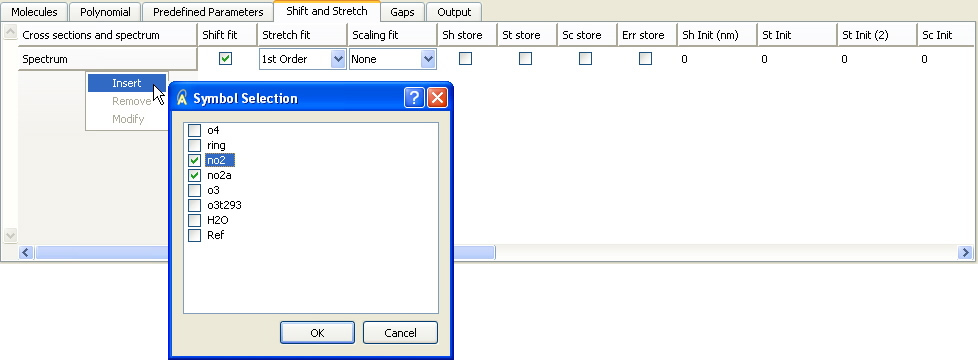
\includegraphics[width=\textwidth]{img/Analysis_Shift.jpg}
\caption{Analysis Windows Properties: Shift and Stretch Page}\label{analysis_shift}
\end{figure}
\FloatBarrier

To add an item to shift, stretch or scale, right-click the \textbf{Insert} option to open a dialog box with the list of available symbols (all cross sections defined in the \textbf{Molecules} page and completed with \textbf{Spectrum} and \textbf{Ref} symbols). It is possible to select only one or several symbols. In the latter case, the same shift and stretch parameters will be applied to all items of the selection (in the example above, the same shift and stretch will be applied on both \NO2 cross sections). After the validation of the selection, QDOAS automatically updates the list of available symbols so that a symbol can not be selected twice.

\textit{Note that a symbol can not be removed from the \textbf{Molecules} page as long as it is used in the \textbf{Shift and Stretch} page.}

\subsubsection{Output}
Buttons in the \textbf{Sh store}, \textbf{St store} and \textbf{Sc store} columns are enabled only if the \textbf{Analysis} button is checked in the \textbf{Output page} of \textbf{Projects properties}. They allow saving respectively the fitted values for the shift, the stretch and the scale. If buttons in the \textbf{Err store} column are checked, the standard deviations of the fitted parameters are also saved in the output file.

\subsubsection{Initial and delta values}
The shift, stretch and scale parameters are fitted non linearly by the Marquardt-Levenberg \gls{nlls} algorithm. This iterative method needs to start from an initial solution given by \textbf{Init} values of parameters to fit. The convergence parameters \textbf{Delta} are used by the algorithm to numerically calculate partial derivatives of the fitting function and to determine the direction of the steepest descent to approach the solution. There is one \textbf{Init} column and one \textbf{Delta} column for each parameter to fit (shift, stretch order 1, stretch order 2, scaling order 1 and scaling order 2).

\subsubsection{Convergence control}
In case of convergence problems or for safety reasons, the range of values allowed for the shift can be limited to a specified interval (\textbf{Sh Min} and \textbf{Sh Max}).

\subsection{The Gaps Page}\label{sec:analysis_gaps_page}
Gaps can be introduced in order to eliminate bad pixels from the fitting interval.  Note that using the ``Spikes removal'' feature (cfr page \pageref{sec:projects_analysis_spikes}) is a good alternative to automatically remove bad pixels.

\begin{figure}[!h]
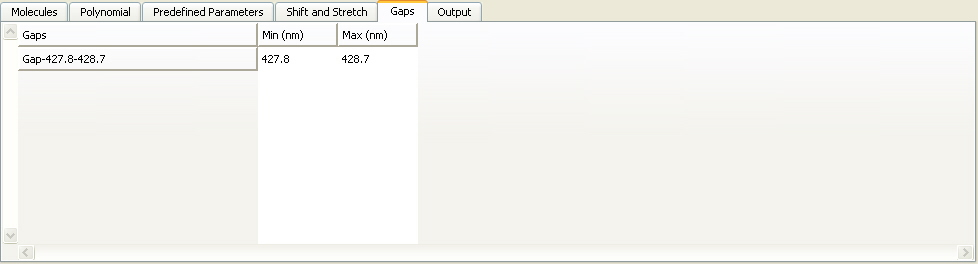
\includegraphics[width=\textwidth]{img/Analysis_Gaps.jpg}
\caption{Analysis Windows Properties: Gaps Page}\label{analysis_gaps}
\end{figure}
\FloatBarrier

\subsubsection{Insert a gap}
To insert a gap, right-click the \textbf{Insert} option and complete the \textbf{Min (nm)} and \textbf{Max (nm)} columns with the limits given in nanometers.  The first column is automatically updated after validation of the entry fields.

\subsubsection{Remove a gap}
To remove a gap, select it in the \textbf{Gaps} column and right-click the \textbf{Remove} option.

\subsection{The Output Pages}
For each cross section defined in the \textbf{Molecules} page, this page proposes to select the analysis results to save in the ASCII output file(s). Columns are enabled only if the \textbf{Analysis} button is checked in the \textbf{Output page} of \textbf{Projects properties}.

\begin{figure}[!h]
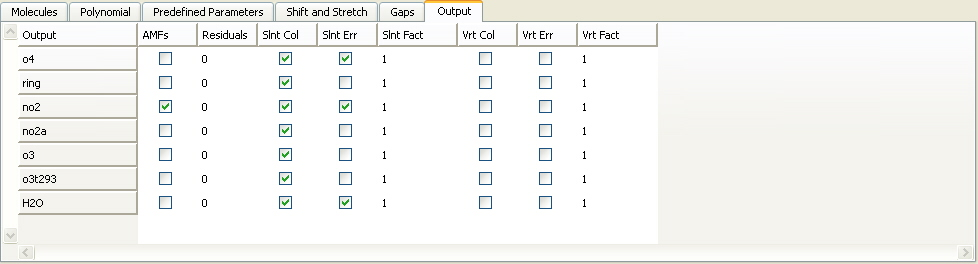
\includegraphics[width=\textwidth]{img/Analysis_Output.jpg}
\caption{Analysis Windows Properties: Output Page}\label{analysis_output}
\end{figure}
\FloatBarrier

QDOAS calculates and saves vertical columns if an \gls{amf} dependency has been selected in the \textbf{Molecules} page. The \textbf{Residuals} column gives the possibility to specify a value for the residual column amount of the selected species in the reference spectrum.

In the output file, slant columns and vertical columns (and their respective errors) can be divided by a scaling factor using \textbf{Slnt Fact} and \textbf{Vrt Fact} edit controls.

In the output file, the title of columns with the retrieval results always starts with the name of the analysis window. Slant columns are indicated by \textbf{SlCol}, standard deviations by \textbf{SlErr}, vertical columns by \textbf{VCol}, air mass factors \textbf{AMF}, etc\dots For example, if the application contains two analysis windows (no2 and o3), no2.slcol(o3) and o3.slcol(no2) refer to the column titles for respectively the slant columns of O3 in the no2 window and NO2 in the o3 fitting window.

Examples of output generated by QDOAS can be found in appendix \textbf{~\ref{cha:output}}.

\section{Configuration of the wavelength calibration procedure}\label{sec:conf-wavel-calibr}
The wavelength calibration facility developed in QDOAS is based on a
\gls{nlls} fitting procedure where the shift between the spectrum we
want to calibrate and a highly accurate solar reference spectrum is
determined on a series of short wavelength intervals.  The fitting
procedure uses the same algorithms used for the analysis of
spectra. The \textbf{Analysis Method} (optical density fitting or
intensity fitting) can be different from the one selected for the
analysis of spectra in the \textbf{Analysis page}.

The calibration procedure also allows the characterisation of the
instrumental slit function, through fitting of user-defined
\glspl{sfp}, either the \gls{fwhm} of an analytical line shape (see
the \textbf{\nameref{sec:analyt-line-shap}}, page
\pageref{sec:analyt-line-shap}) or two different stretch factors
applied on the grid of a user-defined function (option \textbf{File}).
If the slit function is not fitted during the wavelength calibration
procedure, the solar spectrum and the instrumental line shape to use
for convolutions are defined in the \textbf{Slit page}, page
\pageref{sec:projects_slit_page}.

The wavelength calibration can be applied to any kind of spectrum (the
reference spectra or spectra to analyze).

The wavelength calibration can be configured in the
\textbf{Calibration} page of the project properties.  We explain the
different settings below.

\begin{figure}[!h]
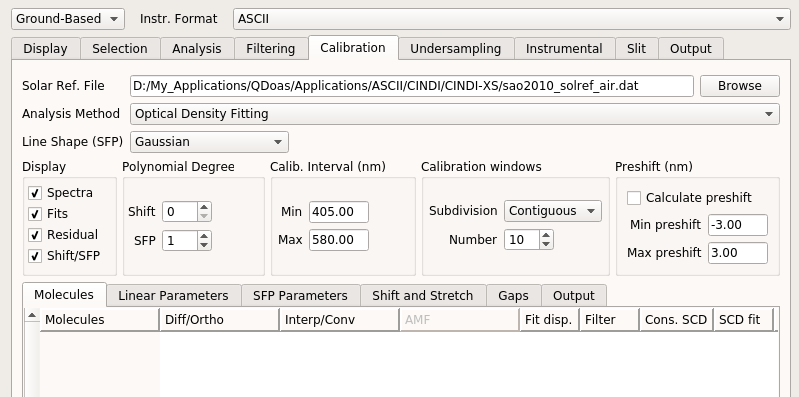
\includegraphics[width=\textwidth]{img/Project_Calibration.png}
\caption{Projects properties: Calibration page}\label{projects_properties_calibration}
\end{figure}
\FloatBarrier

\subsection{Solar Reference File and Line Shape}
There are two cases to consider:
\begin{enumerate}
\item The slit function (line shape) of the instrument is known and
  there is no need to characterise it once again (\textbf{Line Shape}
  ``Don't fit'').  Then the \textbf{Solar Ref. File} in this page is
  disabled; it should be given in the \textbf{Slit page}, together
  with the known instrumental line shape.
\item The slit function of the instrument needs to be characterized
  (selection of a \textbf{Line Shape}): the \textbf{Solar Ref. File}
  should contain a high-resolution solar spectrum.  Because the
  convolution algorithm in QDOAS uses the Fourier transform to speed
  up the \gls{nlls} fitting, a high-resolution solar spectrum sampled
  on a constant grid is expected.
\end{enumerate}

\subsection{Display}
When the calibration procedure is applied, a page named ``Kurucz''
appears in the plot area of the program except if the
\textbf{Calibration fits} button is unchecked in the \textbf{Display
  page}. This page includes four kinds of plots:

\begin{description}
\item[Spectra] the complete fit between the observed and the calculated spectra;
\item[Fits] fit of the Ring effect and/or atmospheric absorptions if any;
\item[Residual] the residual of the fit;
\item[Shift/SFP] the wavelength dependency of the shift and the slit function parameters over the whole detector.
\end{description}

\subsection{Polynomial Degree}
When the fitting procedure for each subwindow has finished, a
polynomial is used to approximate the shift values determined in each
subwindow.  This polynomial is then used to correct the initial
wavelength calibration.  Similarly, the wavelength dependent slit
function is determined by fitting a polynomial through the individual
SFP values. A different \textbf{polynomial degree} can be specified
for the shift and for the slit function.  The wavelength calibration
and the variation of the slit function thus determined are then used
e.g.\ to convolve high resolution cross sections before the analysis
of spectra and to build undersampling cross sections.

\subsection{Calibration Interval}
The wavelength interval used for the calibration must be specified in
the \textbf{Calib.\ Interval (nm)} frame. It should cover all the
spectral analysis windows defined under the \textbf{Analysis Windows}
node of the projects tree. This calibration interval is divided in a
number of \textbf{subwindows} and the shift and the \glspl{sfp} are
fitted using the \gls{nlls} approach within each of these subwindows.
The settings in the frame \textbf{Calibration windows} control the
definition of these subwindows.

\subsection{Calibration Windows}\label{sec:calibration-windows}
During the calibration procedure, the calibration interval is divided
into a number of smaller intervals.  The settings in the \textbf{Calibration
Windows} frame can be used to define these intervals.  The user can
set the number of intervals to be used, and set their limits using one
of the following options from the \textbf{Subdivision} drop-down menu:

\begin{description}
\item[Contiguous] With the default ``Contiguous'' option, the complete
  calibration interval is divided into non-overlapping subwindows of
  equal size.
\item[Sliding] The more general ``Sliding'' option allows the user to
  choose the width of the subwindows (``Size (nm)''), independently
  from the number of subwindows.  The calibration interval is now
  divided into a number of equally spaced subwindows, which can be
  made to overlap by choosing a larger size, or made disjoint by
  choosing a smaller size.  Usually, one wants to increase the size of
  the subwindows in order to improve the stability of the calibration
  fit in each subwindow.
\item[Custom] With the ``Custom'' option, the user can manually set
  the limits of the subintervals used in the calibration.  Clicking on
  the ``Define windows'' button opens a pop-up where the lower and
  upper wavelength limit can be configured for each subwindow.
\end{description}

\subsection{Fitting Parameters}
The wavelength calibration uses a similar property sheet as the
\nameref{analysis_properties} to configure the fitting procedure for
the calibration subwindows.  The configuration of these pages is
usually limited to the specification of the degree of the polynomial
uses in the DOAS equation (different from the polynomial used to build
the final grid from the individual values of the shift resulting from
the fit as described above), the slit function parameters to fit
according to the selection of the line shape and the shift between the
spectrum to calibrate and the solar spectrum. But the algorithm can
also take into account atmospheric absorption, Ring effect and offset
correction.

\subsubsection{The Molecules page}
The \textbf{Molecules} page allows introducing correcting absorbers that may optimise the accuracy of the wavelength calibration, e.g. the Ring effect (when calibrating a scattered-light spectrum) and \ozone~absorption can be taken into account in the fit.

\begin{figure}[!h]
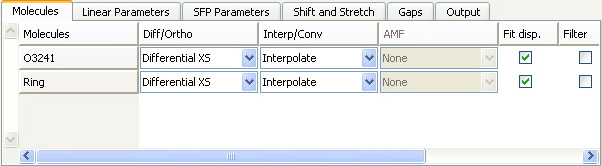
\includegraphics[width=.8\textwidth]{img/Calibration_Molecules.jpg}\hfill

\vspace{6pt}

\hfill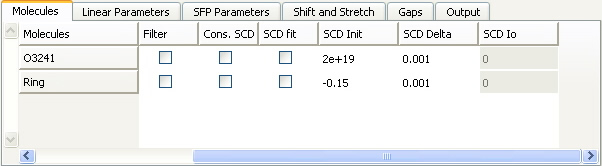
\includegraphics[width=.8\linewidth]{img/Calibration_Molecules2.jpg}
\caption{Calibration Properties: Molecules Page}\label{calibration_molecules}
\end{figure}

To generate differential cross sections (column \textbf{Diff/Orthog}), see page \pageref{differential_xs}.  The \textbf{Fit display} column is activated only if the \textbf{Calibration} button is checked in the \textbf{Display} page of \textbf{Projects properties} (see page \pageref{sec:projects_display_page}) and if the \textbf{Fits} button is checked in the \textbf{Display} frame of the \textbf{Calibration} page (see page \pageref{sec:projects_calibration_page}).  The selected cross section are usually pre-convolved with the resolution of the instrument and interpolated on the grid of the control (reference) spectrum.

In order to optimise the accuracy of the calibration (and given limitations inherent to the method), it is recommended to limit the number of parameters to fit and to constrain the slant column density of molecules.  This can be done in two passes:

\begin{itemize}
\item in the first pass, the column density is fitted (\textbf{SCD Fit} button is checked) over the whole calibration interval; a mean value of the concentration is then determined from the sub intervals where the fitting of the cross section has a sense (where the spectral information is largest);
\item in the second pass, the concentration is fixed at the mean value determined at the previous pass.
\end{itemize}

See previous section (\ref{sec:analysis_config_param}) for a complete description of the columns in this page.

\subsubsection{The Linear Parameters Page}
In this page, you define the polynomial used to approximate the
continuous component of the spectrum to calibrate.  To generate
differential cross sections using the orthogonalisation method, don't
forget to build an orthogonal base (see page
\pageref{differential_xs}).

\subsubsection{The Slit Function Parameters Page}
The fit of the \glspl{sfp} can be configured in this page.  There are
two predefined parameters -- SFP 1 and SFP 2 -- whose role depends on
the line shape chosen in the \textbf{Line Shape (SFP)} drop-down menu.
Note that if you do not want to fit the slit function during the wavelength
calibration procedure, select \textbf{Don't fit} in the Line Shape
menu and choose a solar reference spectrum and line shape in the
\textbf{Slit Page} of \textbf{Projects properties} (see page
\pageref{sec:projects_slit_page}) instead.

\begin{figure}[!h]
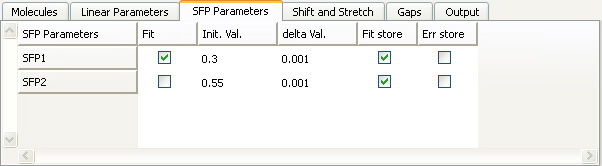
\includegraphics[width=\textwidth]{img/Calibration_Predefined2.jpg}
\caption{Calibration Properties: SFP Parameters Page (Parameterisation for an error function line shape)}\label{calibration_sfp}
\end{figure}

Table \ref{tab:sfp_meanings} provides an overview of the meaning of
SFP 1 and 2 for the different possible line shapes.  For analytical
line shapes, \textbf{SFP 1} is generally used for fitting the
\gls{fwhm} of the selected line shape.  The Voigt profile function is
the convolution of a Gaussian and a Lorentzian line shapes, where the
second parameter is the Lorentz/Gauss ratio.  Asymmetric line shapes
can be fitted by introducing an asymmetry factor in the Gaussian
formula.  For two-parameter line shapes, it is generally recommended
to fix one of the parameters to an estimated value in order to avoid
numerical instabilities.

\begin{table}\label{tab:sfp_meanings}
  \centering
  \setlength\tabcolsep{3.5pt} % default value: 6pt
  \begin{longtable}{lcc}
    \toprule
    & \textbf{SFP 1} & \textbf{SFP 2} \\
    \midrule
    \textbf{File}	& Stretch factor & Stretch factor \\
    & (negative wavelengths)	& (positive wavelengths)	\\
    \textbf{Gaussian}	& \gls{fwhm}	& Ignored \\
    \textbf{Error function}	& FWHM	& Boxcar width \\
    \textbf{2n-Lorentz}	& FWHM	& Ignored \\
    \textbf{Voigt profile}	& FWHM (Gaussian)	& Lorentz/Gauss ratio \\
    \textbf{Asymmetric Gaussian}	& FWHM (Gaussian)	& Asymmetry factor \\
    \bottomrule
  \end{longtable}
\caption{Meaning of the SFP parameters for different types of line
shape.}
\end{table}

\subsubsection{The Shift and Stretch Pages}
For the configuration of these pages, refer to the previous section (\ref{sec:shift_stretch_page}, page \pageref{sec:shift_stretch_page}).  In order to avoid the interpolation of the spectrum to calibrate, it is recommended to fit the shift of the high-resolution solar spectrum, represented by the symbol \textbf{Ref}.

\textit{In this case, all cross sections defined in the \textbf{Molecules} page have to be shifted with the solar spectrum.}

\begin{figure}[!h]
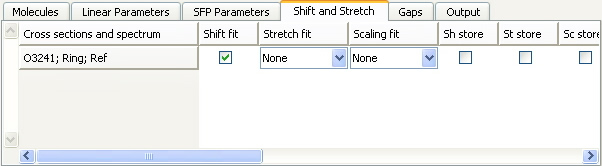
\includegraphics[width=\textwidth]{img/Calibration_Shift.jpg}
\caption{Calibration Properties: Shift Page (The \ozone~and Ring cross sections defined in the \textbf{Molecules} page are shifted with the solar spectrum.)}\label{calibration_shift}
\end{figure}

\subsubsection{Output}
Fitted slant column densities and non linear parameters are saved in the output file if the \textbf{``Calibration''} button is checked in \textbf{Output Page} of \textbf{Projects properties}.  This is particularly useful if a \textbf{Run Calibration} is performed on all spectra of the file.

\subsection{Calculation of the preshift} \label{sec:projects_calibration_preshift}
If the wavelength calibration of the reference spectrum is really too bad, the calibration procedure couldn't converge and return a wrong value of the shift that corresponds to a local minimum of the chi square.  In this case, it could be useful to approximate the value of the shift by calculating the
correlation between the reference spectrum and the solar spectrum convolved at the resolution of the instrument using the initial value(s) of the slit function parameter(s).  The value of the shift giving the best correlation will be introduced by the program as initial shift of the usual NLLS algorithm.
To calculate the preshift before the Kurucz procedure, check the \textbf{``Calculate preshift''} button in the \textbf{``Preshift (nm)''} frame and define the interval in nanometers wherein the shift values can vary for the correlation test.

%%% Local Variables:
%%% mode: latex
%%% TeX-master: "QDOAS_manual"
%%% TeX-PDF-mode: t
%%% End:

\chapter{The QDOAS Tools} \label{cha:tools}
QDOAS is delivered with four off-line modules :

\begin{itemize} \itemsep -6pt
\item \textbf{convolution} : a convolution/filtering tool;
\item \textbf{Ring} : a tool to create Ring effect cross sections;
\item \textbf{usamp} : a tool to create undersampling cross sections;
\item \textbf{doas\_cl} : a command line tool for batch processing.
\end{itemize}

The three first ones were already in WinDOAS. If they can still be called from
the QDOAS user interface, they are separate executables with their own user
interface, menu options and XML configuration files.

\section{The convolution/filtering tool (convolution)}\label{sec:conv-tool}

The \textbf{Convolution/Filtering} tool gives the possibility :

\begin{itemize}
\item to convolve spectra and cross sections;

\begin{itemize} \itemsep -6pt
\item user-defined slit functions and analytical line shapes are accepted;
\item convolution with $I_0$ correction is supported;
\end{itemize}

\item to shift the calibration grid before convolution;
\item to create an effective slit function taking into account the (finite) resolution
of the source spectrum (using a FT deconvolution method);
\item to apply a low-pass or a high-pass filter to the convolved cross section
before saving it.
\end{itemize}

\textbf{Convolution/Filtering} tool options are distributed in three pages :
\vskip 6pt
\begin{tabular}[h]{l p{8cm}}
\textbf{General} & general options (convolution type, input/output files...); \\ [6pt]
\textbf{Slit} & selection and parameterisation of the slit function; \\ [6pt]
\textbf{Filtering} & selection and parameterisation of the filter; \\ [6pt]
\end{tabular}

\begin{figure}[!h]
\subsection{The General Page}\hfill
\vspace{-.8\baselineskip}
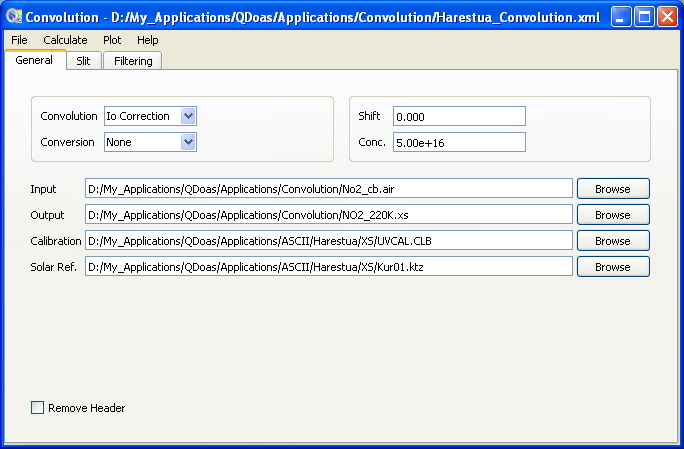
\includegraphics[width=1\textwidth]{img/Tools_Convolution_General.jpg}
\caption{Convolution/Filtering Tool} \label{tools_convolution_general}
\end{figure}
\FloatBarrier

\subsubsection{The Convolution Type}

QDOAS supports standard convolution and convolution with $I_0$ correction. The
convolution integral is calculated using the method of trapezes. If \textbf{None} is
selected, the cross section is just interpolated on the final grid.

\subsubsection{Conversion}

Before the convolution, it is possible to convert the original wavelength
calibration of the input cross section file from the air to the vacuum or inversely,
from the vacuum to the air.

\subsubsection{Requested Files Names}\hfill
\begin{tabular}[t]{l p{9.5 cm}}
\textbf{Input file} & the name of the high resolution cross section file to interpolate or convolve;   \\ [6pt]
\textbf{Output file} & the name of the resulting interpolated or convolved cross section file;  \\ [6pt]
\textbf{Calibration} & the final grid on which the original cross section (input file) must be interpolated or convolved;  \\ [6pt]
\textbf{Solar ref.} & the high-resolution solar spectrum requested only if the convolution with $I_0$ correction is selected;  \\ [6pt]
\end{tabular}

The format of input and output files is described in appendices \textbf{\ref{cha:input-files-format}} and \textbf{\ref{cha:output}}. The resulting cross section
file can be used as input for the retrieval. It is then better to give the
name of the output file in the format imposed by QDOAS : \textbf{cross section
files names must imperatively start with the symbol name as prefix
followed by the underscore character!}

\subsubsection{Shifting the Convolved cross section}

A shift in nm can be applied to the convolved cross section. In order to avoid
interpolation after convolution, this shift is applied on the calibration grid before
convolution.

\subsubsection{$I_0$ correction}

The fields \textbf{Solar Ref.} and \textbf{Conc} are respectively the name of the high resolution
solar spectrum file and the scaling column density of the concerned molecule.
Both are used for calculating the synthetic optical density in the formula of $I_0$
correction convolution. These fields are ignored if $I_0$ correction is not used.

\begin{figure}[!h]
\subsection{The Slit Function Page}\label{sec:slit-function-page}\hfill
\vspace{-.8\baselineskip}
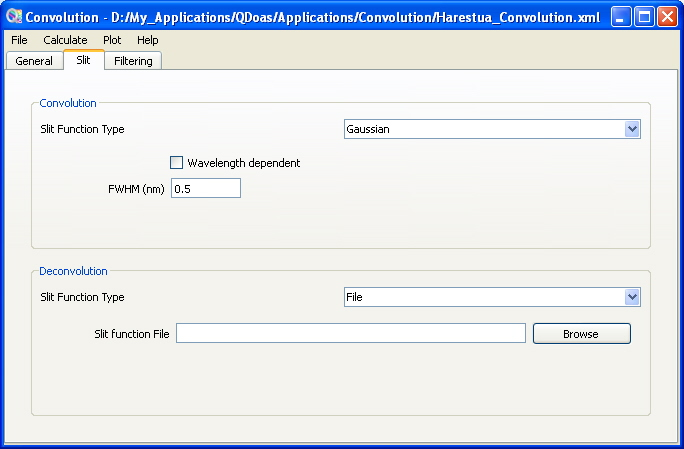
\includegraphics[width=1\textwidth]{img/Tools_Convolution_Slit.jpg}
\caption{Convolution/Filtering Tool: Slit Function page} \label{tools_convolution_slit}
\end{figure}
\FloatBarrier

This page is dedicated to the selection and the parameterisation of the convolution slit function.  Different analytical line shapes (Gaussian, Lorentzian, Voigt, error functions, asymmetric gaussian) are supported.  \textbf{QDOAS always requests the FWHM of the line shapes}.  The wavelength dependency of the slit function parameters characterized by the wavelength calibration procedure can be saved from the plot page in order to be accounted for the convolution.  Check the \textbf{Wavelength dependent} button to enter files instead of numbers.  Refer to the section \textbf{\nameref{sec:analyt-line-shap}} on page \pageref{sec:analyt-line-shap}, for further information on the supported analytical line shapes.

The use of arbitrary slit functions is possible with \textbf{File} option.  Look up table of slit functions defined at specific wavelengths is accepted.  If the \textbf{Wavelength dependent} button is checked, a three columns file is expected giving the variation of two different stretch factors to apply on the grid of the slit function.  Such a file can be obtained by merging in one file the SFP1 and SFP2 parameters resulting from the wavelength calibration procedure.

See file formats in \textbf{\nameref{cha:input-files-format} Annex}.


\subsubsection{Deconvolution}

A deconvolution slit function can also be defined.  In this case, the high resolution cross section is convolved using an effective slit function obtained from the FT of convolution and deconvolution slit functions.  This feature doesn’t work if a wavelength dependent slit function is selected.  By default, no deconvolution is applied.

\begin{figure}[!ht]
\subsection{The Filtering Page}\hfill
\vspace{-.8\baselineskip}
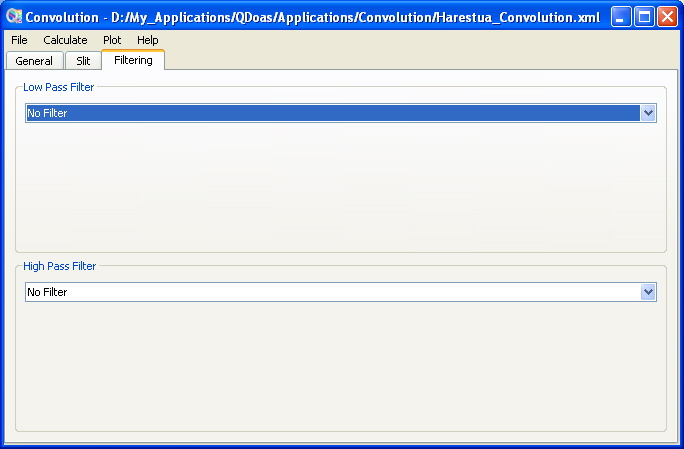
\includegraphics[width=1\textwidth]{img/Tools_Convolution_Filtering.jpg}
\caption{Convolution/Filtering Tool: Filtering page}
\label{tools_convolution_filtering}
\end{figure}
\FloatBarrier

After convolution, a low-pass and/or a high-pass filtering can be applied on the cross section.  By default, no filtering is applied.  The presentation of this page is the same as the \textbf{Filtering} one of \textbf{Projects properties}.  According to the selected filter type, the requested information can be different.

The original spectrum can be divided by the smoothed one or the smoothed spectrum can be subtracted from the original one.  The second feature is useful to create differential cross sections.

\subsubsection{The Convolution}

Once the parameters specified, the convolution is performed using the \textbf{Calculate $\rightarrow$ Run Convolution} option from the menu bar.   The original cross section and the convolved one (respectively in black and in red on the plot below) are displayed.  In order to avoid edge effects, the convolution has been performed on a larger interval but only the part of the convolved spectrum defined on the final grid is output.  If a filtering has been applied, another plot follows, with the original cross section and the resulting one after convolution and filtering.

\begin{figure}[!h]
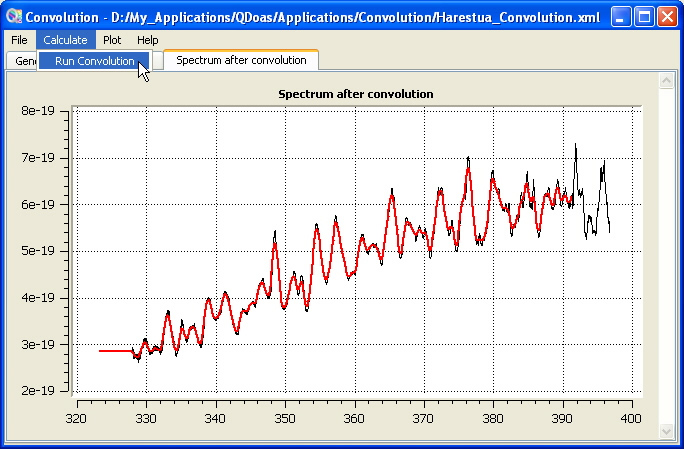
\includegraphics[width=1\textwidth]{img/Tools_Convolution.jpg}
\caption{Convolution with $I_0$ correction of a \NO2 cross section
  with a Gaussian (FWHM : 0.5 nm)
  \citep{vandaele1996}} \label{tools_convolution}
\end{figure}
\FloatBarrier

\section{The Ring tool (ring)}

The so-called Ring effect arises in the atmosphere due to inelastic scattering processes (mainly \gls{rrs} by molecular \oxygen{} and \N2). Roughly speaking, it manifests itself by a broadening of the solar and atmospheric spectral features present in measured spectra. This broadening typically reduces the depth of thin solar and atmospheric absorption features by several percents. Hence, it has a strong impact on spectroscopic measurements using the \gls{doas} method and retrieval algorithms must appropriately correct for it. This is especially true for minor absorbers like BrO or OClO, for which weak absorption features can be completely masked by Ring structures.

In DOAS, the Ring effect is usually accounted for as an absorber. The QDOAS Ring tool calculates Ring cross sections using a simple method described by \citet{Chance1997}.  See the \textbf{Description of Algorithms} chapter, page \pageref{sec:ring-effect} for further information on the Ring effect.

\begin{figure}[!h]
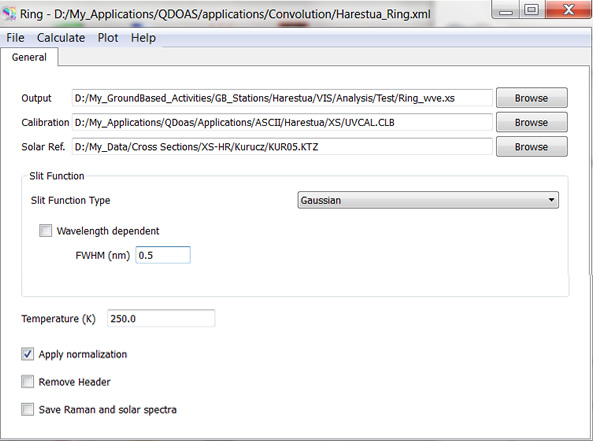
\includegraphics[width=1\textwidth]{img/Tools_Ring_General.jpg}
\caption{The Ring Tool}\label{tools_ring_general}
\end{figure}
\FloatBarrier

\subsubsection{Input}

QDOAS requires :

\begin{minipage}[t]{\textwidth}
\vspace{-1\baselineskip}
\begin{enumerate} \itemsep -6pt
\item the final grid on which the Ring cross section must be calculated;
\item a high-resolution solar spectrum;
\item the slit function to use for the convolution : user-defined slit functions and analytical line shapes (Gaussian, Lorentzian, Voigt and error functions) are accepted. The wavelength dependency of the line shape (Gaussian or error function) characterized by the wavelength calibration procedure can be saved from the plot page in order to be accounted for the convolution.
\end{enumerate}
\end{minipage}
\vskip 6pt
The effect of a change in temperature is small. Generally 250K is a good approximation for the atmospheric temperature at which most of the RRS is taking place.  The normalization of the Raman spectrum (see~\citep{Wagner2009}) is now optional

\subsubsection{Output}

As the calculated Ring cross section is accounted as an absorber, it is recommended to give the name of the output file in the format imposed by QDOAS : \textbf{cross section files names must imperatively start with the symbol name as prefix followed by the underscore characters!}

The Ring cross section is calculated as the ratio of the rotational
Raman spectrum by the solar spectrum (R/S).  The output file is an
ASCII file with two or four columns depending on whether the button ``Save
Raman and solar spectrum'' is checked or not: \vskip 3pt
\begin{minipage}[t]{\textwidth}
\vspace{-1\baselineskip}
\begin{itemize} \itemsep -6pt
\item the input wavelength calibration;
\item the calculated Ring cross section;
\item the interpolated Raman spectrum (optional);
\item the convolved solar spectrum (optional).
\end{itemize}
\end{minipage}
\vskip 6pt
To directly use the file as a cross section for the analysis without further convolution, only the first two columns should be saved (the program will display an error if the file contains unneeded columns).  If the \textbf{Convolve Ring} action is requested (see the \textbf{Molecules page} of \textbf{Analysis windows properties}), the program needs all four columns.  With ``Convolve Ring'', QDOAS uses the information on the slit function retrieved from the wavelength calibration procedure or from the slit function page to convolve the Raman and the solar spectra separately, and use the calculated ratio as a Ring cross section in the fit.

\begin{figure}[!h]
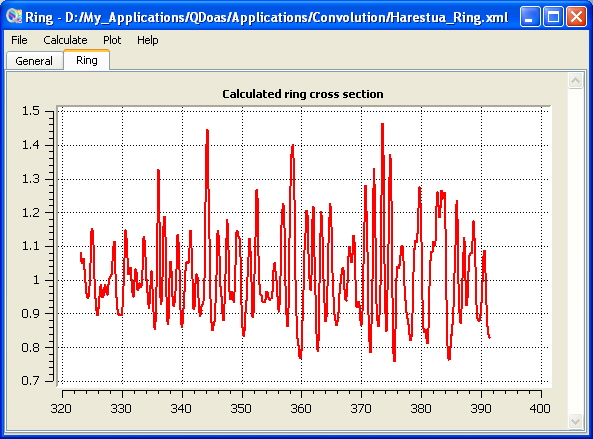
\includegraphics[width=1\textwidth]{img/Tools_Ring.jpg}
\caption{Ring cross section generated with the Ring Tool} \label{tools_ring}
\end{figure}
\FloatBarrier

\section{The undersampling tool (usamp)}  \label{sec:tool_undersampling}

The undersampling is a well-known problem of GOME onboard the satellite ERS-2. It arises from the poor sampling ratio of the GOME instrument (2 to 3 pixels/\gls{fwhm} of the resolution of the spectrometer) which results in a lost of spectral information when interpolating earthshine spectra during the DOAS fitting process. The problem can be corrected using ad-hoc cross sections obtained by simulating the effect from a high-resolution solar reference (see Chance K., 1998 \citep{Chance1998}).

The approach consists in building two spectra (an oversampled one and an undersampled one) from the high resolution solar spectrum and according to the selected analysis method, to calculate the ratio (DOAS fitting) or the difference (Intensity fitting) in order to simulate the interpolation error. Two undersampling cross sections are generated (the first one using the instrument grid and the second one using the instrument grid with a small shift applied).

See the \textbf{Description of Algorithms} chapter, page \pageref{sec:unders-corr}, for further information on the undersampling.

\begin{figure}[!h]
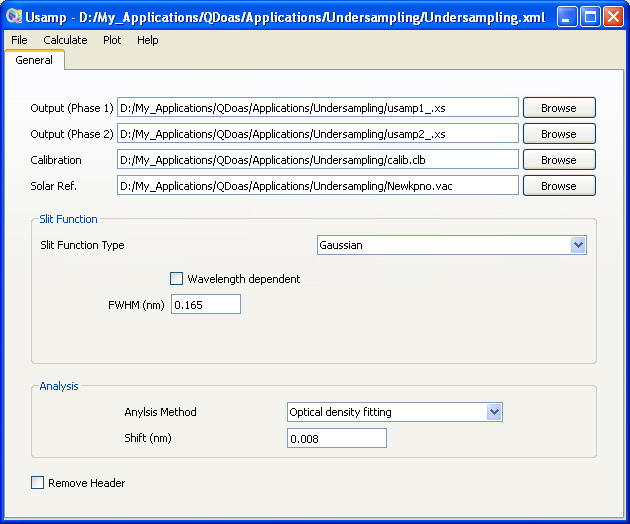
\includegraphics[width=1\textwidth]{img/Tools_Usamp_General.jpg}
\caption{The Undersampling Tool} \label{tools_usamp_general}
\end{figure}
\FloatBarrier

\subsubsection{Input}

QDOAS requires :

\begin{itemize}
\item the final grid on which the undersampling cross sections must be calculated;
\item a high-resolution solar spectrum;
\item the slit function to use for the convolution : user-defined slit functions and analytical line shapes (Gaussian, Lorentzian, Voigt and error functions) are accepted. The wavelength dependency of the line shape (Gaussian or error function) characterized by the wavelength calibration procedure can be saved from the plot page in order to be accounted for the convolution.
\item the shift to apply to oversampled and undersampled spectra in the calculation of undersampling;
\item the analysis method that determines the relation between oversampled and undersampled spectra;
\end{itemize}

\subsubsection{Output}

Two undersampling cross sections are generated by the procedure. It is recommended to give the name of the output files in the format imposed by QDOAS : \textbf{cross section files names must imperatively start with the symbol name as prefix followed by the underscore character~!}

\begin{figure}[!h]
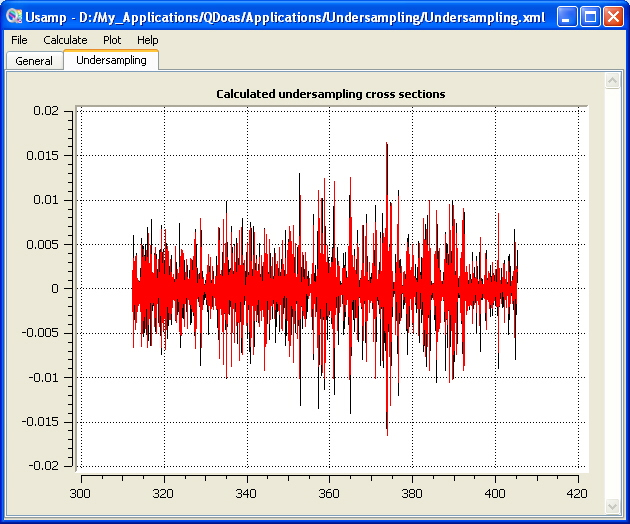
\includegraphics[width=1\textwidth]{img/Tools_Usamp_Plot.jpg}
\caption{Undersampling cross sections generated with the Undersampling Tool} \label{tools_usamp}
\end{figure}
\FloatBarrier

\section{The command line tool (doas\_cl)}

The QDOAS package includes a very powerful command line tool : doas\_cl.  It consists in a separate module to load from the command line with a xml configuration file (a QDOAS application or the configuration file built from the convolution/filtering, Ring or undersampling tool).

To see the syntax, just run doas\_cl without arguments :

\begin{Verbatim}[fontfamily=courier,fontsize=\relsize{-2}]
doas_cl -c <config file> [-a/-k <project name>] [-o <output>] [-f <file>] ...

    -c <config file>   : A QDoas, convolution, [Ring or usamp] config file.
                         The tool to invoke is determined from the type of
                         configuration file specified;

    -a <project name>  : for QDoas, run analysis on the specified project
    -k <project name>  : for QDoas, run calibration on the specified project

    -v                 : verbose on (default is off)

    -xml <path=value>  : advanced option to replace the values of some options
                         in the configuration file by new ones.
------------------------------------------------------------------------------
doas_cl is a tool of QDoas, a product jointly developed by BIRA-IASB and S[&]T
Last version : Qdoas version 2.1 - 20 December 2012
\end{Verbatim}

doas\_cl is useful to process large amount of files (for example
satellite data).  It takes spectrum files or directories containing
spectra as arguments.  An output file name different from the one
given in the \textbf{Output} page of \textbf{Projects properties} can
be specified.

When no -a or -k flag is present, QDOAS will perform the analysis on
all projects.

Example of doas\_cl command included in a bash file :

\begin{Verbatim}[fontfamily=courier,fontsize=\relsize{-2}]
/usr/local/bin/doas_cl -c "$HA_pathAnalysis/QDOAS_Harestua.xml" \
-a "Harestua" -o "$HA_pathAnalysisOutput/$year/automatic" -f "$HA_fileToProcess"
\end{Verbatim}

This command uses the QDOAS\_Harestua.xml file previously generated by
QDOAS.  It loads the project ``Harestua'' (important to specify if
several projects exist in the application).  The output file name is
generated automatically (see the \textbf{Output page} of
\textbf{Projects properties}).

\textbf{Important : always use slash as path separator for doas\_cl file arguments (input and output) even if you work under Windows.}

For the convolution tool, the switch -f applies only to one file but
the command can be called several times from a batch.  For the
\textbf{Ring tool}, the switch -f modifies the final calibration grid.
To change other parameters, it is better to write a piece of code to
modify the xml file.

\subsection{-xml switch}

In batch processing or in the frame of specific tests, it can be
useful to modify the original options of the configuration file
slightly.  For example, use another reference spectrum, slightly shift
a spectral window,...  The -xml command line switch allows the
modification of some configuration parameters.  It can only be used
when processing a single project, specified using the -a switch.

The xml configuration file is structured with blocks of options
delimited by start/end tags.

\begin{Verbatim}[fontfamily=courier,fontsize=\relsize{-2}]
<qdoas>
  <paths>
   ...
  </paths>
  <symbols>
   ...
  </symbols>
  <project name="MAXDOAS-VIS" disable="false">
    ...
    <analysis_window name="NO2" disable="false" kurucz="ref"
                     refsel="auto" min="425.000" max="490.000" >
      <display spectrum="true" poly="true" fits="true" residual="true"
               predef="false" ratio="true" />
      <files refone=""
             reftwo=""
             residual=""
             szacenter="0.000" szadelta="0.000" minlon="0.000" maxlon="0.000"
             minlat="0.000" maxlat="0.000" refns="0"
             cloudfmin="0.000" cloudfmax="0.000"
             maxdoasrefmode="sza"
             east="false" center="false" west="false" backscan="false" />
       ...
    </analysis_window>
    <raw_spectra>
      ...
    </raw_spectra>
  </project>
</qdoas>
\end{Verbatim}

Options related to a project are given within tags \texttt{<project
  ...>} and \texttt{</project>}.  A project includes one or more
\texttt{<analysis\_window ...>} and \texttt{</analysis\_window>}
blocks with analysis windows properties.

Given this structure, an option can be easily reached by building a
``path'' with the tags of the successive blocks it belongs to.  For
example, the option \textbf{Reference 1} of the \textbf{Analysis
  windows properties} can be reached by :

\begin{Verbatim}[fontfamily=courier,fontsize=\relsize{-2}]
/project/analysis_window/files/refone
\end{Verbatim}

To use a reference file other the one specified in the xml file, the
switch -xml in the doas\_cl command can be used as follows :

\begin{Verbatim}[fontfamily=courier,fontsize=\relsize{-2}]
-xml "/project/analysis_window/files/refone=<new file>"
\end{Verbatim}

It is recommended to quote the whole command.  If the name of the
analysis window is specified, the changes are applied only on this
window.  Otherwise, they will be applied to all analysis windows of
the project.

To modify the spectra range of the analysis window named NO2, two
successive \texttt{-xml} switches are used :

\begin{Verbatim}[fontfamily=courier,fontsize=\relsize{-2}]
doas_cl <...> -xml "/project/analysis_window/NO2/min=450"
              -xml "/project/analysis_window/NO2/max=490"
\end{Verbatim}

If the xml command is recognized, the following lines should be
displayed on the console :

\begin{Verbatim}[fontfamily=courier,fontsize=\relsize{-2}]
/project/analysis_window/NO2/min : 425.00 replaced by 450 (NO2)
/project/analysis_window/NO2/max : 490.00 replaced by 500 (NO2)
\end{Verbatim}

Not all options of the configuration file can be modified.  doas\_cl
will indicate if a field can not be changed.

%%% Local Variables:
%%% mode: latex
%%% TeX-master: "QDOAS_manual"
%%% TeX-PDF-mode: t
%%% End:

\appendix
\chapter{Input file formats}\label{cha:input-files-format}

\subsection{Spectra Files}\hfill
\begin{minipage}[t]{\textwidth}
\vspace{-0.6\baselineskip}
\begin{tabular}[h]{l p{8cm}}
\textbf{Used in} & Projects properties, Instrumental page \\ [6pt]
\textbf{File name} & no restriction; \\ [6pt]
\textbf{File extension} & \textbf{spe} by default, but it is not restrictive;  \\ [6pt]
\textbf{Format} & QDOAS supports a wide number of input formats, depending on the selected instrument in the project properties.  If QDOAS does not support the file format of the data you want to analyze, one option is to convert the data to the text-based QDOAS ASCII format, or the netCDF-based ``APEX'' format, which we describe below.\\  [6pt]
\end{tabular}
\end{minipage}

\subsubsection{ASCII Spectra File Format}
In order to work with data in the ASCII format, you should configure the detector size, i.e.\ the number of spectral channels, in the \textbf{Instrumental} tab of the project properties, and select one of the three available text-based input formats.  When using the \textbf{line format}, each line of the file should contain one spectrum record.   When using the \textbf{column format} or \textbf{column extended format}), each line contains one spectral value.

For the \textbf{line} and the \textbf{column} formats, QDOAS will try to read the values selected using the checkboxes the \textbf{Instrumental page} of \textbf{Projects properties}.  These values should be provided strictly in the following order:
\begin{itemize} \itemsep -6pt
\item Solar Zenith Angle
\item Azimuth Viewing Angle
\item Elevation Viewing Angle
\item Date in the DD/MM/YYYY (day, month, year) format
\item Fractional time
\end{itemize}

Example of records in an ASCII file in \underline{\textbf{line format}} with solar zenith angle, date and fractional time options checked:

\begin{Verbatim}[fontfamily=courier,fontsize=\relsize{-2}]
   78.417543 29/02/2000 8.181111 5504.343400...  25379.428769
   77.426307 29/02/2000 8.356389 7568.723923...  25736.597692
   76.444749 29/02/2000 8.536944 8371.684631...  27477.536662
                                 <----- spectra values ----->
\end{Verbatim}

Below, an example of records in \underline{\textbf{column format}} with lambda, solar zenith angle, elevation viewing angle and decimal time options checked:

\begin{Verbatim}[fontfamily=courier,fontsize=\relsize{-2}]
   59.7336                     <- SZA
   1                           <- elevation viewing angle
   16.0452752135897            <- decimal time
     415.53904  4.1053669e+005
     415.57920  5.1616777e+005
     ...                           Wavelength and spectra values
     456.10521  5.0256531e+005
     456.14444  4.9851523e+005
   58.6879                     <- record number 2
   5
   15.953346969803
     415.53904  5.1705925e+005
     415.57920  6.5113944e+005
     ...
     456.10521  6.4016200e+005
     456.14444  6.3482669e+005
   60.4205                    <- record number 3
   10
   16.1055305555417
     415.53904  5.2111045e+005
     415.57920  6.5623468e+005
     ...
     456.10521  6.4077000e+005
     456.14444  6.3549114e+005
\end{Verbatim}
An ascii file in column format may also contain multiple columns with spectra.  Using the same input configuration as the previous example, the following file is also valid:

\begin{Verbatim}[fontfamily=courier,fontsize=\relsize{-2}]
             0  59.7336           58.6879           60.4205                              <- SZA
             0  1                 5                 10                                   <- elevation viewing angles
             0  16.0452752135897  15.953346969803   16.1055305555417                     <- decimal times
     415.53904  4.1053669e+005    5.1705925e+005    5.2111045e+005
     415.57920  5.1616777e+005    6.5113944e+005    6.5623468e+005
     ...
     456.10521  5.0256531e+005    6.4016200e+005    6.4077000e+005
     456.14444  4.9851523e+005    6.3482669e+005    6.3549114e+005
\end{Verbatim}
When using the column format, QDOAS assumes the following conventions:
\begin{itemize}
\item The wavelength calibration is always provided in the first column.
\item Each line of the file must contain no more than 4096 characters.
\item The file can contain multiple data blocks, but all data blocks should have the same number of columns.  If the wavelength calibration is read from the input file, it should be repeated in the first column of each block.
\end{itemize}

QDOAS also supports a \textbf{Column extended format}, more flexible than the two previous ones.  Spectra (optionally preceeded by wavelengths) are provided as column vectors and records can be described by $<$ KEYNAME $> = <$ KEYVALUE $>$ lines
where KEYNAMES are the names of pre-defined fields from the following list, according to the type of measurement:

\begin{Verbatim}[fontfamily=courier,fontsize=\relsize{-2}]
  Name
  Date (DD/MM/YYYY)
  UTC time (hh:mm:ss)
  Number of scans
  Exposure Time
  Solar Zenith Angle
  Solar Azimuth Angle
  Longitude
  Latitude
  Altitude
  Viewing elevation angle
  Viewing azimuth angle
  Viewing zenith angle
  Total Measurement Time (sec)
  Total Acquisition Time (sec)
  Start Date (dd/mm/yyyy)
  End Date (dd/mm/yyyy)
  UTC Start Time (hh:mm:ss)
  UTC End Time (hh:mm:ss)
  Measurement Type
\end{Verbatim}

A file in \textbf{Column extended format} can begin with comment lines starting with a hash (\texttt{\#}) character. Exposure time is also called integration time.  Total acquisition time should be the exact time needed by the device
to take the acquisition of non rejected scans.  Total measurement time should include the overheads requested by the measurement (for example, reading time, time to calculate the integration time, to move a pointing system...).
Spectra exported in ASCII by QDOAS are in \textbf{Column extended format}.

Example of a file in \textbf{Column extended format}:

\begin{Verbatim}[fontfamily=courier,fontsize=\relsize{-2}]
# Station = Cabauw (51.97 N,4.93 E)
# Institute = My institute
# PI name = my name and or my email
# Instrument = name of the instrument (or the channel)
# Size of the detector = 2048 (the size of the detector as indication)
# Total number of records = 548
Date(DD/MM/YYYY) = 24/09/2016
UTC Time (hh:mm:ss) = 10:38:05
UTC Start Time (hh:mm:ss) = 10:37:34
UTC End Time (hh:mm:ss) = 10:38:35
Viewing Elevation Angle (deg) = 5.0
Viewing Azimuth Angle (deg) = 135.0
Measurement Type (OFFAXIS/DIRECT SUN/ALMUCANTAR/ZENITH) = OFFAXIS
Total Measurement Time (sec) = 61
Total Acquisition Time (sec) = 1.848
Exposure Time(sec) = 0.033
Solar Zenith Angle (deg) = 53.9151
Solar Azimuth Angle (deg) = 163 (North=0, East=90)
      423.039410      1168041.606061
      423.159620      1195344.636364
      423.279810      1189587.060607
      423.399990      1160496.151516
      ...
      539.695430      1187768.878789
      539.804180      1219738.575758
      539.912910      1084799.181819
Date(DD/MM/YYYY) = 24/09/2016
UTC Time (hh:mm:ss) = 10:39:15
UTC Start Time (hh:mm:ss) = 10:38:45
UTC End Time (hh:mm:ss) = 10:39:45
Viewing Elevation Angle (deg) = 15.0
Viewing Azimuth Angle (deg) = 135.0
Measurement Type (OFFAXIS/DIRECT SUN/ALMUCANTAR/ZENITH) = OFFAXIS
Total Measurement Time (sec) = 60
Total Acquisition Time (sec) = 1.815
Exposure Time(sec) = 0.033
Solar Zenith Angle (deg) = 53.8636
Solar Azimuth Angle (deg) = 163.4 (North=0, East=90)
      423.039410      1309890.090910
      423.159620      1342920.393940
      423.279810      1336768.878789
      423.399990      1304920.393940
      ...
      539.695430      1076102.212122
      539.804180      1092465.848486
      539.912910      1023405.242425
Date(DD/MM/YYYY) = 24/09/2016
UTC Time (hh:mm:ss) = 10:40:30
UTC Start Time (hh:mm:ss) = 10:40:00
UTC End Time (hh:mm:ss) = 10:41:00
Viewing Elevation Angle (deg) = 89.9
Viewing Azimuth Angle (deg) = 135.0
Measurement Type (OFFAXIS/DIRECT SUN/ALMUCANTAR/ZENITH) = ZENITH
Total Measurement Time (sec) = 60
Total Acquisition Time (sec) = 9.353
Exposure Time(sec) = 0.199
Solar Zenith Angle (deg) = 53.8099
Solar Azimuth Angle (deg) = 163.8 (North=0, East=90)
      423.039410       252900.597990
      423.159620       258121.703518
      423.279810       256473.462312
      423.399990       250413.160805
      ...
      539.477900       142795.070352
      539.586670       142307.633166
      539.695430       140528.738694
      539.804180       144910.648242
      539.912910       125800.095478
\end{Verbatim}

\subsubsection{APEX File Format}\label{sec:apex-file-format}
The APEX format uses netCDF files containing radiance data, a wavelength calibration, and the essential variables needed to describe the viewing geometry for satellite observations.  Users who want to analyze satellite observations for instruments whose original format is not supported by QDOAS, or synthetic test data, can convert the required data to this format.

In the APEX format, observed radiances are stored as a three-dimensional array \texttt{row\_dim} x \texttt{col\_dim} x \texttt{spectral\_dim}.  The dimension \texttt{row\_dim} orders successive measurements (this dimension is called ``scanline'' in many satellite instrument formats).  For imager-type instruments, the \texttt{col\_dim} dimension describes the across-track position of a measurement, or the ground pixel.  If \texttt{col\_dim} is larger than one, QDOAS will perform a separate calibration for each ``column''\footnote{Note that for many imagers, such sa TROPOMI or OMI, this dimension is also referred to as the detector ``row'', not to be confused with the \texttt{row\_dim} of the APEX format.}.  For non imager-type instruments, where a single calibration should be used for all observations \texttt{col\_dim} should be equal to one.

The following cdl template describes the expected format of APEX netCDF input files, for an imager instrument with 10 detector pixels and a spectral dimension of 1280.
\begin{Verbatim}[fontfamily=courier,fontsize=\relsize{-2}]
netcdf apex_spectra {
dimensions:
	col_dim = 10 ; // cross-track dimension.  should be > 1 only for imagers
	row_dim = 100 ; // along-track dimension, order successive measurements
	spectral_dim = 1280 ;
variables:
	double radiance(row_dim, col_dim, spectral_dim) ;
	double radiance_wavelength(spectral_dim) ;
	double solar_zenith_angle(row_dim, col_dim) ;
	double viewing_zenith_angle(row_dim, col_dim) ;
	double relative_azimuth_angle(row_dim, col_dim) ;
	double latitude(row_dim, col_dim) ;
	double longitude(row_dim, col_dim) ;
}
\end{Verbatim}
In order to analyze spectra in the APEX format, the user must provide a reference spectrum in a specific netCDF format as well.  The following cdl template describes the expected format of the APEX reference spectrum.
\begin{Verbatim}[fontfamily=courier,fontsize=\relsize{-2}]
netcdf apex_reference {
dimensions:
	col_dim = 10 ;
	spectral_dim = 1280 ;
variables:
	double reference_radiance(col_dim, spectral_dim) ;
	double reference_wavelength(spectral_dim) ;
}
\end{Verbatim}
Note that the \texttt{col\_dim} of the reference spectrum and the spectra you want to fit, must be the same.

\subsection{Calibration}\hfill
\begin{minipage}[t]{\textwidth}
\vspace{-0.6\baselineskip}
\begin{tabular}[h]{l p{8cm}}
\textbf{Used in} & Projects properties \\
                 & Tools \\ [6pt]
\textbf{File name} & 	no restriction;  \\ [6pt]
\textbf{File extension} & \textbf{clb} by default, but it is not restrictive;  \\ [6pt]
\textbf{Format ASCII} & \textbf{Column 1}: the wavelength calibration; \\ [6pt]
\textbf{Example} & ANYTHING.CLB
\end{tabular}
\end{minipage}

\subsection{Cross sections}\label{sec:cross-sections}\hfill
\begin{minipage}[t]{\textwidth}
\vspace{-0.6\baselineskip}
\begin{tabular}[h]{l p{8cm}}
\textbf{Used in} & Analysis windows properties \\
                 & Tools \\ [6pt]
\textbf{File name} & In order to add a cross section to the list of fitted molecules for an analysis window in QDOAS (see section \ref{sec:molecules-page}), the cross section file name must start by the name of the corresponding symbol, followed by an underscore.  There is no restriction on the cross section file names in the other QDOAS tools. \\ [6pt]
\textbf{File extension} & \textbf{xs} by default, but it is not restrictive; \\ [6pt]
\textbf{Example} & BrO\_W228.XS
\end{tabular}
\end{minipage}
\subsubsection{ASCII format}
Cross sections can be provided as ASCII text files with columns of floating point numbers, separated by spaces.  The first column always contains the wavelength calibration for the cross section, and subsequent columns contain the cross section values.  When using a pre-convolved cross section for an imager instrument, the file should contain a column of convolved cross section values for every row of the detector.  When using a high-resolution cross section with online convolution, or when using a pre-convolved cross setion for an instrument with a single detector row, only one column of cross section values is expected.  ASCII cross section files may contain comments: text lines starting with characters \texttt{\#}, \texttt{*} or \texttt{;} are ignored.

\subsubsection{NetCDF format}
Cross sections can also be read from a NetCDF file.  Because NetCDF files store data in a binary format, this will typically be more efficient in terms of disk space as well as processing time.  The time savings can be significant when working with pre-convolved cross sections for imagers with a largen number of rows, such as TROPOMI or TEMPO.

A NetCDF cross section file for QDOAS should contain 2 variables: a vector \texttt{wavelength} containing the cross section wavelength calibration, and a 2-dimensional matrix \texttt{cross\_section} containing the cross section values.  In the case of a pre-convolved cross section for imager instruments, the number of columns in the cross section matrix (NetCDF dimension \texttt{dim\_y}) should be equal to the number of detector rows.  The following cdl template describes the expected fomat of the NetCDF file.  In this example, the size of dimension \texttt{dim\_y} is 60, which corresponds to the number of detector rows of the OMI UV/VIS bands.

\begin{Verbatim}[fontfamily=courier,fontsize=\relsize{-2}]
netcdf symbolname_cross_section {
dimensions:
	n_wavelength = 500 ;
	dim_y = 60 ; // 1 if single detector instrument or not pre-convolved

group: QDOAS_CROSS_SECTION_FILE {
  variables:
  	double cross_section(dim_y, n_wavelength) ;
  	double wavelength(n_wavelength) ;
  }
}
\end{Verbatim}
For simplicity, this example does not use NetCDF compression.  To further reduce disk space usage, you may enable zlib compression for the \texttt{cross\_section} variable by setting attributes such as
\texttt{\_DeflateLevel}, \texttt{\_Storage}, \texttt{\_ChunkSizes} and \texttt{\_Shuffle}.

\subsection{Solar Spectrum}\hfill
\begin{minipage}[t]{\textwidth}
\vspace{-0.6\baselineskip}
\begin{tabular}[h]{l p{8cm}}
\textbf{Used in} & Projects properties \\
                 & Tools \\ [6pt]
\textbf{File name} & no restriction; \\ [6pt]
\textbf{File extension} & \textbf{ktz} by default, but it is not restrictive; \\ [6pt]
\textbf{Example} & KUR\_01.KTZ
\end{tabular}
\end{minipage}

As is the case for cross sections, the user can either provide a solar spectrum at high resolution and let QDOAS compute the convolution with the instrument response function before analysis, or the user can provide pre-convolved solar spectra.  When using pre-convolved spectra for imager instruments, a convolved solar spectrum is required for every row of the detector.  The ASCII format for solar spectra is identical to that described in the previous section \nameref{sec:cross-sections}.  QDOAS can also read a solar spectrum from a NetCDF file, which should conform to the structure described in the following cdl file:

\begin{Verbatim}[fontfamily=courier,fontsize=\relsize{-2}]
netcdf solar_spectrum {
dimensions:
	n_wavelength = 500 ;
	dim_y = 60 ; // for preconvolved solar spectra of a 60-row imager, e.g. OMI
variables:
	float qdoas_matrix(dim_y, n_wavelength) ;
	float wavelength(n_wavelength) ;
}
\end{Verbatim}

Again, the file size can be reduced by enabling NetCDF compression for the variable \texttt{qdoas\_matrix}.

\subsection{Reference spectrum}\hfill
\begin{minipage}[t]{\textwidth}
\vspace{-0.6\baselineskip}
\begin{tabular}[h]{l p{8cm}}
\textbf{Used in} & Analysis windows properties \\ [6pt]
\textbf{File name} & no restriction;  \\ [6pt]
\textbf{File extension} & \textbf{ref} by default, but it is not restrictive; \\ [6pt]
\textbf{Format ASCII} & \textbf{Column 1}: the wavelength calibration \\
                      & \textbf{Column 2}: the reference spectrum \\ [6pt]
\textbf{Example} & 80302191.REF
\end{tabular}
\end{minipage}

\subsection{Instrumental function}\hfill
\begin{minipage}[t]{\textwidth}
\vspace{-0.6\baselineskip}
\begin{tabular}[h]{l p{8cm}}
\textbf{Used in} & Project properties \\ [6pt]
\textbf{File name} & no restriction; \\ [6pt]
\textbf{File extension} & \textbf{ins} by default, but it is not restrictive; \\ [6pt]
\textbf{Format ASCII} & \textbf{Column 1}: the wavelength calibration \\
                      & \textbf{Column 2}: the transmission function (spectra will be divided by this curve before the wavelength calibration procedure).\\ [6pt]
\textbf{Example} & Transmission.ins
\end{tabular}
\end{minipage}


\subsection{Dark current and Offset (ex.: MFC)}
Used in \textbf{Projects properties}.  Dark currents and offset are corrections specific to the selected instrument, so they have to be provided in the original format.

\subsection{AMF}\hfill
\begin{minipage}[t]{\textwidth}
\vspace{-0.6\baselineskip}
\begin{tabular}[h]{l p{8cm}}
\textbf{Used in} & Analysis windows properties \\ [6pt]
\textbf{File name} & The name of \gls{amf} file associated to cross sections implied in the definition of analysis windows must start by the user defined relevant symbol followed by an underscore; \\ [6pt]
\textbf{File extension} & AMF\_SZA  for \gls{sza} dependent AMF; \\
                        & AMF\_CLI  for climatology dependent AMF; \\
                        & AMF\_WVE  for wavelength dependent AMF; \\ [6pt]
\textbf{AMF\_SZA Format} & \textbf{Column 1}: SZA \\
                        & \textbf{Column 2}: AMF \\ [6pt]

\textbf{AMF\_CLI Format} &\begin{minipage}[t]{\textwidth}
                          \vspace{-0.6\baselineskip}
                          \begin{tabular}[h]{|p{2cm}|p{2cm}|}
                          \hline
                          0	& (JD-1)/365 \\
                          \hline
                          SZA & AMF \\
                          \hline
                          \end{tabular}
                          \end{minipage}
                          \vskip 12pt
                          Climatology dependent AMF have to be provided in a matrix whose first column is SZA grid and first line, day number grid. \\ [6pt]

\textbf{AMF\_WVE Format} &\begin{minipage}[t]{\textwidth}
                          \vspace{-0.6\baselineskip}
                          \begin{tabular}[h]{|p{2cm}|p{2cm}|}
                          \hline
                          0	& $\lambda$ \\
                          \hline
                          SZA & AMF \\
                          \hline
                          \end{tabular}
                          \end{minipage}
                          \vskip 12pt
                          Interpolation is made in a 2-dimension matrix (first column is SZA grid and first line, some wavelengths). \\ [6pt]

\textbf{Example} &  BrO\_W228.AMF\_SZA
\end{tabular}
\end{minipage}

\subsection{Slit functions}\hfill
\begin{minipage}[t]{\textwidth}
\vspace{-0.6\baselineskip}
\begin{tabular}[h]{l p{9cm}}
\textbf{Used in} & Analysis windows properties	\\ [6pt]
\textbf{File name} & no restriction; \\ [6pt]
\textbf{File extension} & \textbf{slf}  by default, but it is not restrictive; \\ [6pt]
\textbf{Format ASCII} & \textbf{Column 1}: the wavelength calibration \\
                      & \textbf{Column 2}: the line shape \\ [6pt]
                      & The slit function has to be provided with a wavelength calibration around 0 nm.  \\ [6pt]
                      & For wavelength dependent slit function types, the second column is the parameter dependent on the wavelength. \\ [6pt]
                      &	Since QDOAS version 2.00, lookup tables of wavelength dependent slit functions can be provided.  In this case, the number of columns depends on the available slit functions.  Wavelengths are specified in the first line of the file.  \\ [6pt]
\textbf{Example} &
\begin{minipage}[t]{\textwidth}
\vspace{-0.6\baselineskip}
\begin{Verbatim}[fontfamily=courier,fontsize=\relsize{-2}]
  0                         340                      380
 -1.00  2.9802322387695299e-008  7.8886090522101049e-031
 -0.98  5.9192925419630987e-008  1.2276631396533808e-029
 -0.96  1.1594950525907111e-007  1.8074887363782194e-028
 -0.94  2.2399967890119956e-007  2.5176165401687836e-027
 ...
 -0.04  9.7265494741228542e-001  8.9502507092797223e-001
 -0.02  9.9309249543703593e-001  9.7265494741228542e-001
  0.00  1.0000000000000000e+000  1.0000000000000000e+000
  0.02  9.9309249543703593e-001  9.7265494741228542e-001
  0.04  9.7265494741228542e-001  8.9502507092797223e-001
...
  0.94  2.2399967890119956e-007  2.5176165401687836e-027
  0.96  1.1594950525907111e-007  1.8074887363782194e-028
  0.98  5.9192925419630987e-008  1.2276631396533808e-029
  1.00  2.9802322387695299e-008  7.8886090522101049e-031
\end{Verbatim}
\end{minipage}   \\
&   \\ [6pt]
& \textbf{Specific case}: For wavelength dependent arbitrary slit function files (including lookup tables of slit functions), the variation of the two stretch factors to apply on the grid of the line shape is given in a three-columns file. \\ [6pt]
\end{tabular}
\end{minipage}

%%% Local Variables:
%%% mode: latex
%%% TeX-master: "QDOAS_manual"
%%% TeX-PDF-mode: t
%%% End:

\chapter{Output}\label{cha:output}

Information related to the measurements (e.g. date and time, viewing angles, geolocation data,~\ldots) can be selected in the \textbf{Display} and the \textbf{Output pages} of \textbf{Projects properties}. The selected instrument or file format determines the list of fields available in this page. For example, information on cloud fraction and cloud top pressure is available only for satellite instruments. A non-exhaustive list of fields available for ground-based and satellite measurements is given in figure \ref{fig:output_fields}.

The measurement type is available for CCD EEV and MFC BIRA-IASB MAXDOAS formats.  The convention is :

\begin{itemize} \itemsep -6pt
\item 1 for off axis
\item 3 for zenith sky
\item 4 for dark currents
\item 8 for offsets
\end{itemize}

\begin{figure}
\centering
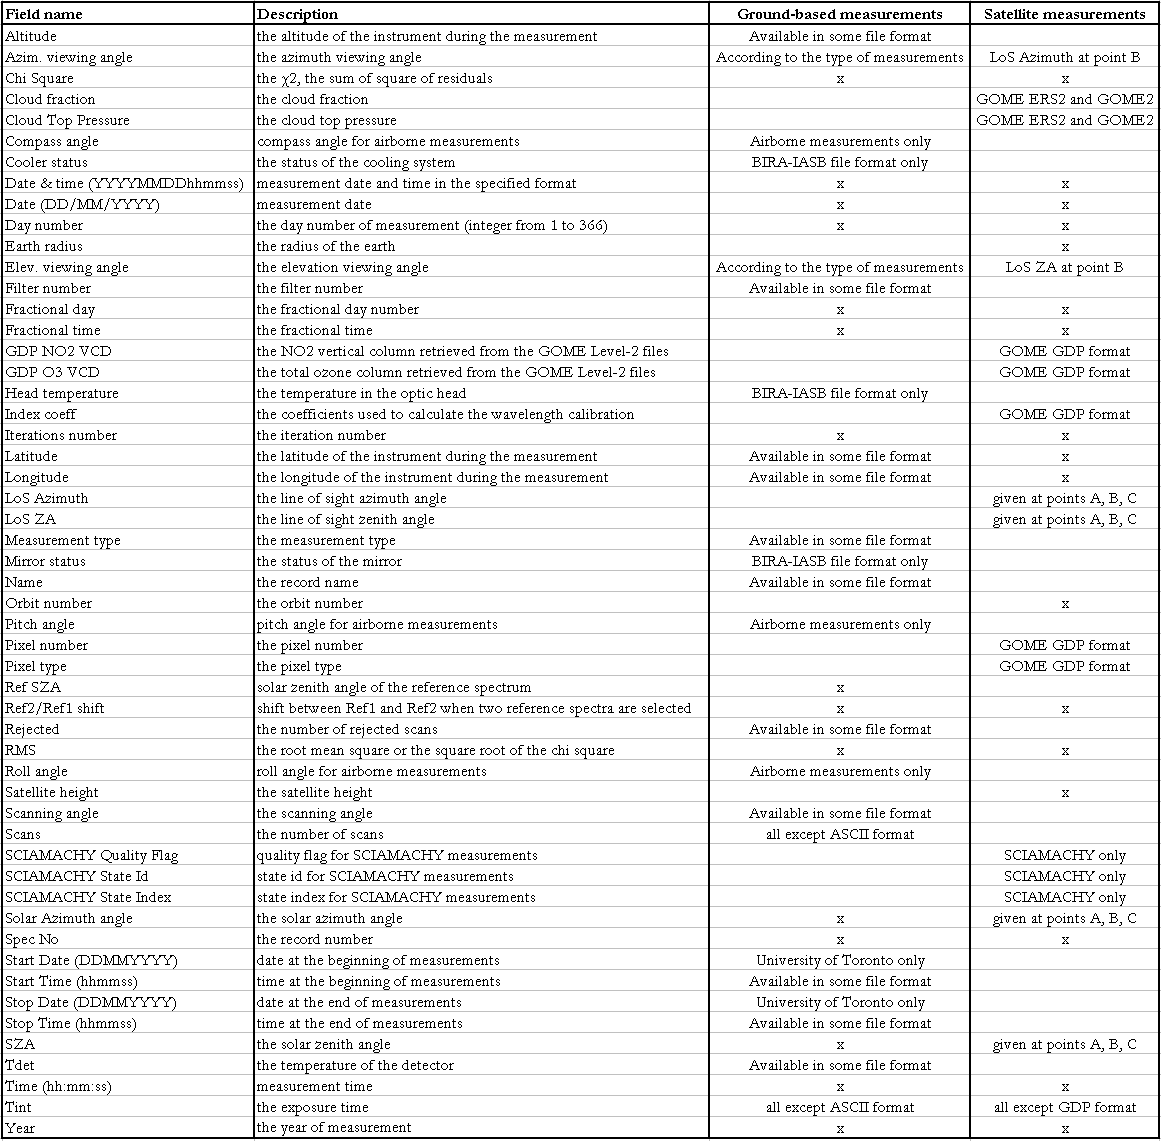
\includegraphics[width=\textwidth]{img/Output_Field.png}
\caption{A list of some of the output fields available in QDOAS.}\label{fig:output_fields}
\end{figure}

\begin{figure}
\centering
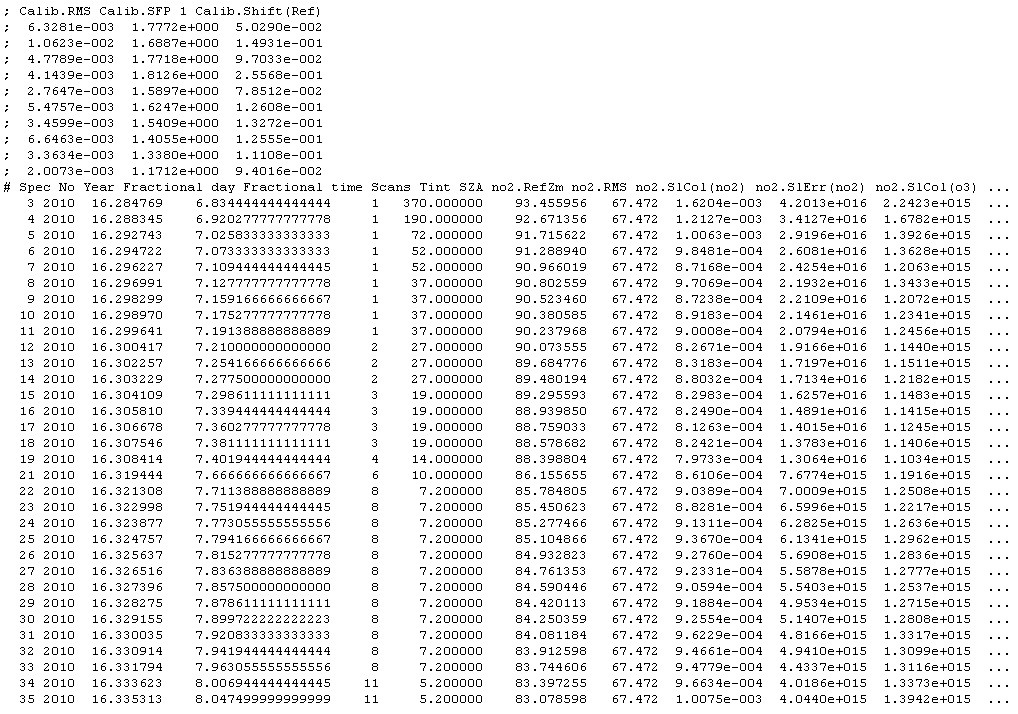
\includegraphics[width=\textwidth]{img/Output_Sample3.png}
\caption{Example of ASCII output generated by QDOAS.}\label{fig:ascii_output}
\end{figure}

In ASCII output files, columns are separated using tab characters and it is normal that they are not aligned with the column titles when the file is loaded in a simple text editor.  Figure \ref{fig:ascii_output} provides an example.  For this application, the \textbf{calibration button} is checked and results of the calibration procedure precede the analysis results. The \gls{rms}, the shift between the reference spectrum and the solar spectrum and the calculated value of the \gls{fwhm} of the fitted line shape (Gaussian in this application) for each of the sub-windows of the wavelength calibration interval are saved (see the \textbf{Calibration page} of \textbf{Projects properties} for further details).

The output in figure \ref{fig:ascii_output} contains the following fields:

\begin{enumerate} \itemsep -6pt
\item The record number (Spec No)
\item The year of measurements
\item The fractional calendar day
\item The fractional time
\item The number of scans
\item The exposure time (Tint)
\item The solar zenith angle (SZA)
\item The shift calculated between the spectrum and the reference in the no2 analysis window (no2.RefZm)
\item The \gls{rms} of the fit in the ? ``no2" analysis window (no2.RMS)
\item The slant column of \NO2 calculated in the  "no2" analysis window (no2.SlCol(no2))
\item The error on the slant column of NO2  (no2.SlErr(no2))
\item The slant column of \ozone calculated in the  ``no2" analysis window  (no2.SlCol(O3))
\item ...
\end{enumerate}

\begin{tabular}[h]{l p{3cm}}
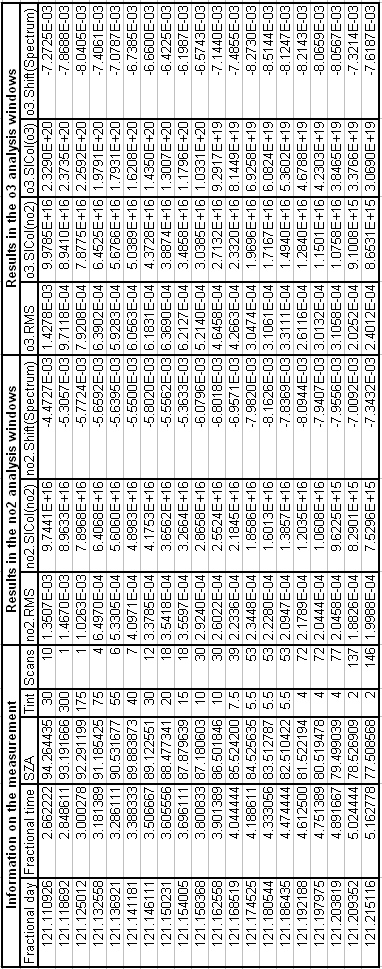
\includegraphics[height=24cm]{img/Output_Sample1.png} &
    \rotatebox{90}{\parbox{24cm}{\textbf{Example of output generated by QDOAS and loaded using Excel.} \\ In this example, only the fractional date and time, the solar zenith angle (SZA), the exposure time (Tint) and the number of scans have been selected in the \textbf{Output page} of \textbf{Projects properties}.  The application contains two analysis windows (no2 and o3).  In this example, the NO2 column has been retrieved from both no2 and o3 windows. The column title starts with the name of the analysis window.  Slant columns are indicated by \textbf{SlCol}; errors on slant columns by \textbf{SlErr} (not present in this example).}}
\end{tabular}

\begin{tabular}[h]{l p{3cm}}
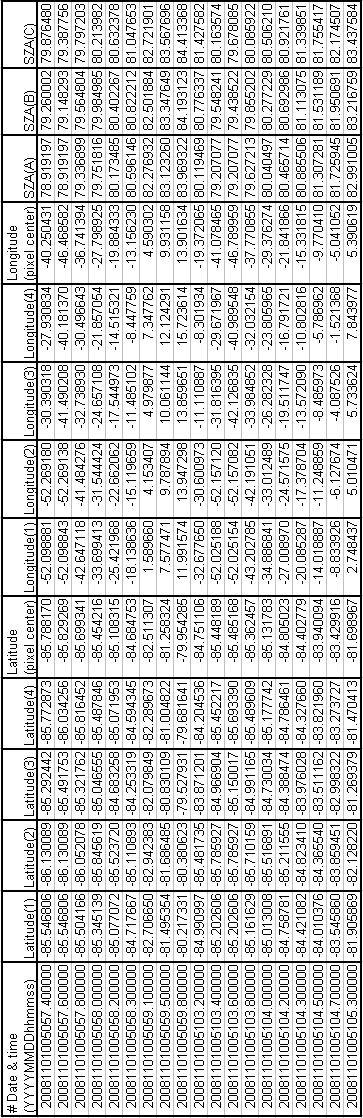
\includegraphics[height=24cm]{img/Output_Sample2.png} &
    \rotatebox{90}{\parbox{24cm}{\textbf{Example of output file generated by QDOAS and loaded using Excel.} \\ This example has been generated from a satellite application (GOME-2).  Results of the fit are not shown here.  For satellite measurements, the accuracy of the measurement time is important.  The format YYYYMMDDhhmmss (year, month, day, hour, minute, second accolated; milliseconds in the fractional part) is usually preferred to the fractional date and time.  Geolocation coordinates are given at the four corners and at the centre of the pixel. Angles such as the solar zenith angles are given at the beginning, the middle and the end of the measurement.}}
\end{tabular}


%%% Local Variables:
%%% mode: latex
%%% TeX-master: "QDOAS_manual"
%%% TeX-PDF-mode: t
%%% End:

\chapter{Troubleshooting}\label{cha:troubleshooting}

This section describes some problems that could be met with the user interface or some error messages displayed by QDOAS.  Most of error messages come from a wrong configuration (calibration or analysis settings).   If you can not solve a problem or if you have detected a bug, it's important to contact authors.  The log file produced by QDOAS in the application directory is an important source of information for us.  A small application with a detailed description of the trouble and the sequence of manipulations leading to it can help us to solve the problem quickly.

\section{Known user interface problems}

\subsection{Refreshing Problem In The Projects Properties}\hfill
\begin{figure}[!h]
\begin{minipage}[t]{\textwidth}
\vspace{-1.8\baselineskip}
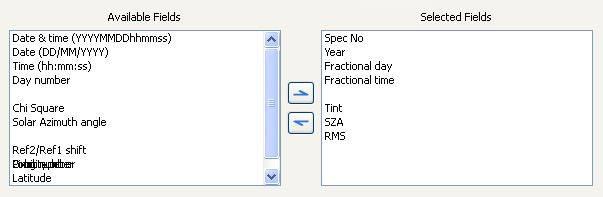
\includegraphics[width=\textwidth]{img/TroubleShooting_Output.jpg}
\end{minipage}
\end{figure}
\FloatBarrier

In the \textbf{Display} and the \textbf{Output pages} of \textbf{Projects properties}, the list of available fields that can be selected for display or output depend on the file format.  There is a problem with the refreshing of the list (missing fields or overwritten fields) after the selection of a new instrument or file format.  The list is correctly refreshed after quitting the \textbf{Projects properties} dialog box on \textbf{OK} and load it again.

All selected fields in the output page will be in the \textbf{output file} but some selected fields in the \textbf{Display page} could still have no effect on the display in the \textbf{Data page}.

\section{Analysis problems}\label{sec:analysis-problems}

\subsection{Calibration problems}\label{sec:calibration-problems}

Most problems usually come from the original wavelength calibration of the reference spectrum.  QDOAS corrects small shifts but the \gls{nlls} algorithm may not converge if the initial values are too far away from the solution (convergence to a local minimum of the chi-square).   Before using QDOAS, it is recommended to determine the preliminary wavelength calibration with a mercury lamp or to pre-convolve a solar spectrum at the resolution of your instrument, plot it with your spectrum and fit a polynomial through some pixels/nm couples set from the most representative Fraunhofer lines.  In the example below, even if the calcium lines match between the reference spectrum and the solar spectrum convolved at the resolution of the instrument, we can see that the wavelength calibration is completely wrong below 380 nm.  The differences are too large for QDOAS and it is better to correct that manually before running the calibration procedure.

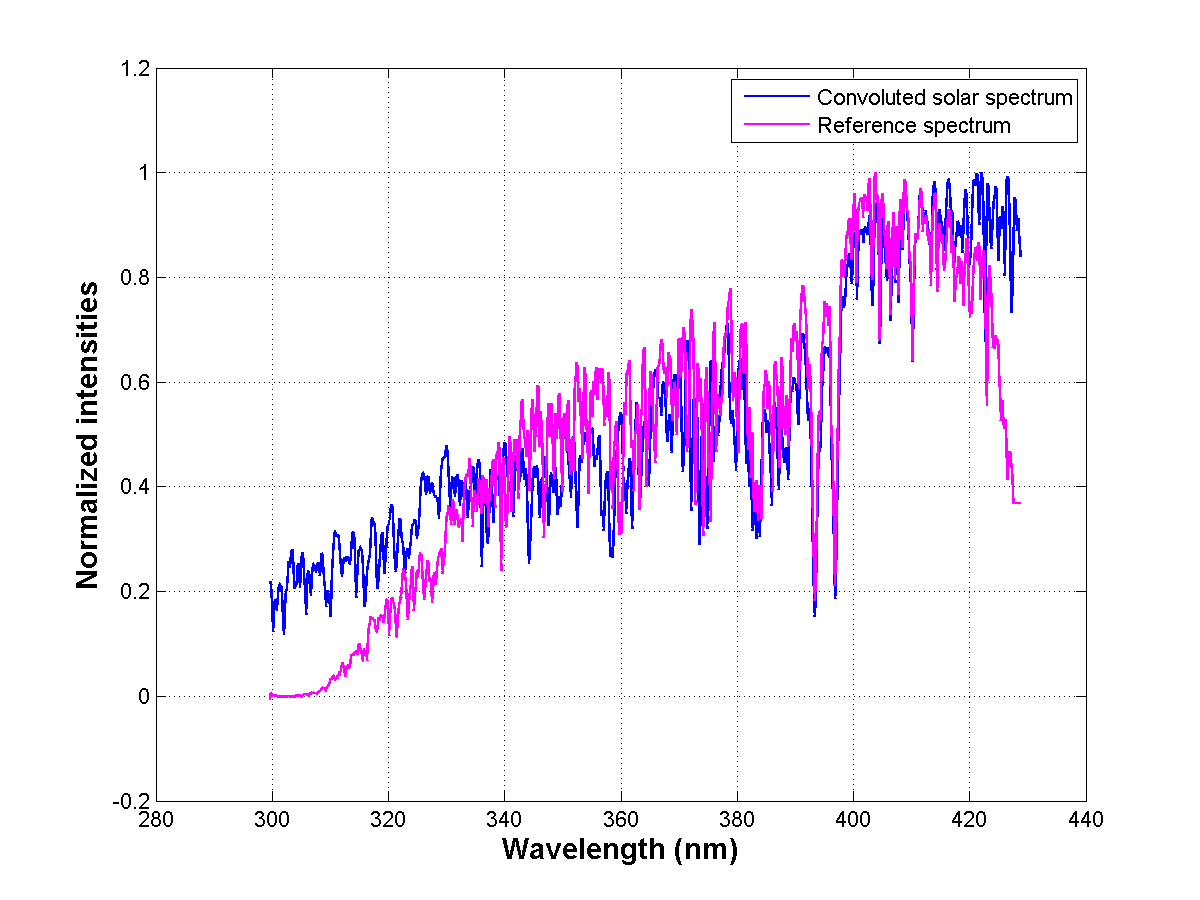
\includegraphics[width=\textwidth]{img/TroubleShooting_Calibration.jpg}

\subsection{Analysis error messages}

\textbf{Log error :}

\hspace{1cm}\parbox{11.5cm}{This message occurs mainly when the signal of the spectrum is too poor.  Usually, the message can be ignored if the cause can be identified : poor light conditions during twilight... If this error is systematic, the fit of a linear offset can be preferred to a non linear one (see page \pageref{eq:linear_offset}) or the fitting interval can be adjusted to another region where the signal is higher.}

\textbf{Sqrt argument error :} \\
\textbf{Curfit error :} \\
\textbf{Ill-conditioned matrix :}
\vskip 6pt
\hspace{1cm}\parbox{11.5cm}{These two messages are usually related to a problem with the configuration.

Check that all cross sections are defined in the fitting interval.  This can be done by right-clicking the \textbf{``View cross sections''} option from the analysis windows items.

Eventually, reduce the number of fitting parameters to the minimum (just the polynomial) and proceed step by step in order to identify the problem.

If the problem occurs during the calibration procedure, report to the section \textbf{``Calibration problems''} above.}

\textbf{Allocation error during the Kurucz procedure :}

\hspace{1cm}\parbox{11.5cm}{The degree of the polynomial fitting the continuous part of spectrum has not been defined in the \textbf{``Linear parameters page''} (see \textbf{Calibration page} of \textbf{Projects Properties}, page \pageref{sec:projects_calibration_page}).}

\textbf{spline interpolation requests increasing abscissae (...) :}

\hspace{1cm}\parbox{11.5cm}{The problem can come from a bad input file (preliminary wavelength calibration in the \textbf{``Instrumental page''} of \textbf{Projects properties}, cross section, reference spectrum) or the wavelength calibration procedure doesn't succeed to correct the preliminary wavelength calibration (report to the section \textbf{``Calibration problems''} above).}

\textbf{Number of degree of freedom $<=$ 0... :}

\hspace{1cm}\parbox{11.5cm}{Too many parameters are fitted w.r.t. the size of the fitting interval or the settings of the filter are not suitable.  Reduce the number of parameters to fit, increase the fitting interval or adjust the size of the filter.  Check also the calibration settings (Calibration page of Projects Properties).}

\textbf{Cross section file is empty or not large enough :}

\hspace{1cm}\parbox{11.5cm}{Check that all cross sections are defined in the fitting interval.  This can be done by right-clicking the \textbf{``View cross sections''} option from the analysis windows items.   Do not also forget the cross sections and the solar spectrum defined in the Calibration page of Projects Properties.}

%%% Local Variables: 
%%% mode: latex
%%% TeX-master: "QDOAS_manual"
%%% TeX-PDF-mode: t
%%% End: 



\printglossaries

%\include{QDOAS_annex}
%\bibliographystyle{plainnat} % harvard % apalike

\nocite{numericalrecipe_2007,numericalrecipes_1992,Wagner2009a,Wagner2010}
\nocite{Kuruczsolar,Hermans1999,Burrows1999,Bogumil2003}

\bibliographystyle{apalike}
\bibliography{QDOAS_biblio}
\end{document}

%%% Local Variables:
%%% mode: latex
%%% TeX-master: t
%%% TeX-PDF-mode: t
%%% End:
